% LTeX: language=fr
\documentclass[11pt]{report}
\usepackage{lib/utc-report-template}
\usepackage{lib/glossaire}
\usepackage{subcaption}
\usepackage{placeins}
\usepackage{biblatex}
\usepackage{amssymb}
\usepackage{graphicx} % Pour inclure les images
\usepackage{wrapfig}  % Pour le placement à côté du texte
\usepackage{tabularx}
\usepackage{hyperref}
\DeclareUnicodeCharacter{202F}{\,}
\addbibresource{references.bib}

% Meta informations
\author{Macéo NARBONNET}

\setcounter{secnumdepth}{2}


\begin{document}
    % Import des macros si besoin
    \include{lib/macro}

    %Creation de la page de garde
    \frontpage

    \pagenumbering{arabic}

    \chapter*{Remerciements}

  J'aimerais commencer par remercier l'ensemble du labo BMBI de m'avoir accueilli pendant six mois dans de très bonnes conditions. Un grand merci aux chercheurs et doctorants de l'équipe E-Biomed pour les réunions autour de délicieux gâteaux et cafés. Je tiens à remercier les étudiants avec lesquels j'ai pu travailler, notamment les TX qui m'ont aidé dans les tests du système MoCapIA et la comparaison avec le système Vicon. Merci donc à \textbf{Juliette LAFONT}, \textbf{Dorian BIOT}, mais aussi leurs amis (aussi appelé \textit{cobaye}) pour nous avoir permis d'élargir la base de donnée. Je tiens également à remercier \textbf{Lucas LAGEL} pour nous avoir consacré du temps et ainsi permis l'utilisation du robot UR3 (Universal Robot 3). Merci à \textbf{Théophile COCQUEREZ}, \textbf{Julie PROCOPE-MAMERT} et \textbf{Guillaume TOFFOLI} pour l'entraide entre nos différents projets ainsi qu'à \textbf{P. TRIGANO} pour ses conseils lors de la rédaction du rapport, en espérant les avoir correctement appliqués. Enfin, j'aimerais remercier \textbf{Khalil Ben MANSOUR} pour son encadrement, son soutien et ses conseils tout au long de ce stage.



    % Sommaire
    \setcounter{tocdepth}{1}
    \tableofcontents
    \setlength{\parskip}{1em}    % Définit l'espace entre deux paragraphes
    \setlength{\parindent}{2em}  % Définit la taille de l'alinéa

    % Les parties du rapport
    \chapter{Résumé Technique}

\vspace{\fill}

   Ce stage s'est déroulé au sein de l'équipe BioMovE, une division du laboratoire BMBI (BioMécanique et BioIngénieurie) de l'UTC. L'objectif principal du stage est de développer et d'améliorer un logiciel de capture de mouvement \textbf{sans marqueurs} (aussi appelé \textbf{markerless motion capture}). Basé sur l'intelligence artificielle et la vision par ordinateur, ce logiciel nommé \textbf{MoCapIA} permet de capturer le mouvement humain en 3D à partir de vidéos prises par plusieurs caméras synchronisées. Contrairement aux systèmes traditionnels de capture de mouvement qui utilisent des marqueurs physiques attachés au corps, MoCapIA offre une solution plus flexible et moins coûteuse pour l'analyse du mouvement.
   
   Ce stage s'inscrit dans la continuité de quatre autres stages réalisés les quatre derniers semestres (A23, P24, A24, P25 respectivement intitulés MoCapIA-1, MoCapIA-2, MoCapIA-3 et MoCapIA-4). Durant ces précédents stages, les principales fonctionnalités de base du logiciel ont été développées. Le principe de base de \textbf{calibration}, de \textbf{détection} et de \textbf{reconstruction 3D} du mouvement ont été implémentés. Pour MoCapIA-5, l'objectif est de calculer la précision, d'améliorer la robustesse et la précision du logiciel en intégrant de nouvelles fonctionnalités et en optimisant celles déjà développées. Une interface avait aussi été déjà développée en amont et son amélioration/optimisation reste un objectif secondaire de ce stage (plutôt dédié à la deuxième stagiaire présente avec moi durant le semestre). Il utilise PyQt5 orienté objet et les nouvelles fonctionnalités y seront intégrés.
   
   Toujours en python orienté objet, la partie "mathématique" du logiciel utilise plusieurs bibliothèques open-source telles que OpenCV pour le traitement d'images, NumPy pour les calculs numériques, ainsi que plusieurs modèles d'intelligence artificielle pré-entraînés pour la détection des points clés du corps humain dans les images 2D (TensorFlow, PyTorch, RTMPose, YOLO, ...). Ce sont ces fonctionnalités que le stage vise à améliorer notamment pour atteindre une précision suffisante pour une analyse biomécanique. En ce sens, de nouveaux packages et fonctionnalités autour d'OpenSim (un logiciel open-source de simulation musculo-squelettique) et de la bio-cinématique seront intégrés.

    
  \vspace{\fill}
\vfill
    \chapter{Introduction}

    L'innovation en matière de vision par ordinateur et d'intelligence artificielle ne cesse de progresser, souvent à des vitesses impressionnantes. Cette tendance ouvre de nouvelles perspectives passionnantes dans divers domaines, notamment celui de la capture de mouvement. C'est dans ce contexte que s'inscrit ce stage TN09 que j'ai eu l'opportunité de réaliser au sein de l'équipe BioMov-E du laboratoire BMBI (BioMécanique et BioIngénieurie) de l'UTC. Hier encore, les solutions en matières de motion capture reposaient principalement sur des systèmes utilisant des marqueurs physiques attachés au corps des sujets. Mais avec l'émergence de nouvelles technologies de vision par ordinateur et surtout d'intelligence artificielle, les solutions \textbf{markerless} deviennent de plus en plus crédible. Développer et mesurer la fiabilité de telles solutions est l'objectif principal de ce stage.

\section{Présentation du labo BMBI}
    \begin{figure}[h]
        \centering
        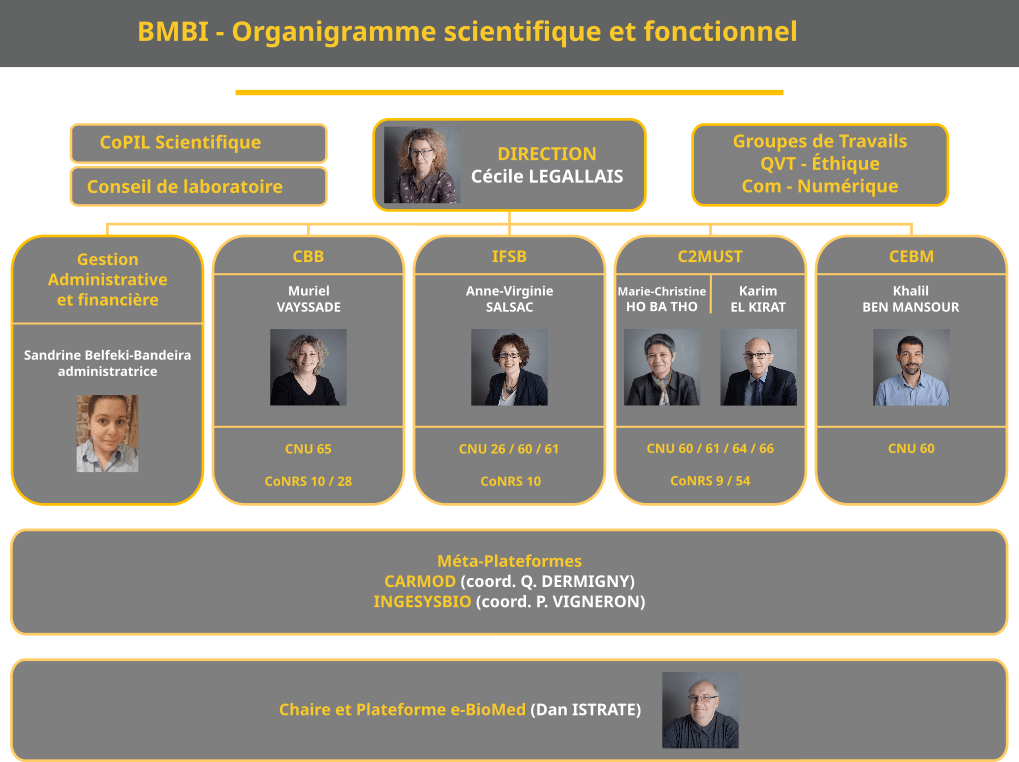
\includegraphics[width=0.6\textwidth]{assets/organigramme-fonctionnel-juillet2025.png}
        \caption{Organigramme du BMBI – \textit{bmbi.utc.fr/annuaire/}}
        \label{fig:organigramme-bmbi}
    \end{figure}

    Le laboratoire BMBI de l'UTC est un centre de recherche qui se concentre sur l'étude de la biomécanique et de la bio-ingénierie, et plus particulièrement sur la mécanique du vivant et l'ingénierie pour la santé. Associé au CNRS depuis 1982, il regroupe depuis plus de 40 ans plusieurs
    disciplines scientifiques telles que la mécanique, la biologie, l'électronique, le traitement du signal, l'informatique, la physique et la biochimie. En tout, il existe plus de 650 documents publiés dans des articles/revues scientifiques, et quasiment 100 thèses soutenues. Il est structuré en plusieurs équipes : Cellules Biomatériaux Bioréacteurs (équipe CBB), Interaction Fluides Structures Biologiques (équipe IFSB), caractérisation et modélisation personnalisée du Système Musculo-Squelettique (équipe C2MUST), et enfin l'équipe BioMov-E (ex CEBM) dans lequel j'ai été affilié durant mon stage.

    L'axe scientifique BioMov-E est né de la fusion entre deux entités complémentaires du BMBI : le Centre d'Expertise de Biomécanique du Mouvement (CEBM) et la chaire EBioMed (Objets Biomédicaux Connectés). Sa thématique de recherche principale porte sur le développement de modèles et de solutions permettant de suivre et d'analyser l'état de santé de l'Homme et de l'animal, d'évaluer sa performance et de prévenir les accidents ou le développement de pathologies.
    
    L'équipe BioMov-E s'appuie sur la plateforme Technologie Sport Santé (TSS) située au centre d'Innovation de l'UTC, qui comprend de nombreux équipements de pointe dédiés à l'analyse du mouvement humain. Des systèmes comme la technologie optoélectronique Hautes Résolutions du Vicon T160 (système de capture de mouvement avec marqueurs), des ergomètres, des plateformes de force, ainsi que des systèmes de test d’effort physique comme le Cosmed K5 sont utilisés pour étudier la biomécanique du mouvement dans divers contextes, allant de la rééducation à la performance sportive.

    TSS est l'une des plateformes les plus complètes en Europe dans le domaine de l'analyse du mouvement humain et a déjà servi de support dans plusieurs projets européens. Elle participe aussi au parcours pédagogique des étudiants de l'UTC, en leur offrant la possibilité de réaliser des stages et des projets de recherche appliqués dans le domaine de la biomécanique du mouvement. 

\section{Présentation de l'équipe BioMov-E}

    Durant le stage, j'étais intégré à l'équipe BioMov-E. Dirigé par mon tuteur de stage M. BEN MANSOUR, j'ai été accompagné par trois autres chercheurs/doctorants : Théophile COCQUEREZ, Julie PROCOPE-MAMERT et Guillaume TOFFOLI. J'étais aussi en contact régulier avec les autres membres de l'équipe BioMov-E lors de réunions. Enfin une autre stagiaire, Yiyang HUANG, effectuait aussi son TN09 sur le projet MoCapIA. À quelques mètres, on a pu échanger sur nos avancées, les méthodes à suivre, les difficultés rencontrées. Son travail concernait plus la poursuite du développement de l'interface utilisateur de l'application MoCapIA, en intégrant les fonctionnalités que je développais. Nous disposions chacun d'un bureau disposé dans un open-space avec les autres membres de l'équipe. Chaque semaine, nous avions une réunion avec M. BEN MANSOUR pour discuter de nos avancements ainsi que des prochaines étapes à suivre, et chaque mois, une réunion avec l'ensemble de l'équipe BioMov-E pour faire le point sur les différents projets en cours et partager nos résultats/difficultés. Le reste du temps, nous étions en autonomie et vraiment libre dans la façon d'accomplir le travail demandé. La méthode appliquée nous a été expliquée en début de stage, sur la manière d'effectuer un travail de rechercher, valider ses choix. Chaque étape commençait par une recherche bibliographique approfondie, et après avoir discuté avec le tuteur des différentes options possibles, nous pouvions commencer le développement. Enfin chaque ajout devait être testé et validé rigoureusement avec les métriques adaptées.

\section{Contexte Scientifique}

    La capture du mouvement (mocap) est un processus en plusieurs étapes : son but est d'extraire les mouvements d'une personne ou d'un objet à partir de données brutes, généralement des vidéos. C'est utilisé dans de nombreux domaines, allant de l'animation 3D dans les films et les jeux vidéos, à l'analyse biomécanique dans le domaine médical et sportif. Pour ça, il faut créer un modèle numérique 3D du mouvement à partir de points caractéristiques. Cette technologie est très utile dans le domaine de la santé comme la rééducation. Elle peut aussi être convoitée pour améliorer ses performances sportives. Avec un modèle 3D recréant le mouvement parfait, la détection du mouvement de l'athlète pourrait lui permettre de se rapprocher du geste parfait. 
    
    Traditionnellement, cela se faisait en utilisant des systèmes de capture de mouvement basés sur des marqueurs physiques attachés au corps du sujet. Ces marqueurs sont suivis par plusieurs caméras haute vitesse pour enregistrer leurs positions dans l'espace 3D, comme le système Vicon T160. Il dispose d'environs 40 caméras opto-électroniques à haute vitesse (jusqu'à 300 images par secondes) capables de suivre avec une grande précision les marqueurs réfléchissants placés sur le corps du sujet.

    Mais ces systèmes présentent plusieurs inconvénients majeurs. Ils sont coûteux, nécessitent un équipement spécialisé et une installation complexe. De plus, le port de marqueurs peut être inconfortable pour les sujets et peut influencer leur mouvement naturel. Ces limitations empêchent une adoption plus large, et notamment dans les domaines de la santé et du sport (comme mentionné précédemment) malgré leur fiabilité de l'ordre du dixième de millimètres. La plateforme BioMov-E dispose d'un tel système, le Vicon T160, qui s'avéra très utile pour mesurer et valider la précision de notre système en cours de développement introduit dans la prochaine section.

    Face à ces défis, une nouvelle approche de capture de mouvement \textbf{sans marqueurs} (markerless) a émergé. Cette méthode, entraînée par les avancées en intelligence artificielle, fait l'objet de plusieurs recherches récentes. En 2019, une entreprise canadienne \textit{Theia Markerless} a développé une technologie de ce genre. Crée et validée par des chercheurs, cette solution haut de gamme est certes précise, mais se rapproche finalement du coût et de la complexité des systèmes avec marqueurs (licence et matériels coûteux). D'autres équipes de recherches travaillent sur cette technologie, comme l'équipe CAMERA (Centre for the Analysis of Motion, Entertainment Research and Applications) de l'université de Bath au Royaume-Uni \cite{BATHResearch}. En partenariat avec l'Association de Bobsleigh britannique, l'équipe met au point un système de capture de mouvement markerless à l'aide de neuf caméras. Leurs objectifs sont comparables aux nôtres (voir section suivante).

    
\section{Objectif du stage}

    Notre but va donc être de développer un système de capture de mouvement \textbf{sans marqueurs} (markerless) en utilisant des techniques avancées de vision par ordinateur et d'intelligence artificielle. Ces techniques permettent de ne plus avoir besoin de marqueurs physiques, remplacé par des marqueurs virtuels détectés automatiquement dans les images. Le reste du processus – calibration, triangulation, reconstruction 3D - reste similaire. Cette approche offre plusieurs avantages : elle est plus flexible, moins coûteuse et permet une capture de mouvement plus naturelle. Cependant, elle présente aussi des défis techniques importants, car remplacer les marqueurs physiques par des marqueurs virtuels implique de nouvelles contraintes et imprécisions.
    \begin{figure}[ht]
    \centering
    \begin{subfigure}{0.48\textwidth}
        \centering
        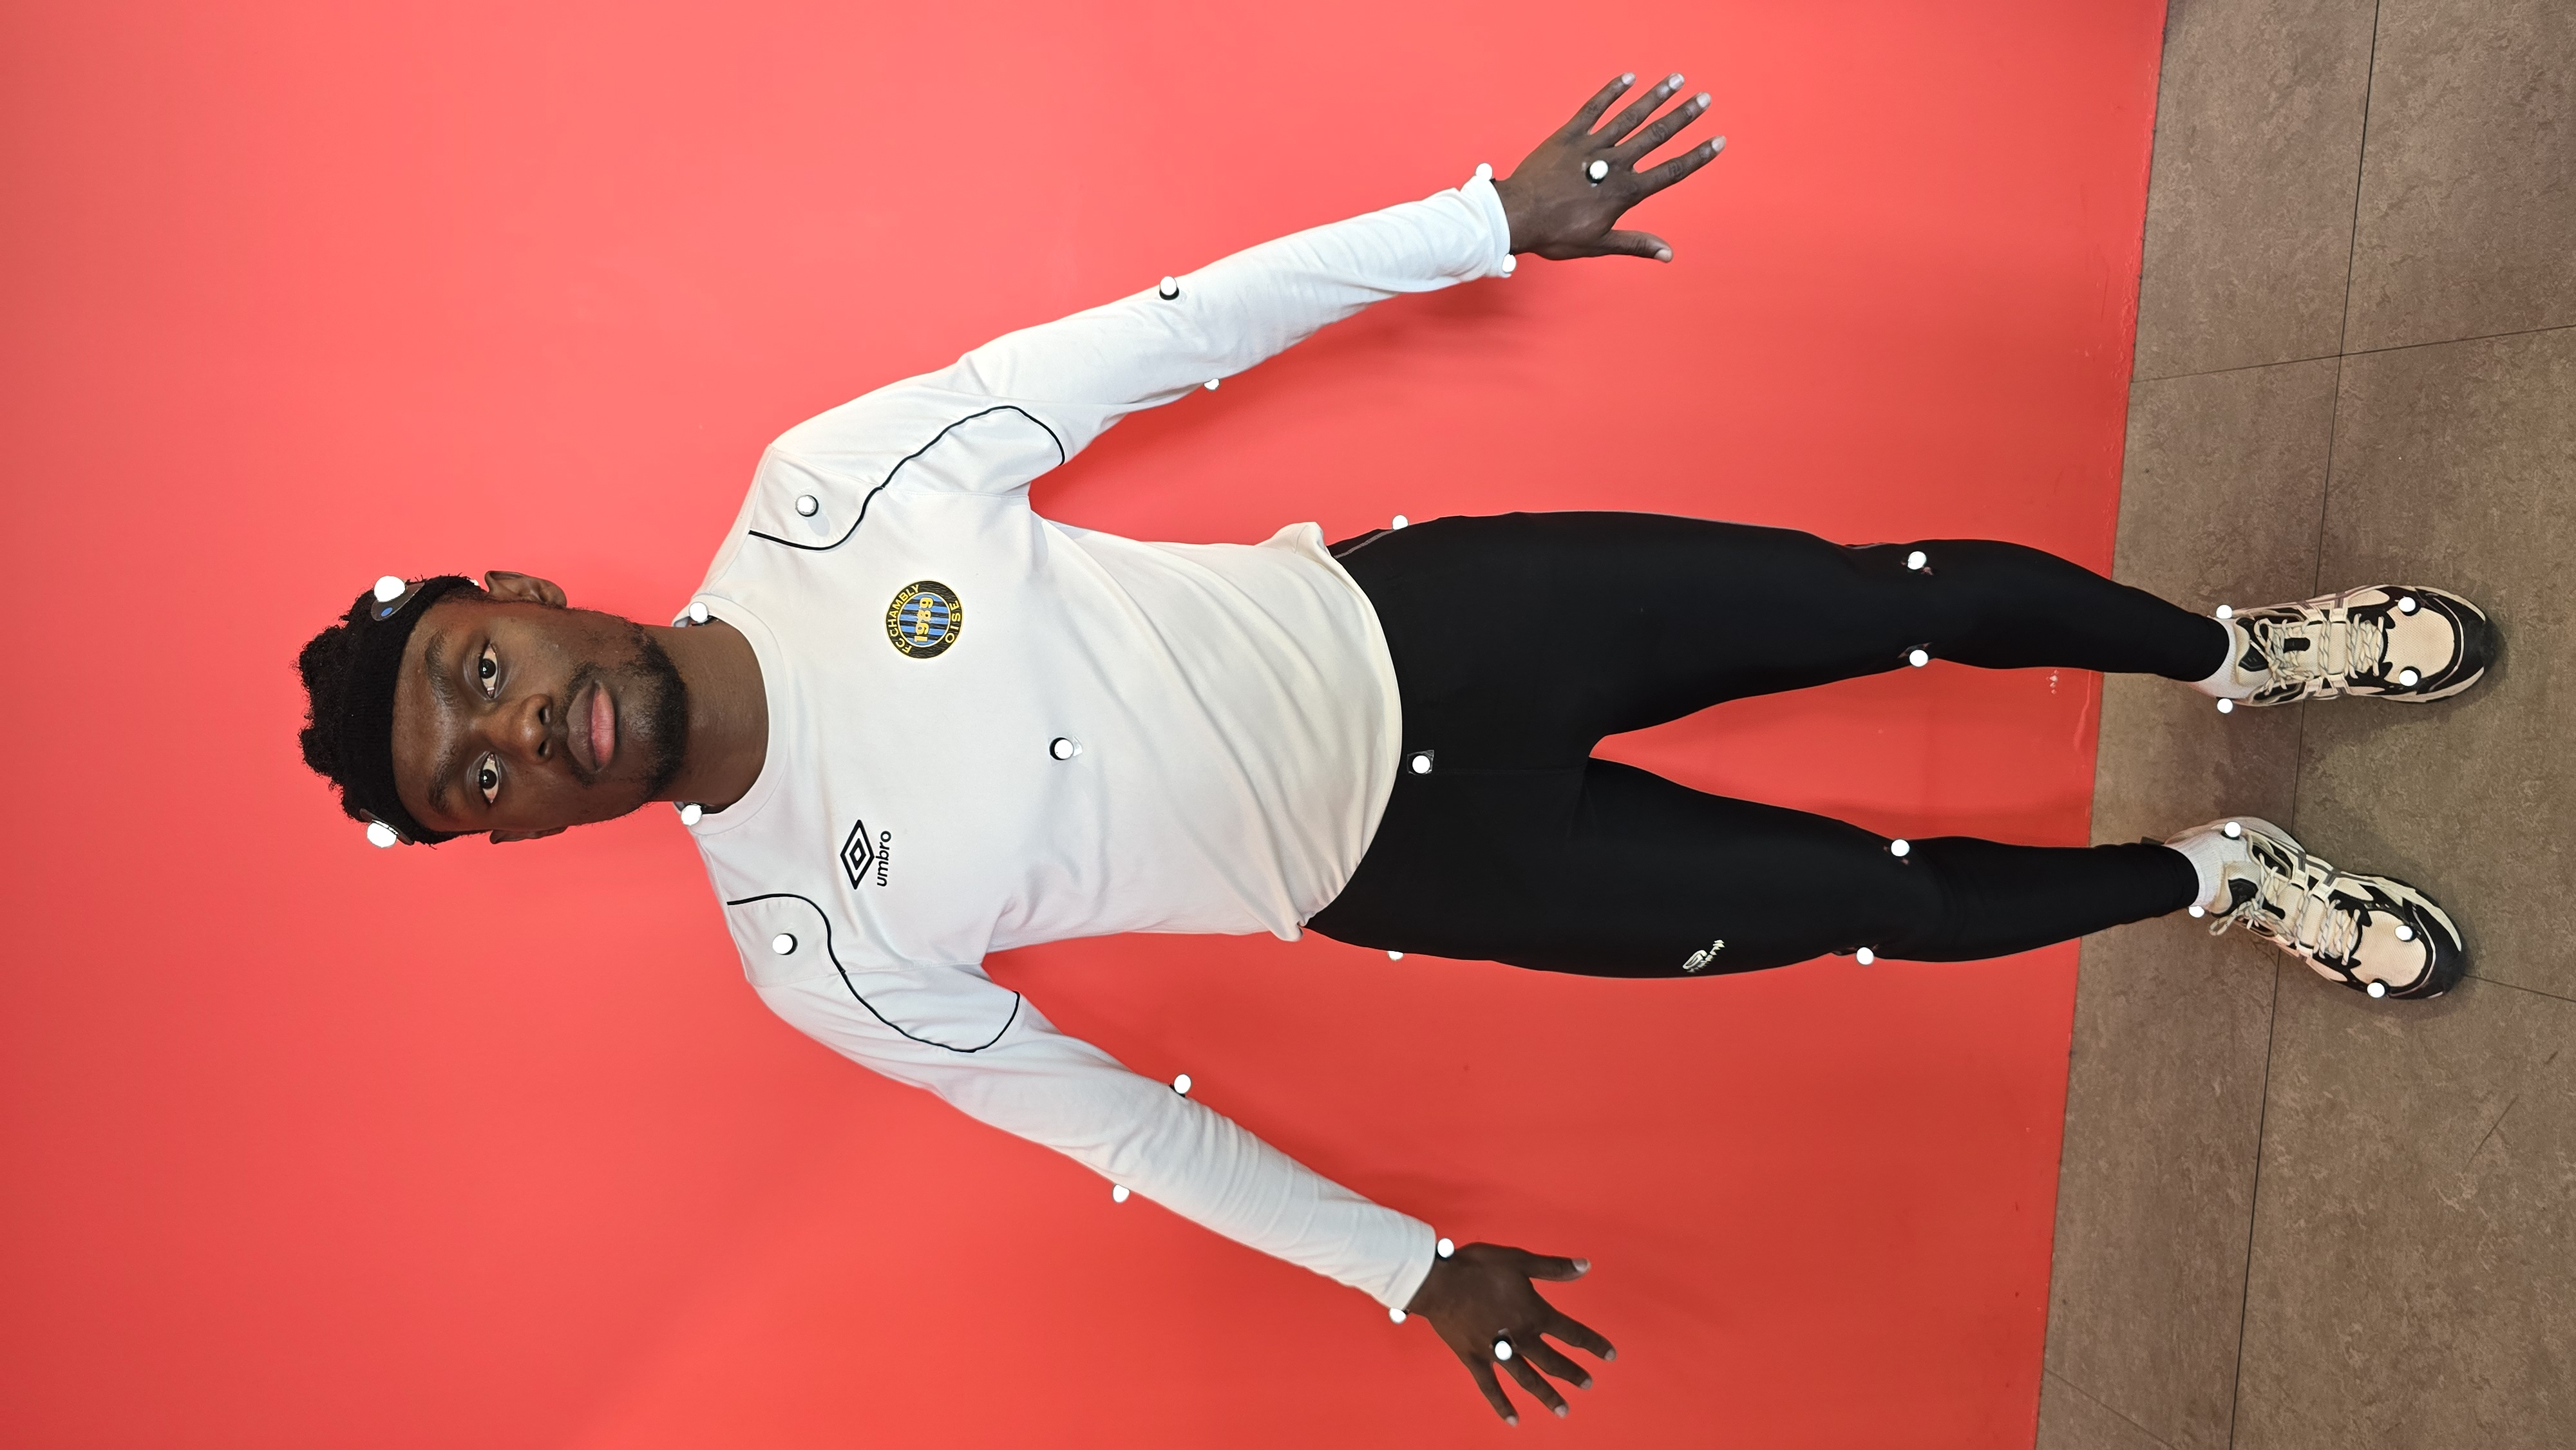
\includegraphics[width=\linewidth, angle=-90]{assets/Capture d'écran process/general/dorian_viconmarkers.jpg}
        \caption{Avec marqueurs}
        \label{fig:vicon-markers}
    \end{subfigure}% <--- Le signe % ici annule l'espace invisible
    \hfill
    \begin{subfigure}{0.48\textwidth}
        \centering
        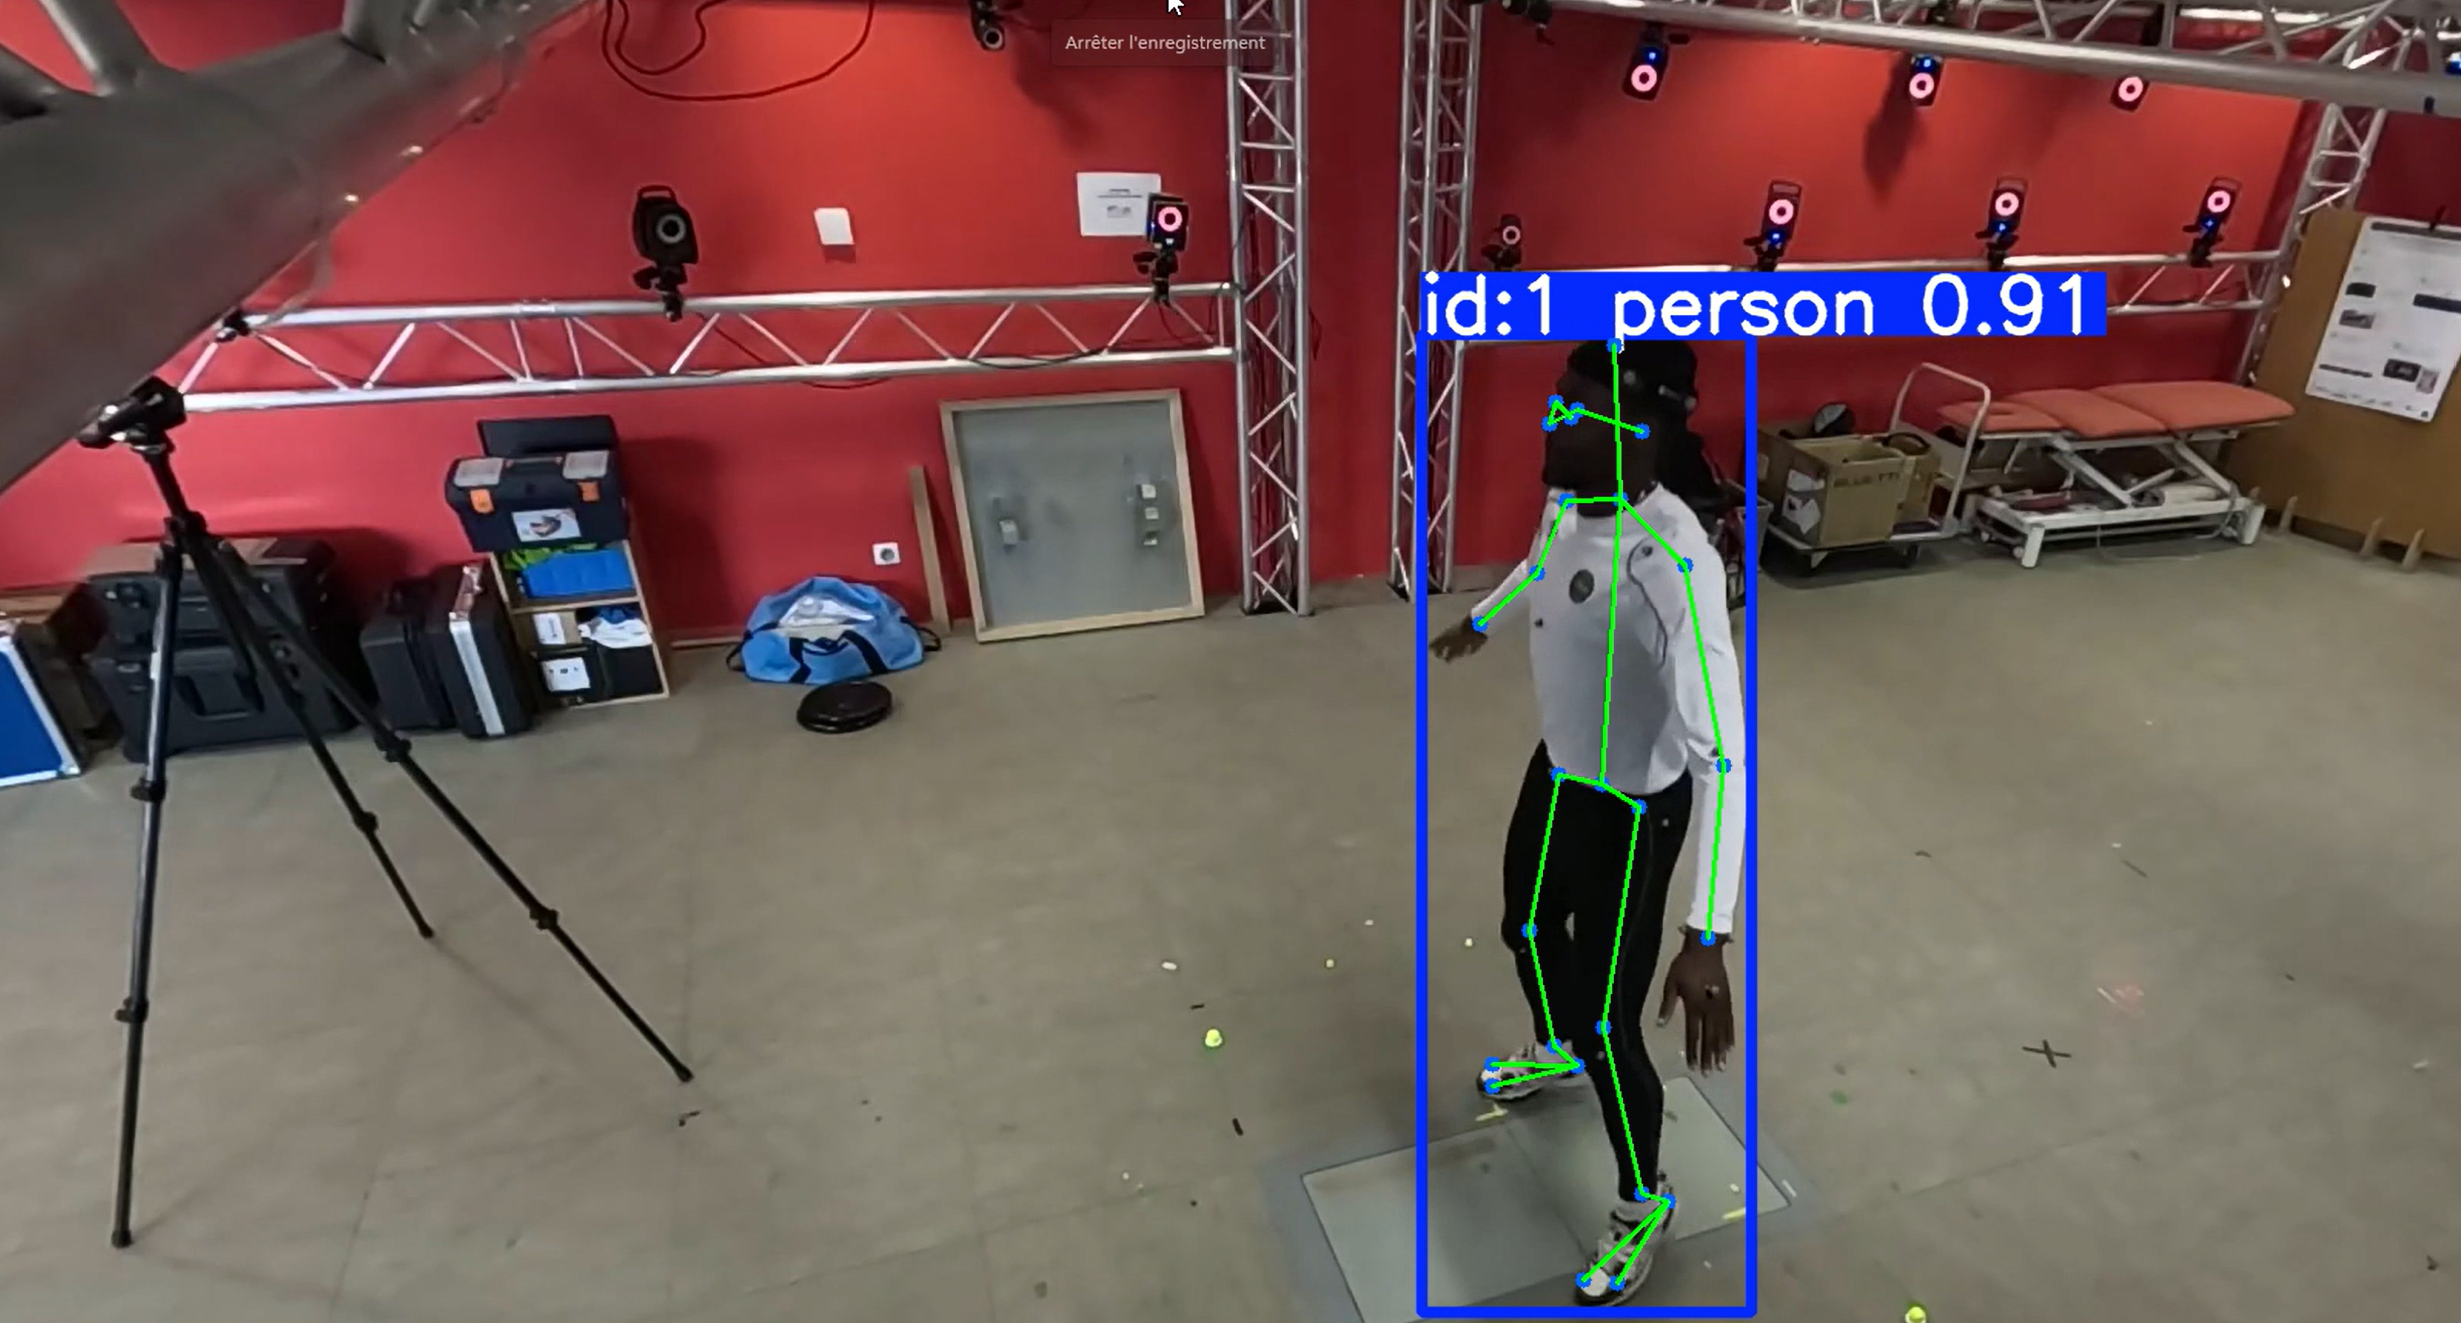
\includegraphics[width=\linewidth]{assets/Capture d'écran process/general/dorian_mocapmarker.png}
        \caption{Sans marqueurs}
        \label{fig:mocap-markers}
    \end{subfigure}
    \caption{Comparaison entre les systèmes de capture de mouvement avec et sans marqueurs}
    \label{fig:mocap-comparaison}
\end{figure}
    
    Durant les quatre derniers semestres, quatre stagiaires ont déjà effectué leur stage dans le cadre de ce projet. Les fonctions de bases ont été instaurées dès les premiers stagiaires comme la calibration, la synchronisation, la triangulation ainsi qu'un Ui (User Interface). L'ajout de fonctionnalités plus avancées autour de l'Ui a été instauré par le dernier stagiaire. L'objectif principal de mon stage est d'identifier la provenance des erreurs restantes afin d'améliorer la robustesse et la précision de la reconstruction 3D. Le but est de se rapprocher d'une précision et d'une capacité d'analyse biomécanique comparable à celle des systèmes avec marqueurs physiques comme le Vicon T160 et permettre l'utilisation en milieu clinique ou sportif.

    Dans le cadre d'un stage en \textbf{recherche}, il est aussi crucial de prendre en compte l'étendue de la littérature scientifique existante sur le sujet afin d'identifier de nouvelles approches et d'améliorer le système en général. Ce type de stage implique aussi une part importante de justification scientifique des choix techniques appliqués ou même rejetés.





\section{Déroulement du stage}
    Le stage s'est déroulé sur une période de 6 mois, de septembre 2025 à février 2026 avec deux semaines de fermeture du laboratoire durant les fêtes de fin d'année (du 20 décembre au 2 janvier).

    Même si le travail de programmation a représenté une part importante du stage, beaucoup de recherche et phases de test ont permis de rendre ce stage enrichissant dans plusieurs domaines. La compréhension du côté mathématique du processus a été aussi vraiment important pour pouvoir espérer améliorer la précision du système.

    Durant les deux premières semaines, il a fallu s'imprégner du contexte scientifique et technique du projet. Accompagné par le précédent stagiaire, on a d'abord, avec ma collègue, pris en main l'interface utilisateur qui permettait de gérer les différentes étapes de la capture de mouvement. On a pris connaissance aussi du "hardware" nécessaire pour le processus de capture, notamment les caméras, leur application, les différents damiers de calibration. En une semaine, on a pu maîtriser l'ensemble du processus, de l'acquisition des vidéos jusqu'aux données 3D et leur reconstruction dans l'espace. Ensuite, il a fallu consulter les anciens rapports, documents techniques et les articles scientifiques dans le domaine pour saisir l'ensemble des enjeux et défis du projet. En deux semaines, les fonctions principales du code ont été comprises, et des pistes d'amélioration ont été identifiées.

    Par la suite, une grosse période a été accordée à la recherche bibliographique. Cela s'est avéré être très utile surtout pour l'aspect mathématique, et m'as permis de mieux comprendre le fonctionnement interne de chaque étape et d'identifier les pistes d'améliorations.
    \chapter{Présentation du Projet MoCapIA}

    Maintenant, nous allons présenter le projet MoCapIA en détail, en expliquant les piliers mathématiques sur lesquels il repose, son fonctionnement général. Nous parlerons aussi de l'historique du projet, les travaux accomplis par les précédents stagiaires en détail ainsi que les outils et technologies.

\section{Le processus MoCapIA}
    
    D'après sa définition, la capture de mouvement (motion capture en anglais, parfois abrégé en mocap) est une technique permettant d'enregistrer les positions et rotations d'objets ou de membres d'êtres vivants, pour en contrôler une contrepartie virtuelle sur ordinateur (caméra, modèle 3D ou avatar). Dans notre système, on se focalise sur l'obtention du modèle 3D d'un être humain.
    Il y a 3 étapes principales : la calibration, la détection 2D du corps humain et la reconstruction 3D. Voici un schéma qui résume le projet MoCapIA et son fonctionnement général \textbf{au début du stage} :
    \begin{figure}[H]
        \centering
        
\includegraphics[width=0.8\textwidth]{assets/Capture d'écran process/general/synthèseMOCAPIA.drawio.png}
        \caption{Schéma récapitulatif du fonctionnement général de début de stage}
        \label{fig:fonctionnement_mocapia_debut}
    \end{figure}
    
    \subsection{Partie 1 - Mise en place des caméras et de la calibration}

        Pour capturer le mouvement, nous utilisons 2 à 4 caméras GoPro (précisions dans la partie Outils et Technologies). Ces caméras sont placées autour de la zone de capture de façon à qu'elles aient dans leurs champs de vision une zone commune. Cette zone est l'endroit où l'utilisateur va effectuer son mouvement. Chaque caméra est fixée et ne doit pas bouger durant toute l'expérience (calibration + capture du mouvement). Elles doivent aussi utiliser le même réglage (résolution, fréquence d'images, angle de vue) et doivent être synchronisées entre elles. Pour ça on utilise l'application GoPro qui permet de synchroniser un timecode commun sur les caméras.

        \begin{figure}[H]
            \centering
            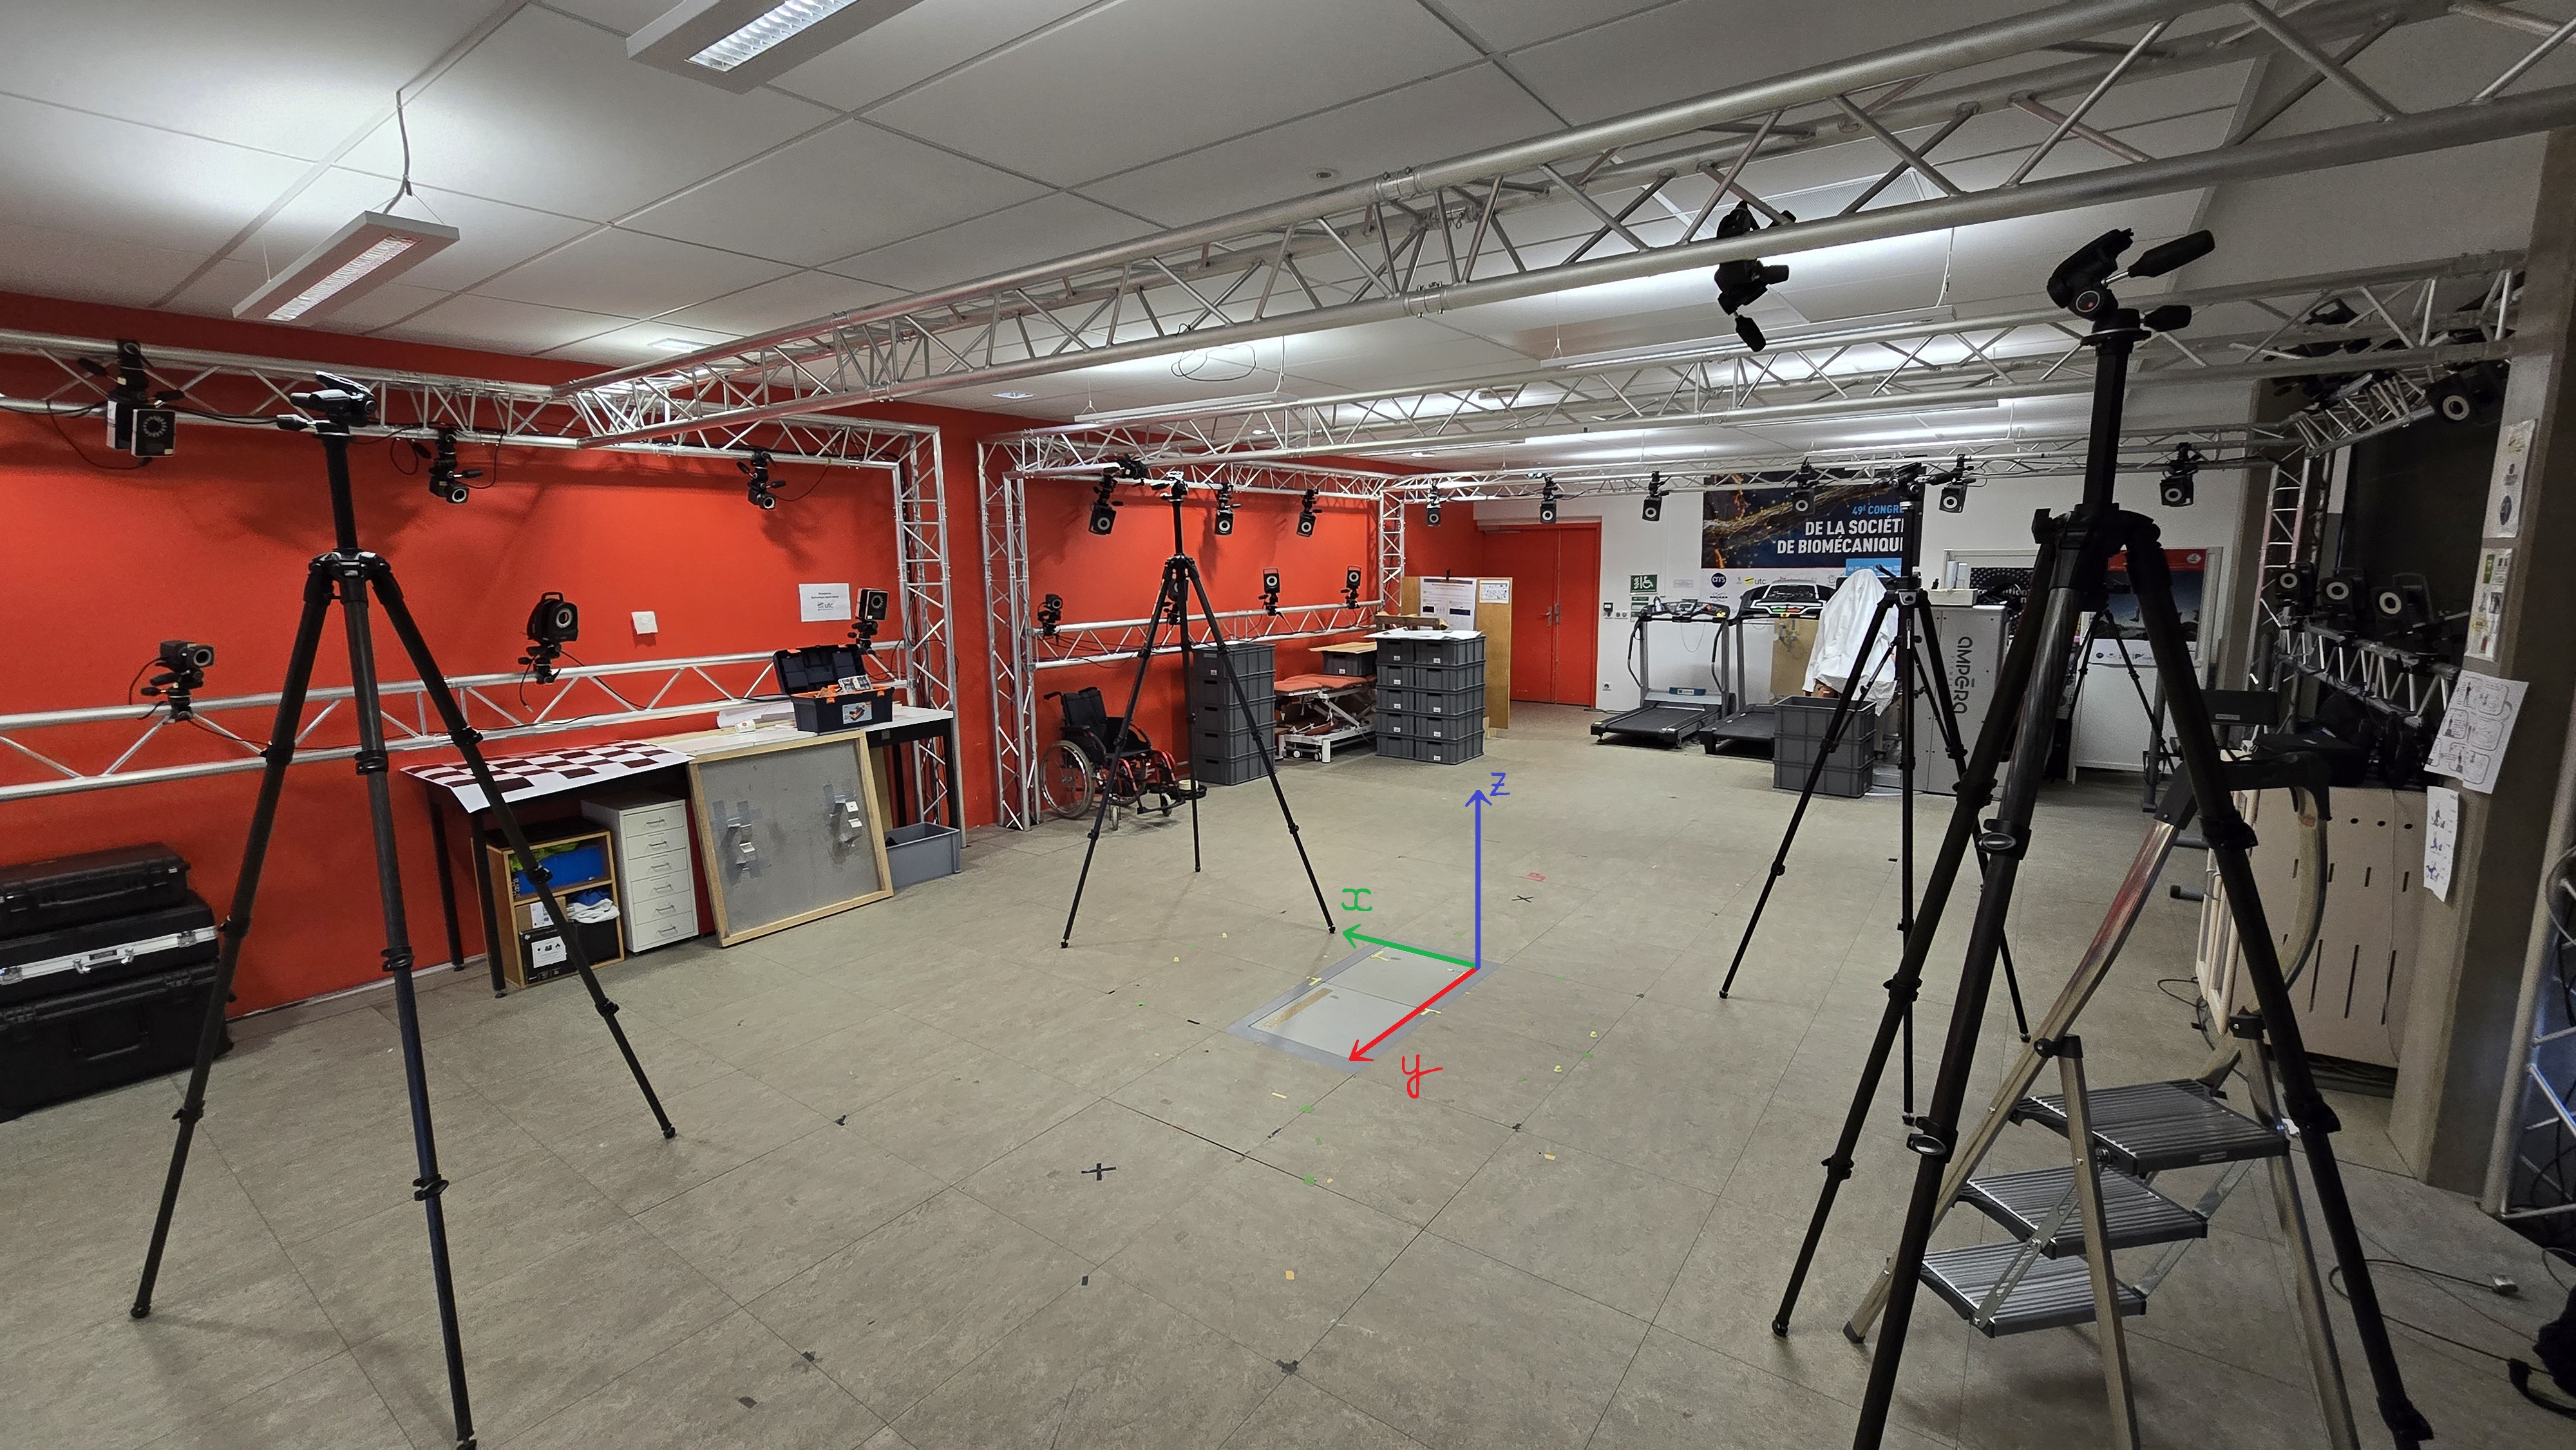
\includegraphics[width=0.8\textwidth]{assets/Capture d'écran process/general/vue trepied.jpg}
            \caption{Mise en place des caméras sur trépied autour de la zone de capture}
            \label{fig:setup_cameras}
        \end{figure}
        Pourtant, avant de capturer le mouvement, on a besoin de calibrer les caméras ce qui est obligatoire avant de vouloir trianguler et obtenir des points 3D. À des fins de compréhension, il est important d'introduire le principe de calibration intrinsèque et extrinsèque \cite{Calibrage}.
        Commençons avec la \textbf{calibration intrinsèque}. Elle consiste à déterminer les paramètres \textbf{internes} à la caméra qui influencent la formation de l'image. Ces paramètres sont fixes donc une fois calculés, ils peuvent être stockés et gardés tant qu'on utilise la même caméra.
        Ces paramètres sont représentés par une matrice $K$ de cette forme :
        $$
        K = \begin{bmatrix}
        f_x & 0 & c_x \\
        0 & f_y & c_y \\
        0 & 0 & 1
        \end{bmatrix}$$
        où :
        \begin{description}
            \item[$f_x$, $f_y$] la focale de la caméra en pixels selon $x$ et $y$
            \item[$c_x$, $c_y$] sont les coordonnées du point d’origine du repère (projection du centre optique sur le plan image)
        \end{description}
        La \textbf{calibration extrinsèque}, quant à elle, définit la position et l'orientation de la caméra dans le repère monde. Les paramètres sont représentés par une matrice de rotation $R \in \mathcal{M}_{3,3}(\mathbb{R})$ et un vecteur de translation $t$. Ces paramètres doivent être recalculés à chaque fois que la caméra est déplacée :
        $$
        [R|t]= \begin{bmatrix}
        r_{11} & r_{12} & r_{13} & t_x \\
        r_{21} & r_{22} & r_{23} & t_y \\
        r_{31} & r_{32} & r_{33} & t_z
        \end{bmatrix} 
        $$ \ref{fig:calibration_cam}
        En appliquant cette matrice $P$ à un point 3D $(X,Y,Z)$ dans le repère monde, on obtient les coordonnées 2D $(u,v)$ dans le repère caméra. Au final, la matrice de projection $P$ de chaque caméra s'obtient en combinant les paramètres intrinsèques et extrinsèques :
        $$
        P = K [R|t]
        $$
        Ces matrices seront utilisées plus tard pour la triangulation des points 3D.
        Dans notre projet l'ensemble de ces informations sont stockées dans un fichier $hdf5$, un format de fichier conçu pour stocker et organiser des données.
        \begin{figure}[H]
            \centering
            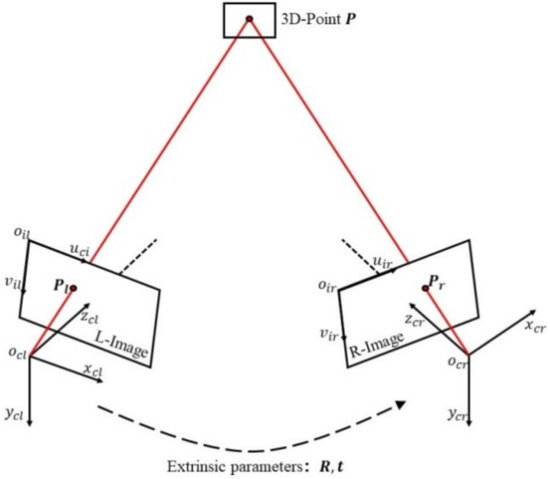
\includegraphics[width=0.7\textwidth]{assets/Capture d'écran process/general/calibration.jpg}
            \caption{Calibration extrinsèque des caméras (cf. \cite{calibraExtrinsic})}
            \label{fig:calibration_cam}
        \end{figure}
        Comme le montre cette figure \ref{fig:calibration_cam}, le repère monde est initialement défini comme le repère 3D de la caméra 1 (ce référentiel sera amené à être changé plus tard).

        \subsection{Estimation de Pose 2D}

        L'estimation 2D du corps humain est l'autre étape importante avant de pouvoir obtenir le modèle 3D final et introduit un aspect essentiel du système : l'Intelligence Artificielle. En effet, comme le projet MoCapIA est un système \textbf{markerless} (sans marqueurs), on identifie les points clés du corps humain grâce à des modèles pré-entraînés. Il en existe plusieurs, chacun ont leurs spécificités, avantages et inconvénients (cette étude a été mené par un ancien stagiaire, voir ...). Nous utilisons une combinaison de deux modèles : YOLO et RTMPose. YOLO (You Only Look Once) est un modèle de détection d'objets en temps réel qui permet de localiser rapidement un objet (ici le corps humain) dans une image. Il assigne à chaque image une carte de classification en fonction des probabilités de présence d'un objet et génère une \textbf{bounding box} (boîte englobante). Il est doté d'un algorithme de tracking qui permet de garder la même bounding box sur le bon sujet durant toute la vidéo.
        \begin{figure}[H]
            \centering
            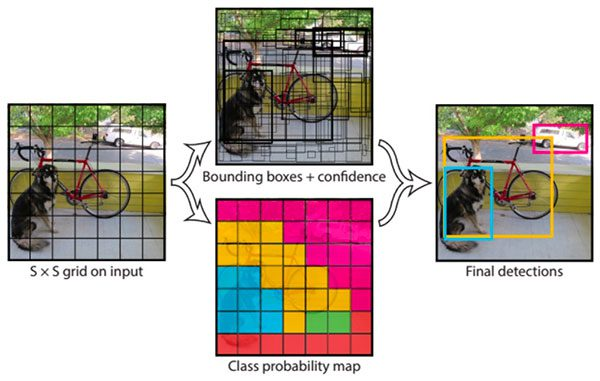
\includegraphics[width=0.7\textwidth]{assets/Capture d'écran process/general/yolo.jpg}
            \caption{Fonctionnement de YOLO (cf. \textit{octo.com})}
            \label{fig:yolo}
        \end{figure}
        Cette étape permet de découper l'image pour ne garder que la partie contenant le corps humain. Ensuite, on utilise le deuxième modèle RTMPose qui est un modèle d'estimation de pose basé sur des (CNN). Il permet de détecter les points clés du corps humain en 2D dans l'image en générant une carte de chaleur, représentant  leur probabilité de présence. Entrainé sur différents squelettes, nous utilisons le modèle Halpe26 qui détecte 26 points clés du corps humain. Les points clés sont stockés dans un fichier .JSON.
        \begin{figure}[H]
            \RawFloats
            \centering
            % --- Figure de Gauche ---
            \begin{minipage}[t]{0.3\textwidth}
                \centering
                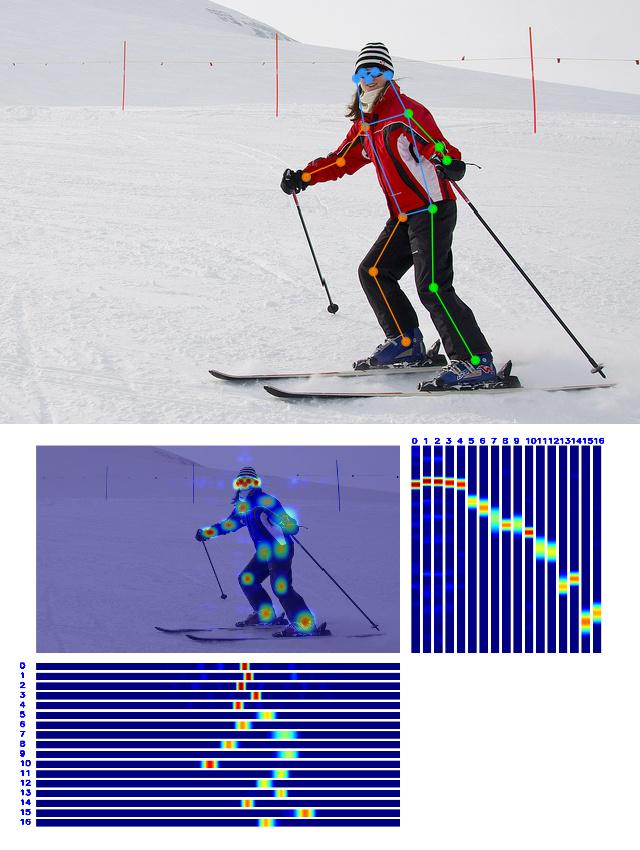
\includegraphics[width=\linewidth]{assets/Capture d'écran process/general/rtmpose.png}
                \caption{Fonctionnement de RTMPose (cf. \href{https://github.com/open-mmlab/mmpose/releases/tag/v1.3.2}{GitHub MMPose})}
                \label{fig:rtmpose}
            \end{minipage}
            \hfill % Espace vital entre les deux
            % --- Figure de Droite ---
            \begin{minipage}[t]{0.5\textwidth}
                \centering
                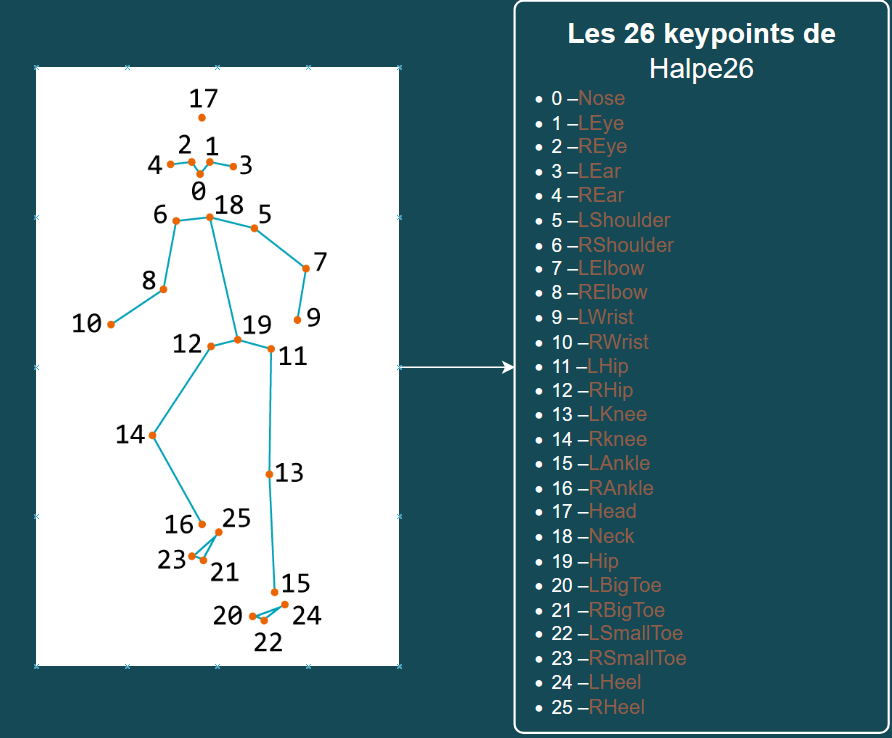
\includegraphics[width=\linewidth]{assets/Capture d'écran process/general/halpe26.png}
                \caption{Modèle Halpe26}
                \label{fig:halpe26}
            \end{minipage}
        \end{figure}
        
    \subsection{Reconstruction 3D}

        Nous disposons maintenant les informations nécessaires pour reconstruire le modèle 3D du corps humain. La première partie de cette reconstruction 3D utilise OpenCV pour trianguler les points 3D à partir de deux premières caméras. Avec un point 2D et les résultats de la calibration de la caméra concernée, on peut tracer une droite dans l'espace 3D partant du centre optique $C$ et passant par le pixel $(u,v)$ projeté en 3D grâce à la matrice intrinsèque $K$ et extrinsèque $R$,$t$ de la caméra :
        $$
        C = -R^{T}t \qquad \text{et} \qquad d = R^{T} \left( K^{-1} \begin{bmatrix} u \\ v \\ 1 \end{bmatrix} \right)
        $$      
        En théorie, pour obtenir la position 3D exacte du point, il suffit d'utiliser une deuxième caméra pour tracer une seconde droite et retrouver l'intersection entre elles. Évidemment dans la réalité les droites ne se coupent pas exactement à cause des erreurs de détection 2D et de calibration. On utilise donc la méthode DLT (Direct Linear Transform) pour minimiser la distance entre les deux droites et obtenir une estimation du point 3D. Disposant de $N$ caméras, on peut générer des candidats pour chaque paire de caméra (figure \ref{fig:triangulation_dlt}). On utilise donc une méthode de \textbf{binning} pour regrouper les candidats dans différents intervalles et renvoie la moyenne de l'intervalle ayant le plus de candidats. Cette méthode permet de réduire l'impact des erreurs de détection et assure une trajectoire 3D plus stable.
        \begin{figure}[H]
            \centering
            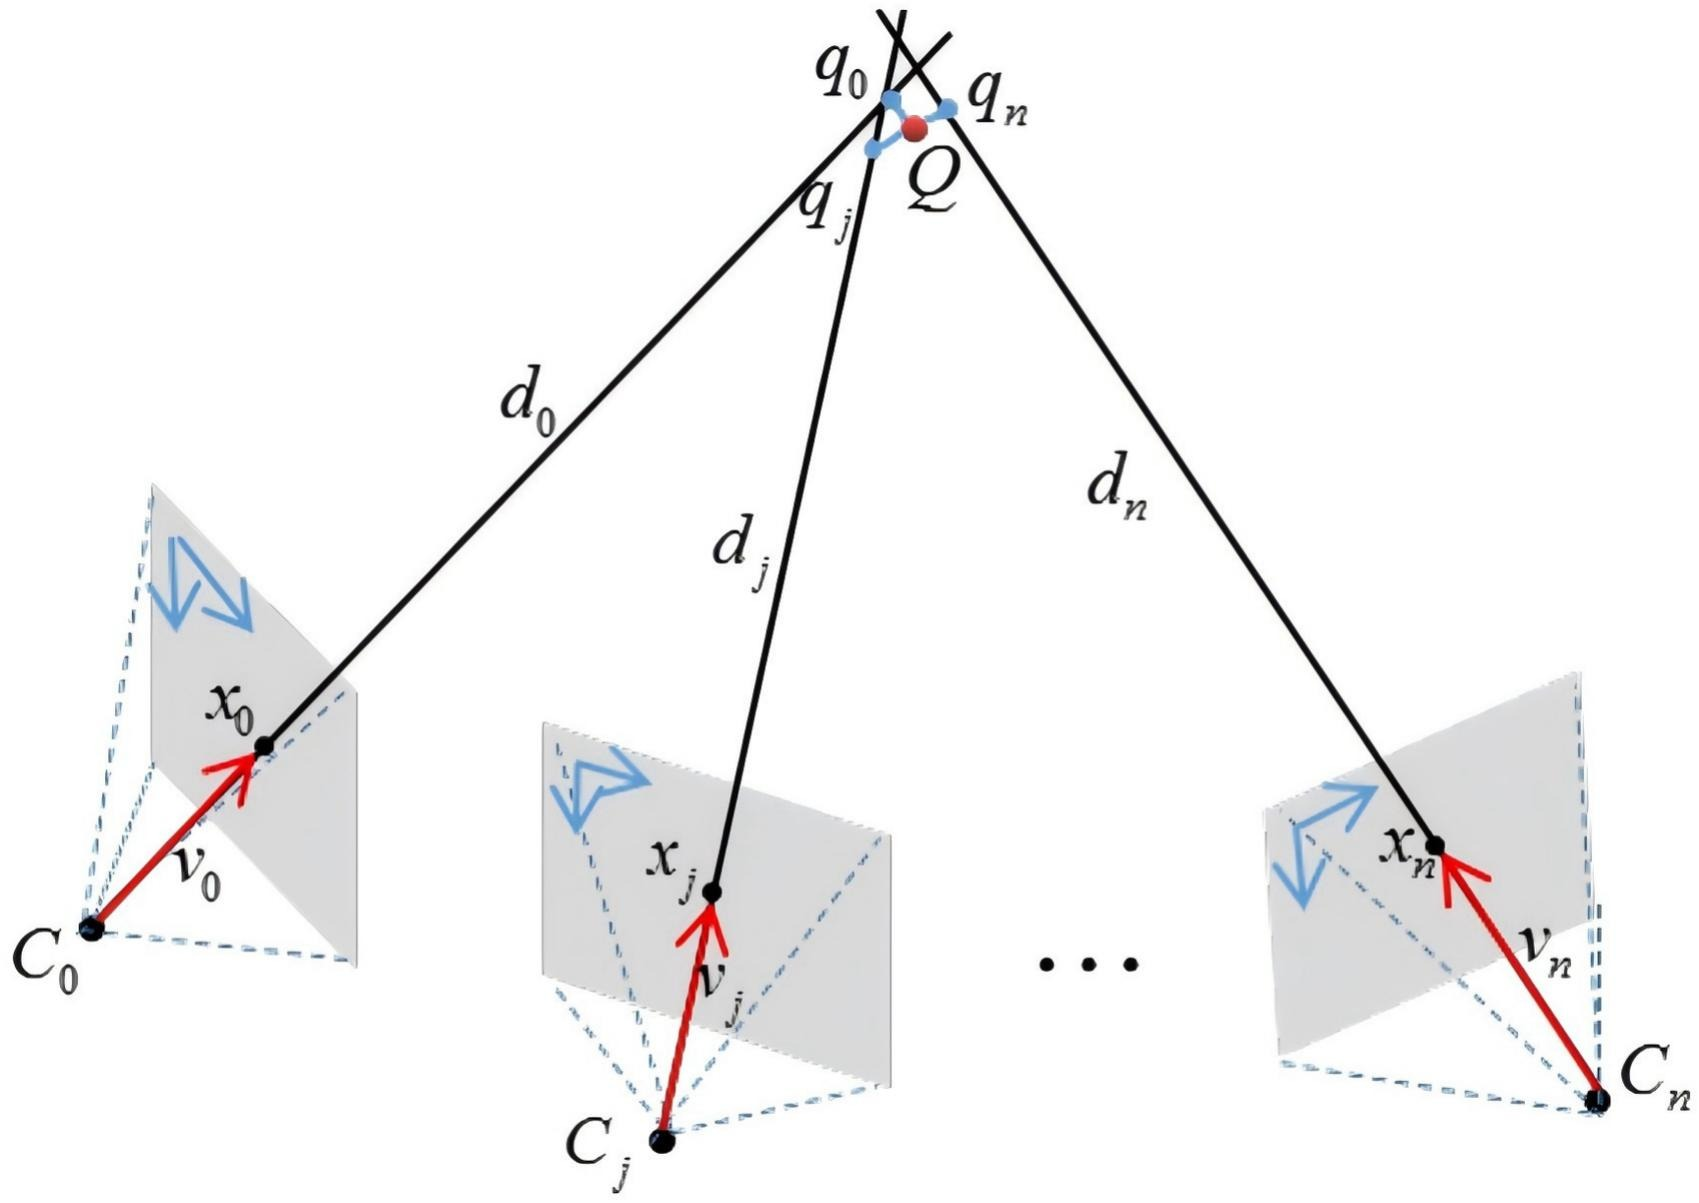
\includegraphics[width=0.8\textwidth]{assets/Capture d'écran process/general/DLT.jpg}
            \caption{Principe de triangulation par DLT (cf. \cite{OrthogonalProjections})}
            \label{fig:triangulation_dlt}
        \end{figure}

        Enfin les coordonnées 3D sauvegardées dans un fichier .CSV sont placés dans le repère monde initial (celui de la caméra 1). Pour mieux pouvoir visualiser et analyser les données, nous devons transformer ce repère dans celui du laboratoire. Pour ça on utilise une transformation rigide (rotation + translation) calculée à partir de points de références 0, X et Y cliqués sur chaque vue des caméras.
        \begin{figure}[H]
            \centering
            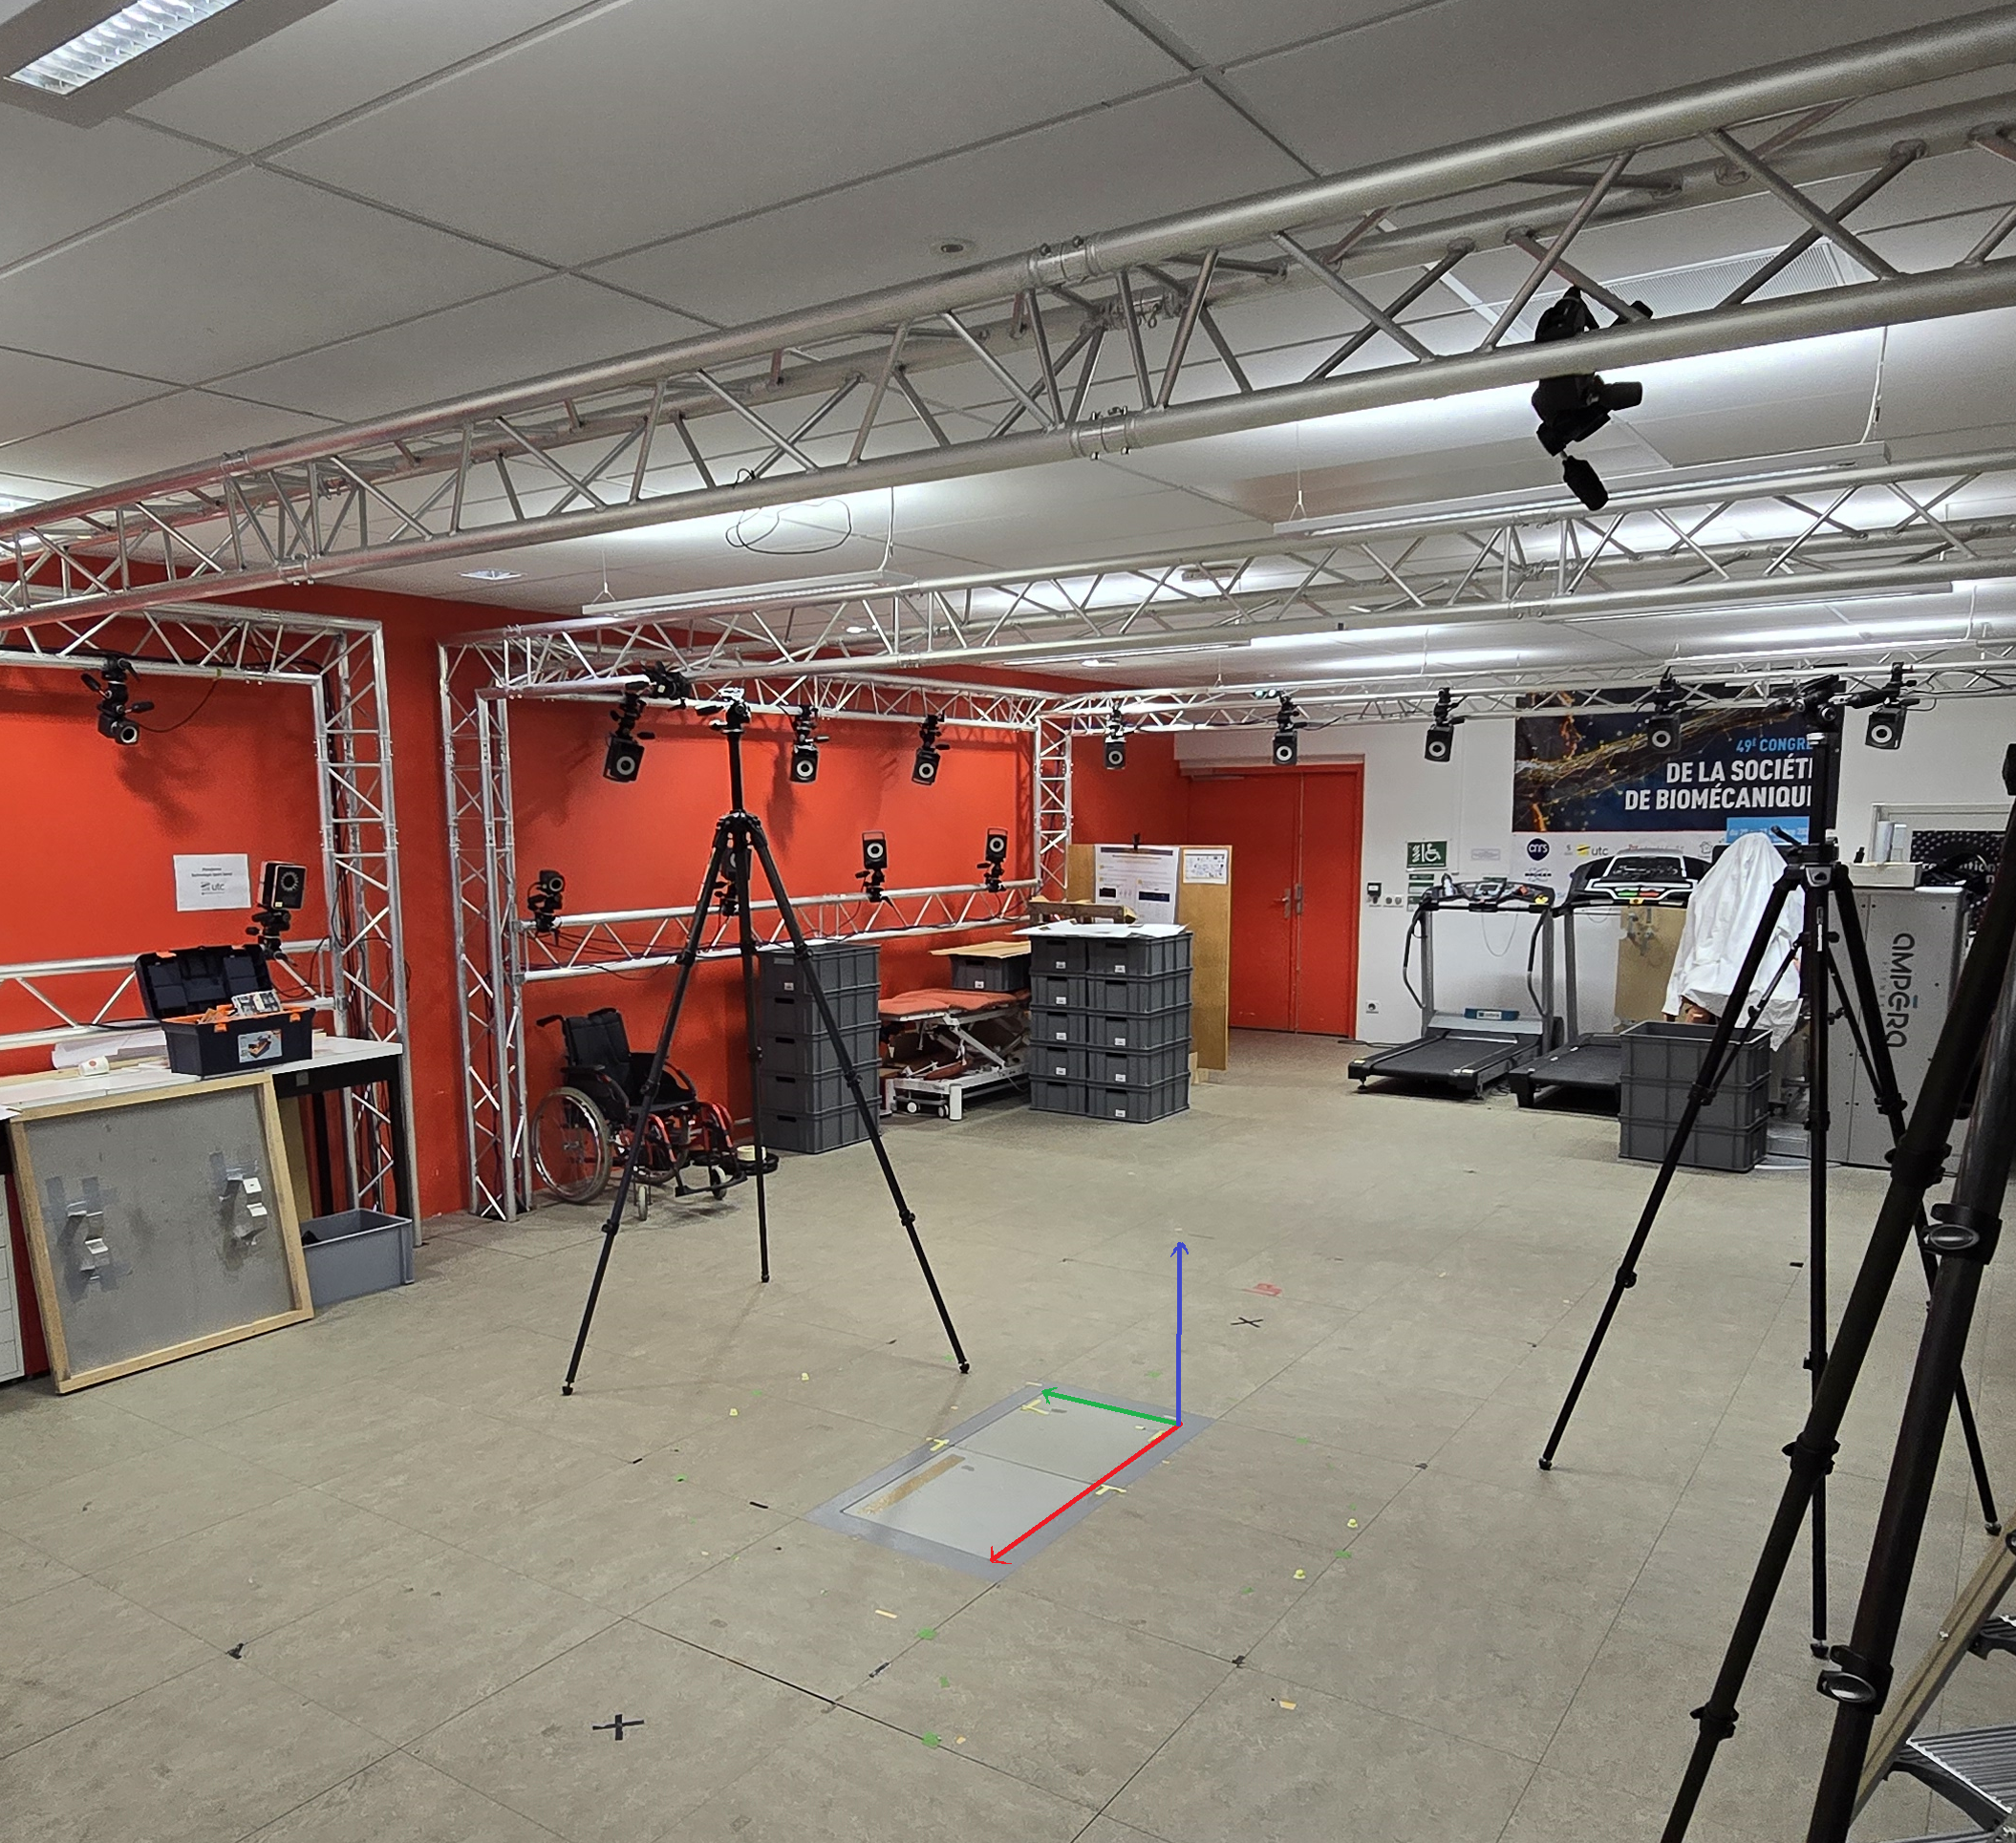
\includegraphics[width=0.8\textwidth]{assets/Capture d'écran process/general/change_ref.png}
            \caption{Changement de repère}
            \label{fig:change_ref}
        \end{figure}

    \subsection{Interface graphique}
        
        Pour l'ensemble de ces étapes, on utilise une interface graphique développée en Python à l'aide la bibliothèque PyQt5. Il permet une utilisation \textbf{user-friendly} ce qui est essentielle pour une future utilisation en milieu clinique ou sportif. En plus de rendre facile la mise en place de la calibration, l'estimation 2D et la triangulation, l'interface permet d'ajouter d'autres fonctionnalités intéressantes :
        \begin{itemize}
            \item \textbf{Structuration des expériences :} Lors de chaque nouvelle expérience, il est possible de créer un nouveau projet, et d'y ajouter un ou plusieurs sujets. Enfin, on peut attribuer à chaque sujet plusieurs sessions de capture.
            \item \textbf{Visualisation du modèle 3D :} Une fois la triangulation terminée, on peut visualiser le fichier CSV (de coordonnées 3D) directement dans l'interface graphique. On a la possibilité d'afficher la distance entre deux points du modèle ou l'angle entre 3 points pour valider ou non la qualité du modèle et permettre l'analyse biomécanique.
            \item \textbf{Lecture des logs :} Durant chaque étape du processus MoCapIA, des logs sont générés pour informer l'utilisateur de l'état d'avancement et d'éventuelles erreurs. L'interface permet de consulter ces logs facilement.
            \item \textbf{Gestion des caméras :} L'interface permet de gérer les caméras GoPro, notamment en choisissant les caméras connectées et leurs réglages (résolution, fréquence d'images, angle de vue).
        \end{itemize}

\section{Historique}

        Comme mentionné précédemment, le projet MoCapIA a été initié en 2023 au semestre d'automne. Jusqu'à maintenant, quatre stagiaires ont travaillé sur le projet, chacun apportant des contributions significatives à son développement. Voici un résumé des travaux accomplis par chaque stagiaire :
        \begin{itemize}
            \item \textbf{Stagiaires 1 et 2 :}
            Les deux premiers stagiaires ont principalement travaillé sur la recherche et l'évaluation des algorithmes et modèles d'IA les plus performants pour réaliser l'estimation de pose 2D en offrant une précision satisfaisante. Même si aucune valeur chiffrée n'a été précisé, le modèle d'IA choisit est considéré comme le plus adapté parmi ceux testés. Les deux critères utilisés pour évaluer les modèles étaient : l'erreur sur les distances et les angles articulaires en comparaison avec le système de référence Vicon, ainsi que la stabilité des points estimés.
            Il existe deux types d'approches dans les algorithmes d'estimation de pose 2D. La première est l'approche \textbf{top-down} qui consiste à d'abord détecter le corps humain dans l'image (généralement avec une bounding box) puis à estimer les points clés à l'intérieur de cette boîte. La seconde approche est \textbf{bottom-up} qui consiste à détecter tous les points clés dans l'image, puis à les regrouper pour former des squelettes complets. Les stagiaires ont conclu que l'approche top-down était plus adaptée pour notre application, car elle offre une meilleure précision et robustesse lors d'expérience avec un faible nombre d'individus tandis que l'approche bottom-up est plus adaptée pour des scènes avec plusieurs. Dans le contexte de MoCapIA, les stagiaires ont privilégié la précision et la robustesse pour un seul sujet. C'est donc l'approche top-down qui a été choisie par l'équipe.
            Parmi les modèles top-down, \textbf{MMPose} est un ensemble d'algorithmes basés sur \textbf{PyTorch}. Accessible via la bibliothèque YOLO, MMPose rassemble plusieurs modèles d'estimation de pose 2D. Après avoir testé plusieurs modèles et en s'appuyant sur une étude menée en 2023 \cite{RTMPose}, les stagiaires ont choisi \textbf{RTMPose} pour sa rapidité et sa précision (cf. \ref{fig:rtmpose_perf}). 
            \begin{figure}[H]
                \centering
                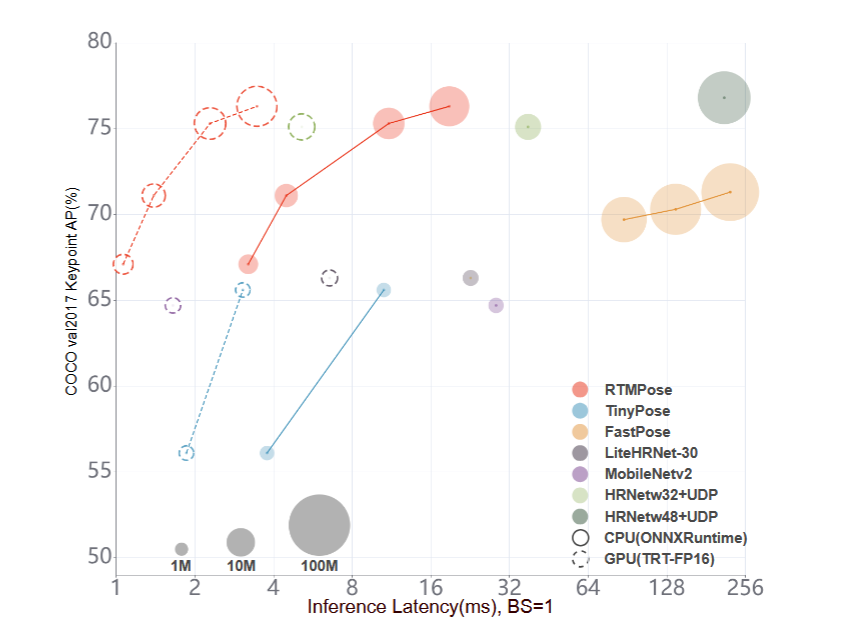
\includegraphics[width=0.8\textwidth]{assets/Capture d'écran process/general/rtmpose_perf.png}
                \caption{Performance de RTMPose comparée à d'autres modèles (cf. \cite{RTMPose})}
                \label{fig:rtmpose_perf}
            \end{figure}
            Il fonctionne en deux étapes : un backbone, suivi d'un détecteur de points clés. Le \textbf{backbone} représente l'architecture principale du modèle (c'est le réseau neuronal convolutif). Il permet l'extraction de caractéristiques sur l'image donc il est en grande partie responsable de la performance du modèle. RTMPose utilise le modèle \textit{ResNet}, qui s'est avéré être  le plus performant. En contrepartie, il est de complexité computationnelle, donc une charge de calcul importante (figure \ref{fig:rtmpose_architecture}). Cette étape est suivie d'un détecteur de points clés qui construit une \textit{heatmap}, représentant les probabilités des positions des points clés. La dernière étape consiste à s'appuyer sur les résultats du backbone et du détecteur pour prédire les positions 2D des points clés du corps humain sous forme de matrice.
            \begin{figure}[H]
                \centering
                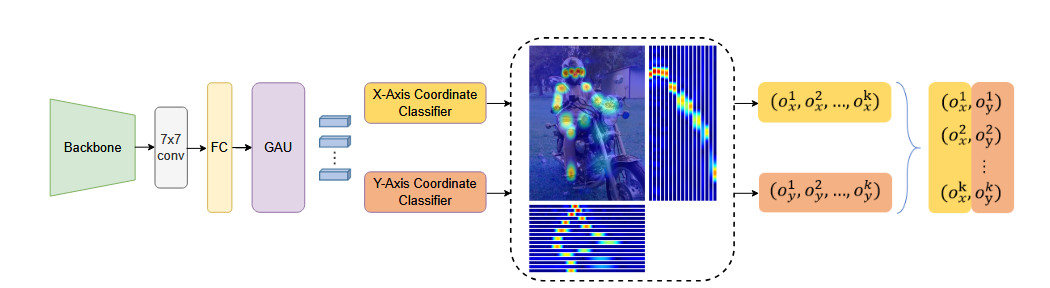
\includegraphics[width=0.8\textwidth]{assets/Capture d'écran process/general/rtmpose_explained.png}
                \caption{Architecture de RTMPose (Han, 2023), un backbone RestNet permet d’extraire les différentes caractéristiques de l’image, puis un détecteur de points clés construit la heatmap des points remarquables du sujet. Ces points sont renvoyés sous la forme d’une matrice (cf. \cite{RTMPose}).}
                \label{fig:rtmpose_architecture}
            \end{figure}
            \item \textbf{Stagiaire 3 :} Durant le semestre A24, le troisième stagiaire a intégré le principe de calibration/triangulation ainsi que l'interface graphique au projet.
            Pour la calibration, la méthode de Zhang (\cite{Zhang}) a été utilisé pour déterminer les paramètres intrinsèques et extrinsèques de chaque caméra. Cette méthode est très flexible et nécessite peu d'image de l'objet de calibration. Ici le choix de l'objet de calibration s'est porté sur un damier 6 lignes x 5 colonnes de case de 120 mm. D'après l'étude, plus un damier possède de cases, plus le nombre d'images nécessaires est faible. étant donné que le nombre de points est plus important. Nous vérifierons cette affirmation plus tard dans le chapitre \ref{Réalisations}. Cette calibration fonctionne pour deux caméras, mais elle a besoin d'être adaptée pour fonctionner avec plus de deux caméras. Pour ça, l'équipe avait mis en place une calibration avec une baguette de calibration 3D, mais les résultats n'étaient pas satisfaisants. Il a donc été décidé de garder la calibration avec damier en le faisant circuler de manière à toujours être visible par au moins deux caméras.

            C'est aussi durant ce stage qu'ont été intégrés l'étape de triangulation et de changement de repère. La méthode retenue est la méthode DLT (Direct Linear Transform) qui permet de minimiser la distance entre les droites issues de chaque caméra, puis une moyenne du résultat de chaque paire afin d'obtenir un résultat plus stable. 

            De plus le principe de \textbf{Multi-Threading} a été implémenté pour accélérer l'ensemble du processus MoCapIA. Son implémentation permet d'effectuer plusieurs tâches en parallèle, optimisant ainsi l'utilisation des ressources du système et réduisant le temps d'attente pour l'utilisateur.
            \begin{figure}[H]
                \centering
                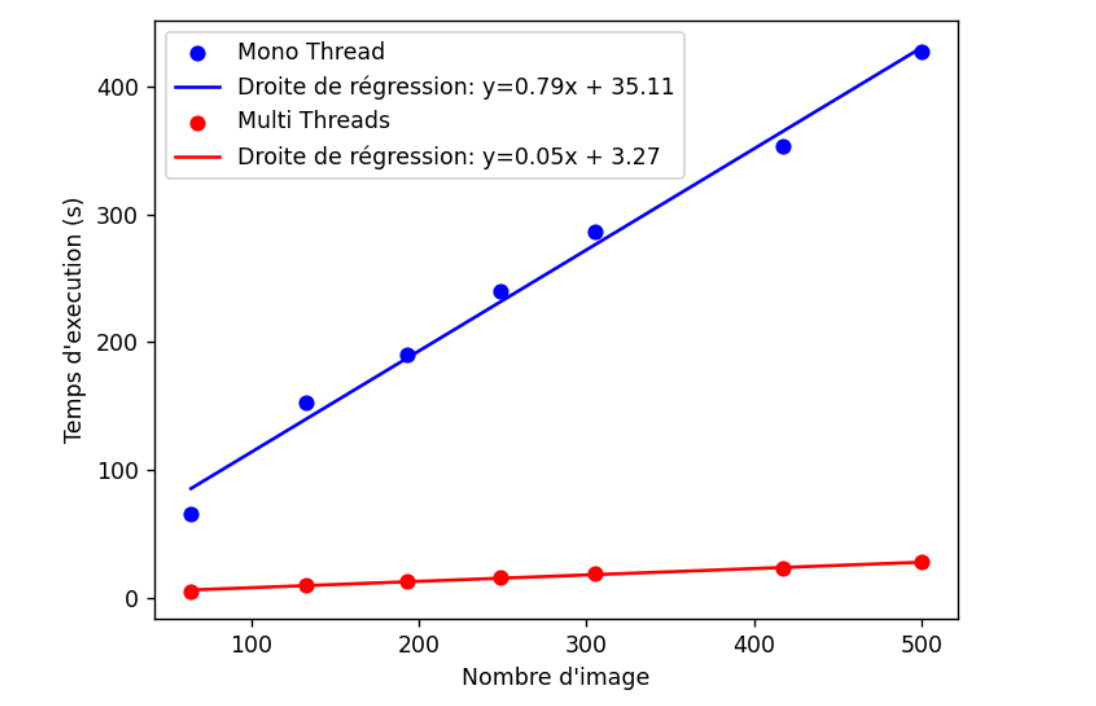
\includegraphics[width=0.8\textwidth]{assets/Capture d'écran process/general/multithread.png}
                \caption{Impact du multi-threading sur le processus MoCapIA}
                \label{fig:multithreading}
            \end{figure}
            Alors que le temps d'exécution en seconde augmente proportionnellement avec le nombre d'images à traiter dans une approche mono-thread, l'approche multithread maintient un temps d'exécution quasi constant. 

            Enfin l'équipe a jugé nécessaire de développer une interface graphique pour rendre le logiciel plus accessible et ergonomique. Pour ça un cahier des charges a été établi pour définir les fonctionnalités et l'apparence de l'interface. Il a donc instauré une structure de fichiers claire et intuitive pour chaque expérience, sujet et session. Les GoPro, utilisables avec différentes résolutions et fréquences d'images, sont maintenant configurables directement depuis l'interface. Le choix s'est porté sur une configuration de projet basé sur trois fichiers .JSON afin de stocker dans un premier les réglages du logiciel (raccourcis, fonctionnalités en option), dans un deuxième les informations relatives au statut du projet et dans un troisième les informations sur les caméras (résolution, fréquence d'images, angle de vue, paramètres intrinsèques, calibration extrinsèque). Graphiquement parlant, le logiciel construit se divisait en deux sections principales. La première section \textit{Acquisition} (figure \ref{fig:interface_colin1}) permet de gérer les expériences, les caméras et surtout de lancer les différentes étapes du processus :
            \begin{figure}[H]
                \centering
                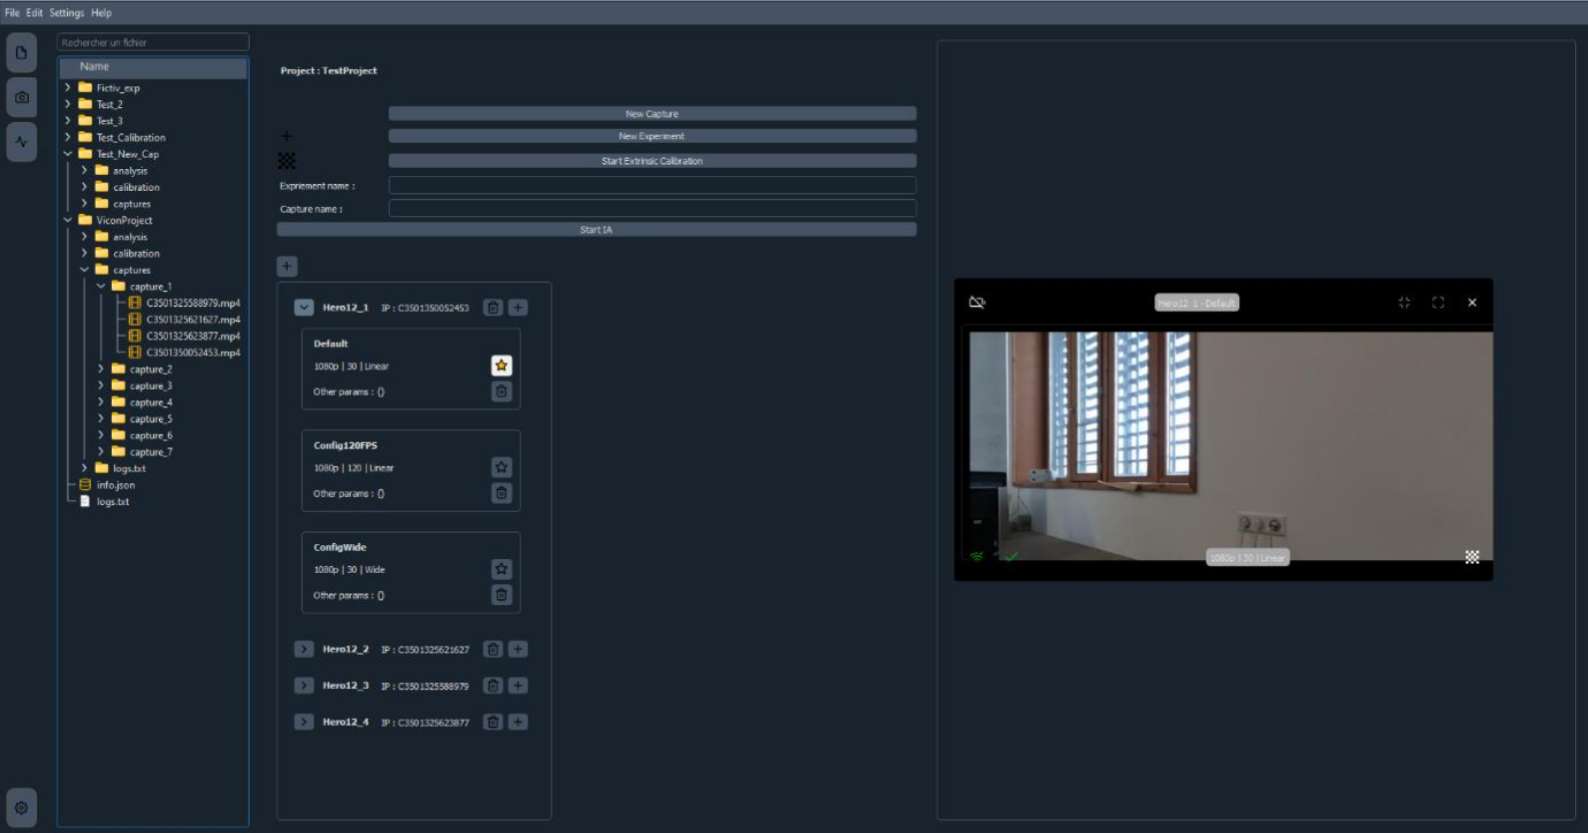
\includegraphics[width=0.8\textwidth]{assets/Capture d'écran process/general/interface_colin1.png}
                \caption{Section 1 de l'Interface graphique développée par le troisième stagiaire}
                \label{fig:interface_colin1}
            \end{figure}
            L'autre aspect important du cahier des charges consistait à permettre la visualisation du modèle 3D directement dans l'interface. C'est pourquoi dans une deuxième section \textit{Visualisation} (figure \ref{fig:interface_colin2}), l'utilisateur peut visualiser le modèle 3D sur le mouvement sélectionné. Il est possible en plus d'afficher les distances entre deux points du modèle ou l'angle entre 3 points pour permettre une analyse biomécanique rapide. C'est le premier grand pas vers une utilisation clinique ou sportive du système MoCapIA. 
            \begin{figure}[H]
                \centering
                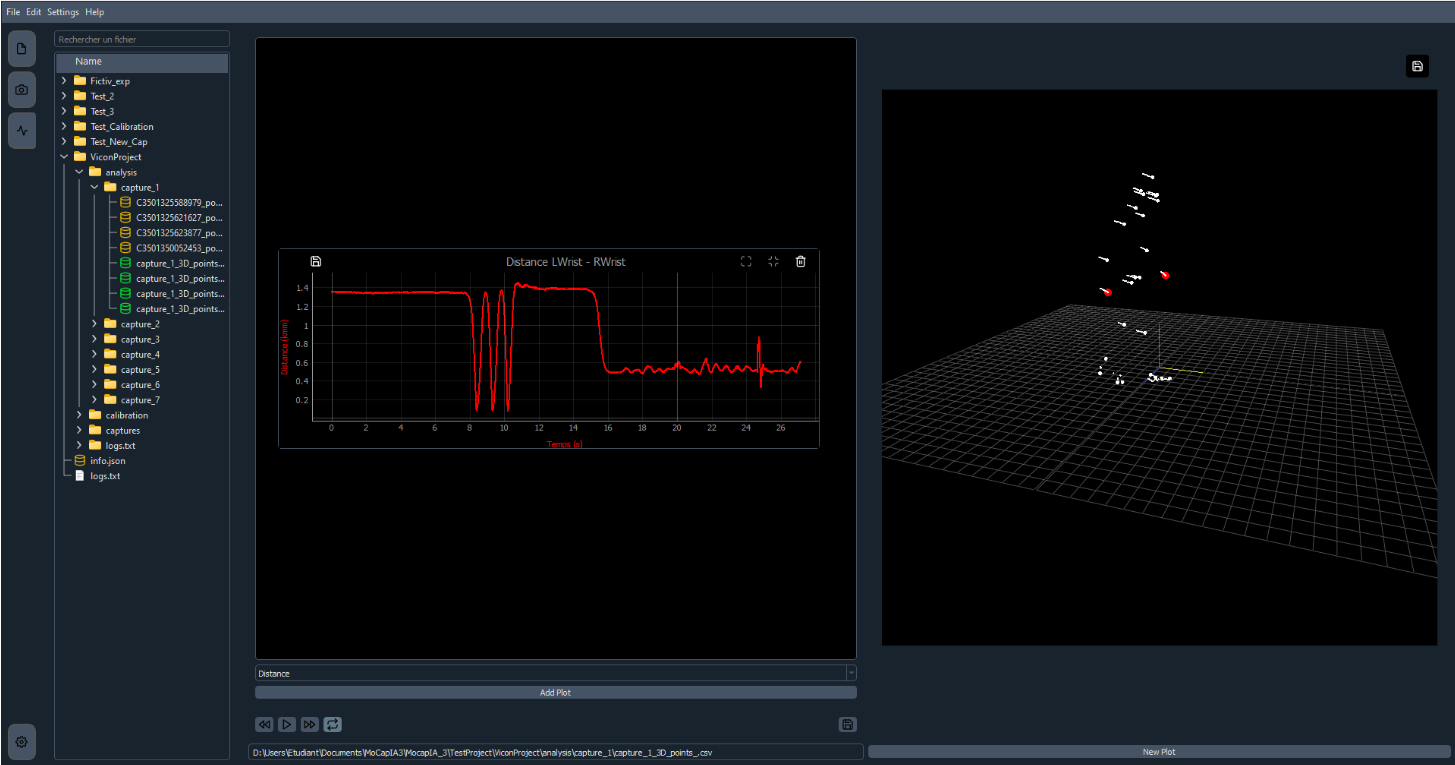
\includegraphics[width=0.8\textwidth]{assets/Capture d'écran process/general/interface_colin2.png}
                \caption{Section 2 de l'Interface graphique}
                \label{fig:interface_colin2}
            \end{figure}
        
            \item \textbf{Stagiaire 4 :} Durant le semestre P25, le quatrième stagiaire a principalement travaillé sur l'optimisation du processus MoCapIA et l'amélioration de l'interface graphique. Un affichage en temps réel de la progression par l'intermédiaire de logs et de barre de progression a été développé ce qui permet de suivre l'avancement de chacune des étapes. 
            Une méthode \textit{binning} a été implémentée dans la triangulation. Cette méthode permet de regrouper les différents points 3D candidats générés par chaque paire de caméras dans des intervalles. Le point final est obtenu en faisant la moyenne des points dans \textbf{l'intervalle ayant le plus de candidats}. Cet ajout rend la triangulation plus robuste face aux erreurs importantes. 
        \end{itemize}

\section{Le planning}

    La mise en place des tâches s'est faite lors de réunion hebdomadaire avec le tuteur de stage et parfois l'ensemble de l'équipe. Pour autant, les échanges étaient beaucoup plus fréquents, donc plusieurs ajustements ont été réalisés en fonction des imprévus et des découvertes faites par le tuteur de stage ou nous les stagiaires. Le planning général est présenté ci-dessous dans le tableau \ref{tab:planning}.

    \begin{table}[h!]
        \centering
        \renewcommand{\arraystretch}{1.5}
        \begin{tabularx}{\textwidth}{|c|c|X|} 
            \hline
            \textbf{Période} & \textbf{Phase} & \textbf{Description} \\
            \hline
            Semaine 1 & Prise en main & Réalisation du processus en entier sur l'ordinateur du précédent stagiaire (Ui, capture du mouvement, calibration, gestion des GoPro) \\
            \hline
            Semaine 2 & Installation & Étant donné que nous sommes deux, il a fallu installer le logiciel sur un nouvel ordinateur pour qu'il puisse lancer le logiciel avec les bonnes versions \\
            \hline
            Semaine 3 & Recherches Bibliographiques & Recherche sur les différentes étapes du processus MoCapIA, compréhension des principes mathématiques et informatiques \\
            \hline
            Semaines 4 à 6 & Tests de calibration & Réalisation de plusieurs tests pour évaluer la qualité de la calibration en fonction de différents paramètres (type de damier, nombre d'images, position des caméras) \\
            \hline
            Semaines 7 à 9 & Recherche sur la triangulation & Étude des différentes méthodes de triangulation et test sur la triangulation globale \\
            \hline
            Semaine 10 & Test de l'estimation 2D & Réalisation de plusieurs tests pour évaluer la qualité de l'estimation 2D en comparaison avec le Vicon \\
            \hline
            Semaines 11 à 14 & Ajout de nouvelles fonctionnalités & Ajout des étapes de filtrage, d'augmentation de marqueur, et de cinématique inversée \\
            \hline
            Semaines 15 à 17 & SAM 3D & Recherche sur le modèle SAM 3D de Meta et réalisation de tests \\
            \hline
            Semaines 18 à 20 & Rapport & Rédaction du rapport de stage \\
            \hline
        \end{tabularx}
        \caption{Répartition des tâches durant le stage}
        \label{tab:planning}
    \end{table}


\section{Outils et Technologies}

    \subsection{Hardware (matériels)}

        \subsubsection{Configuration de l'ordinateur}
        \begin{itemize}
            \item Processeur (CPU) : Intel Core i9-14900K
            \item Mémoire vive (RAM) : 64 Go
            \item Carte graphique (GPU) : NVIDIA GeForce RTX 4090
        \end{itemize}
        Ces composants haut de gammes ont eu un réel impact sur la rapidité d'exécution du processus MoCapIA, notamment grâce à la carte graphique qui permet d'accélérer les calculs liés à l'Intelligence Artificielle.
        
        \subsubsection{Systèmes de caméras}

        \begin{table}[h!]
        \centering
        \renewcommand{\arraystretch}{1.5}
        \begin{tabularx}{\textwidth}{|c|c|X|} 
            \hline
             & \textbf{MoCapIA} & \textbf{Vicon (référence)}\\
            \hline
            Nombre de caméras & 4 caméras GoPro Hero 12 Black \ref{fig:gopro} & 37 caméras infrarouges MXT160, Bonita 3 et Vantage 5 \\
            \hline
            Résolution utilisée & 1080 pixels & 16 mégapixels\\
            \hline
            Images par seconde (ips) & 30 & 120 \\
            \hline
            synchronisation & < 10 microsecondes & < 1 milliseconde (horloge de phase) \\
            \hline
        \end{tabularx}
        \caption{Comparaison des différents systèmes de caméras}
        \label{tab:cameras}
    \end{table}

    \begin{figure}[H]
        \centering
        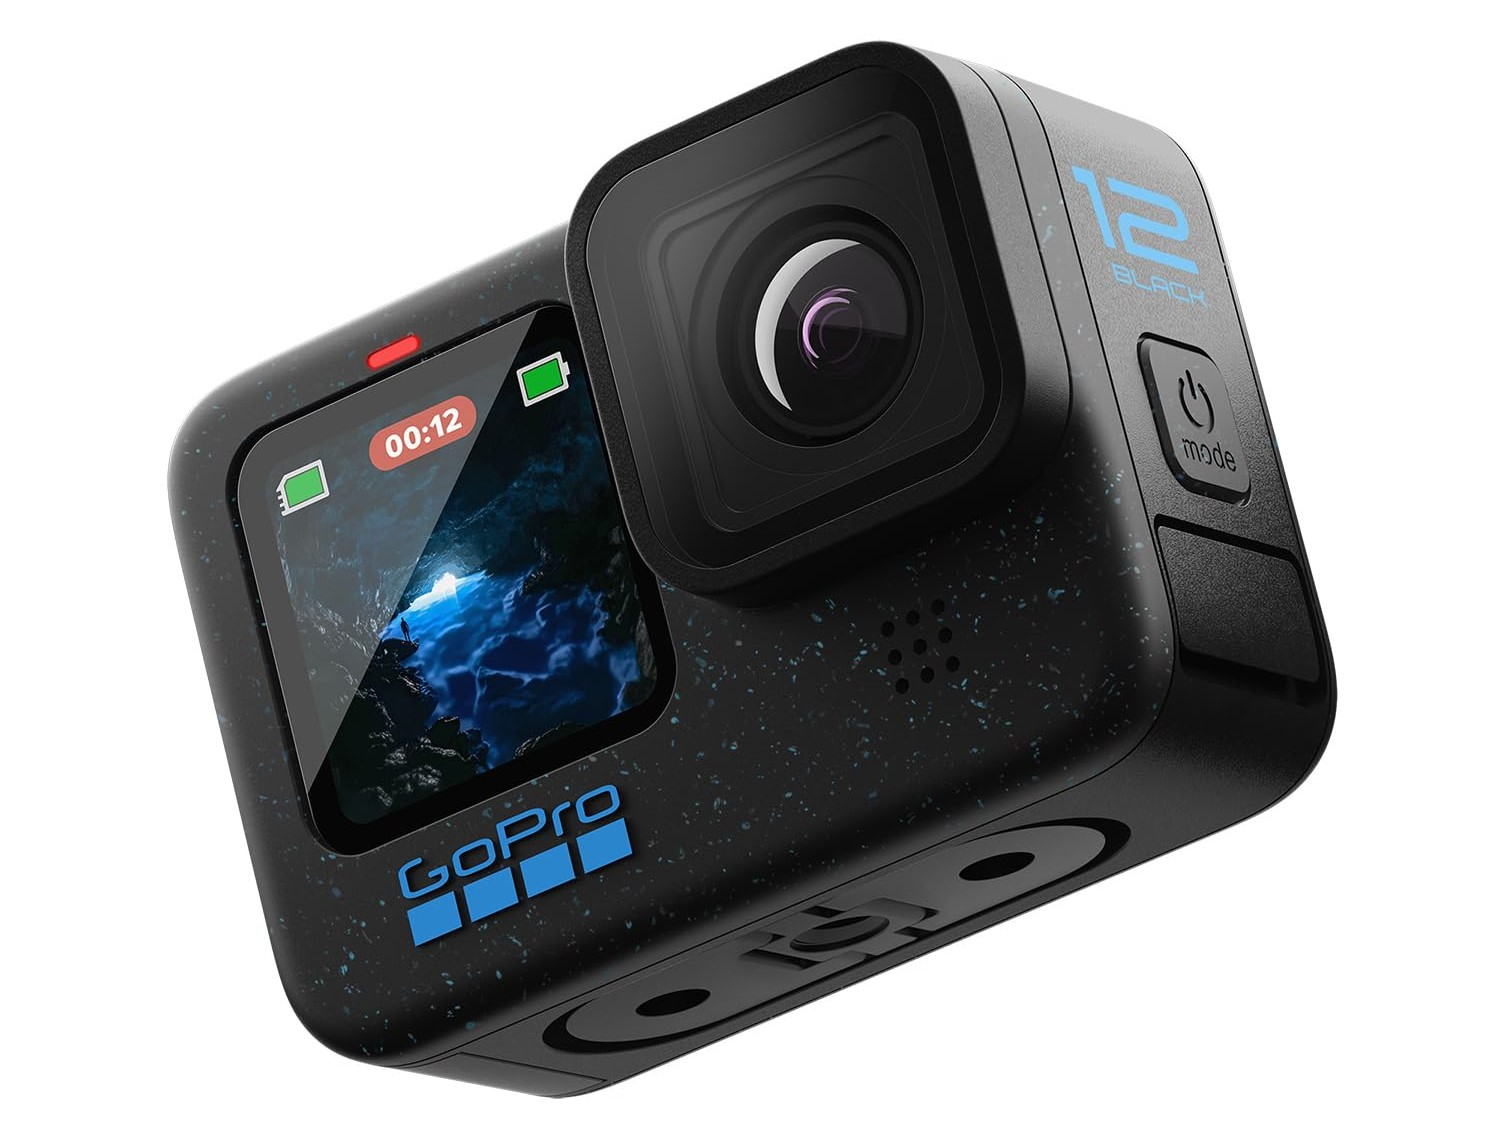
\includegraphics[width=0.65\linewidth]{assets/Capture d'écran process/general/gopro.jpg}
        \caption{Caméra GoPro Héro 12 Black}
        \label{fig:gopro}
    \end{figure}

        Grâce à la plateforme TSS, il a été possible d'accéder au système de référence Vicon/Nexus. C'est un système de motion capture avec marqueurs incluant :
        \begin{itemize}
            \item 18 caméras MXT160
            \item 12 caméras Bonita 3
            \item 7 caméras Vantage 5
            \item baguette de calibration à LED.

        \end{itemize}

        \subsection{Software}
            \subsubsection{Structure de fichiers}
            Pour organiser les données de chaque expérience, une structure de fichiers claire et intuitive a été mise en place :
            \begin{itemize}
                \item \textbf{fichier .pickle:} pour stocker les paramètres de calibration intrinsèques de chaque caméra
                \item \textbf{fichier .hdf5:} pour stocker l'ensemble des paramètres de calibration (intrinsèques et extrinsèques) de chaque caméra après calibration
                \item \textbf{fichier .json:} pour stocker les points 2D détectés par le modèle d'IA pour chaque caméra et les paramètres du projet
                \item \textbf{fichier .csv:} pour stocker les coordonnées 3D triangulées du modèle final
                \item \textbf{fichier .log:} pour stocker les logs générés durant chaque étape du processus MoCapIA
                \item \textbf{fichier .mp4:} pour stocker les vidéos capturées par chaque caméra durant l'expérience
                \item \textbf{fichier .trc:} pour stocker les données 3D - types de fichiers acceptés par OpenSim contrairement aux fichiers CSV
                \item \textbf{fichier .osim:} pour stocker le modèle osseux calculé par le package opensim
                \item \textbf{fichier .mot:} pour stocker les angles articulaires calculés par la \textit{cinématique inverse} d'OpenSim
                \item \textbf{fichier .xml:} pour stocker les paramètres de \textit{scaling} et de \textit{cinématique inverse} d'OpenSim
            \end{itemize}

            \subsubsection{Logiciel}
                \begin{itemize}
                    \item OpenSim 4.5 : pour l'analyse biomécanique du modèle 3D (scaling, cinématique inverse)
                    \item Visual Studio Code : pour le développement en Python et l'écriture du rapport
                    \item Anaconda : pour la gestion des environnements Python et des dépendances
                    \item Git et GitLab UTC : pour le versionnage du code source et la collaboration entre les stagiaires
                    \item GoPro Quik : application Android pour la gestion et la synchronisation des caméras GoPro
                    \item MATLAB : pour la majorité des tests et des analyses d'erreurs
                    \item Notion : pour la prise de notes et le suivi personnel du projet
                \end{itemize}

            \subsubsection{Langage de Programmation}
                \begin{itemize}
                    \item Python 3.8.19 : pour le développement du logiciel MoCapIA (version utilisée par les précédents stagiaires)
                    \item Python 3.10.18 : pour le développement de la partie OpenSim (le changement d'environnement est nécessaire pour la compatibilité avec le package OpenSim mais cela reste automatique)
                    \item Python 3.11.14 : pour le développement de SAM 3D
                    \item Langage MATLAB R2023b
                    \item Langage Latex : pour la rédaction du rapport de stage
                \end{itemize}

        \subsection{FabLab}
        De plus, par la proximité avec le FabLab, il a été possible de créer des pièces sur mesures pour les besoins et les différentes expériences menées durant le projet. Des damiers de calibration de différentes tailles ont été imprimés pour un test sur leur impact sur la qualité de la calibration. Un robot articulé UR3 a été utilisé pour simuler des mouvements précis et répétables lors des tests de calibration.
        \begin{figure}[H]
            \centering
            \begin{subfigure}[b]{0.48\textwidth}
                \centering
                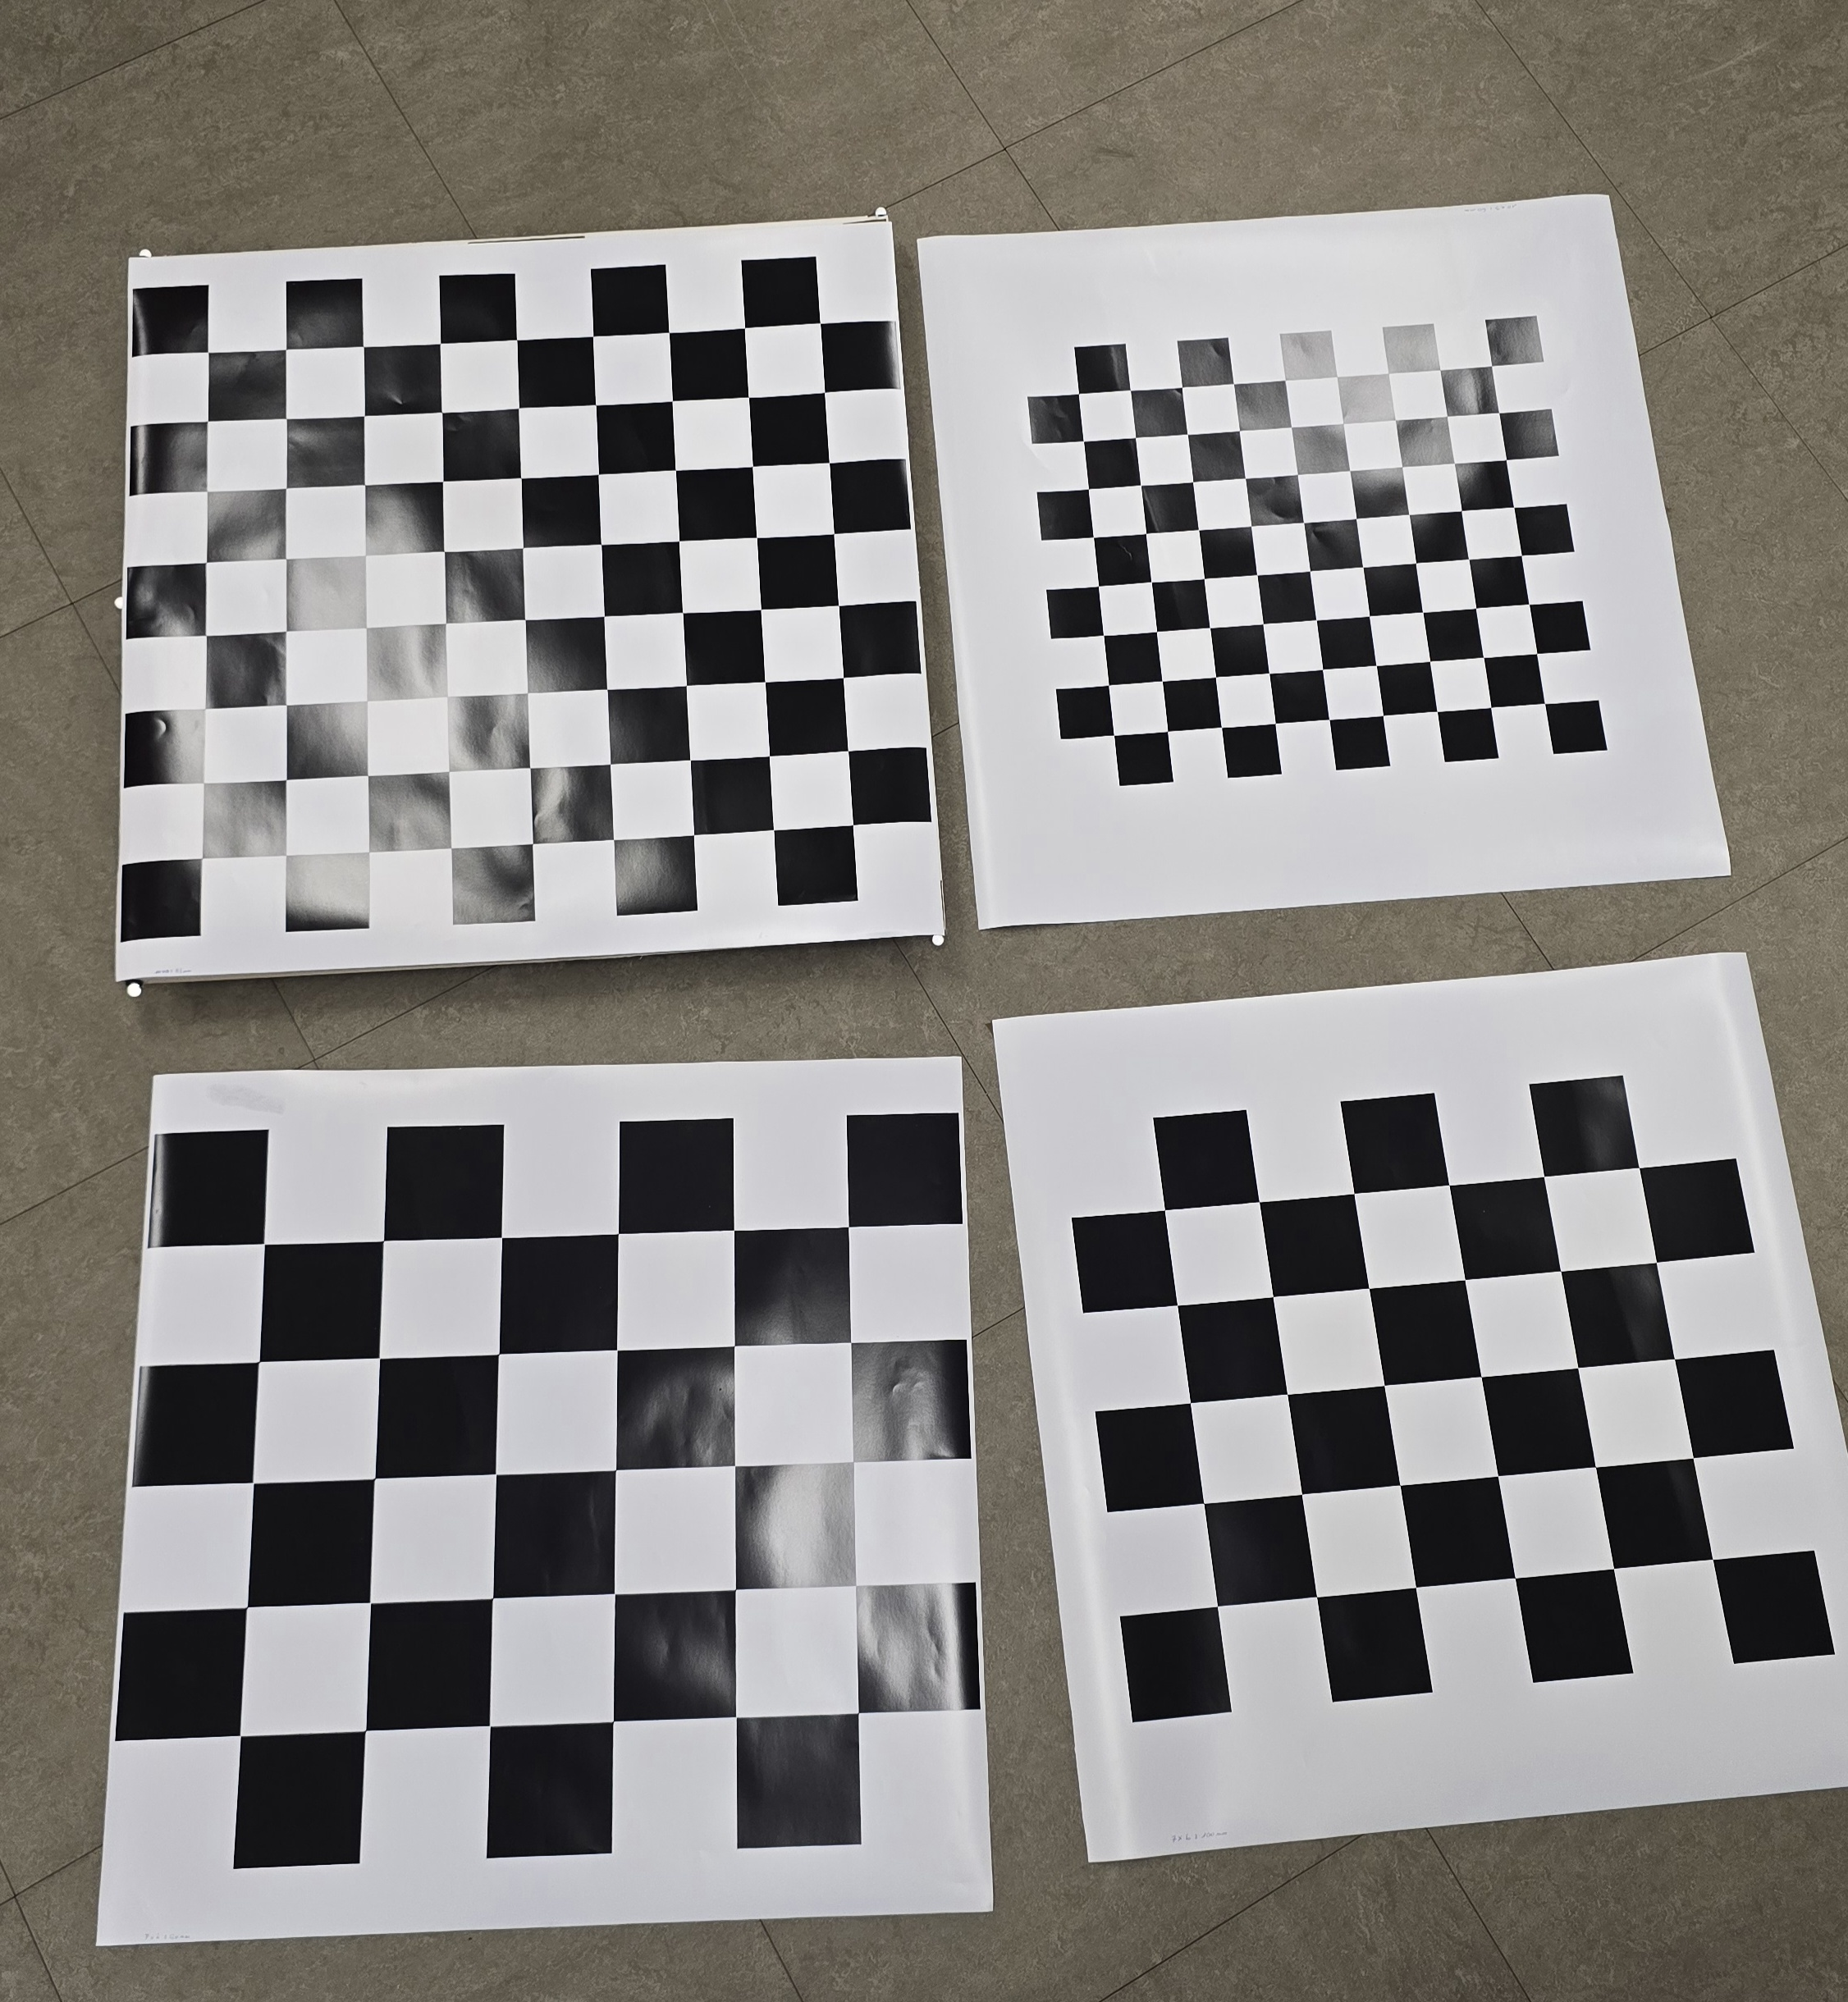
\includegraphics[width=\linewidth]{assets/Capture d'écran process/Test_Damiers/damiers_imprimés.jpg}
                \caption{Damiers de calibration imprimés}
                \label{fig:damiers_fablab}
            \end{subfigure}
            \hfill
            \begin{subfigure}[b]{0.48\textwidth}
                \centering
                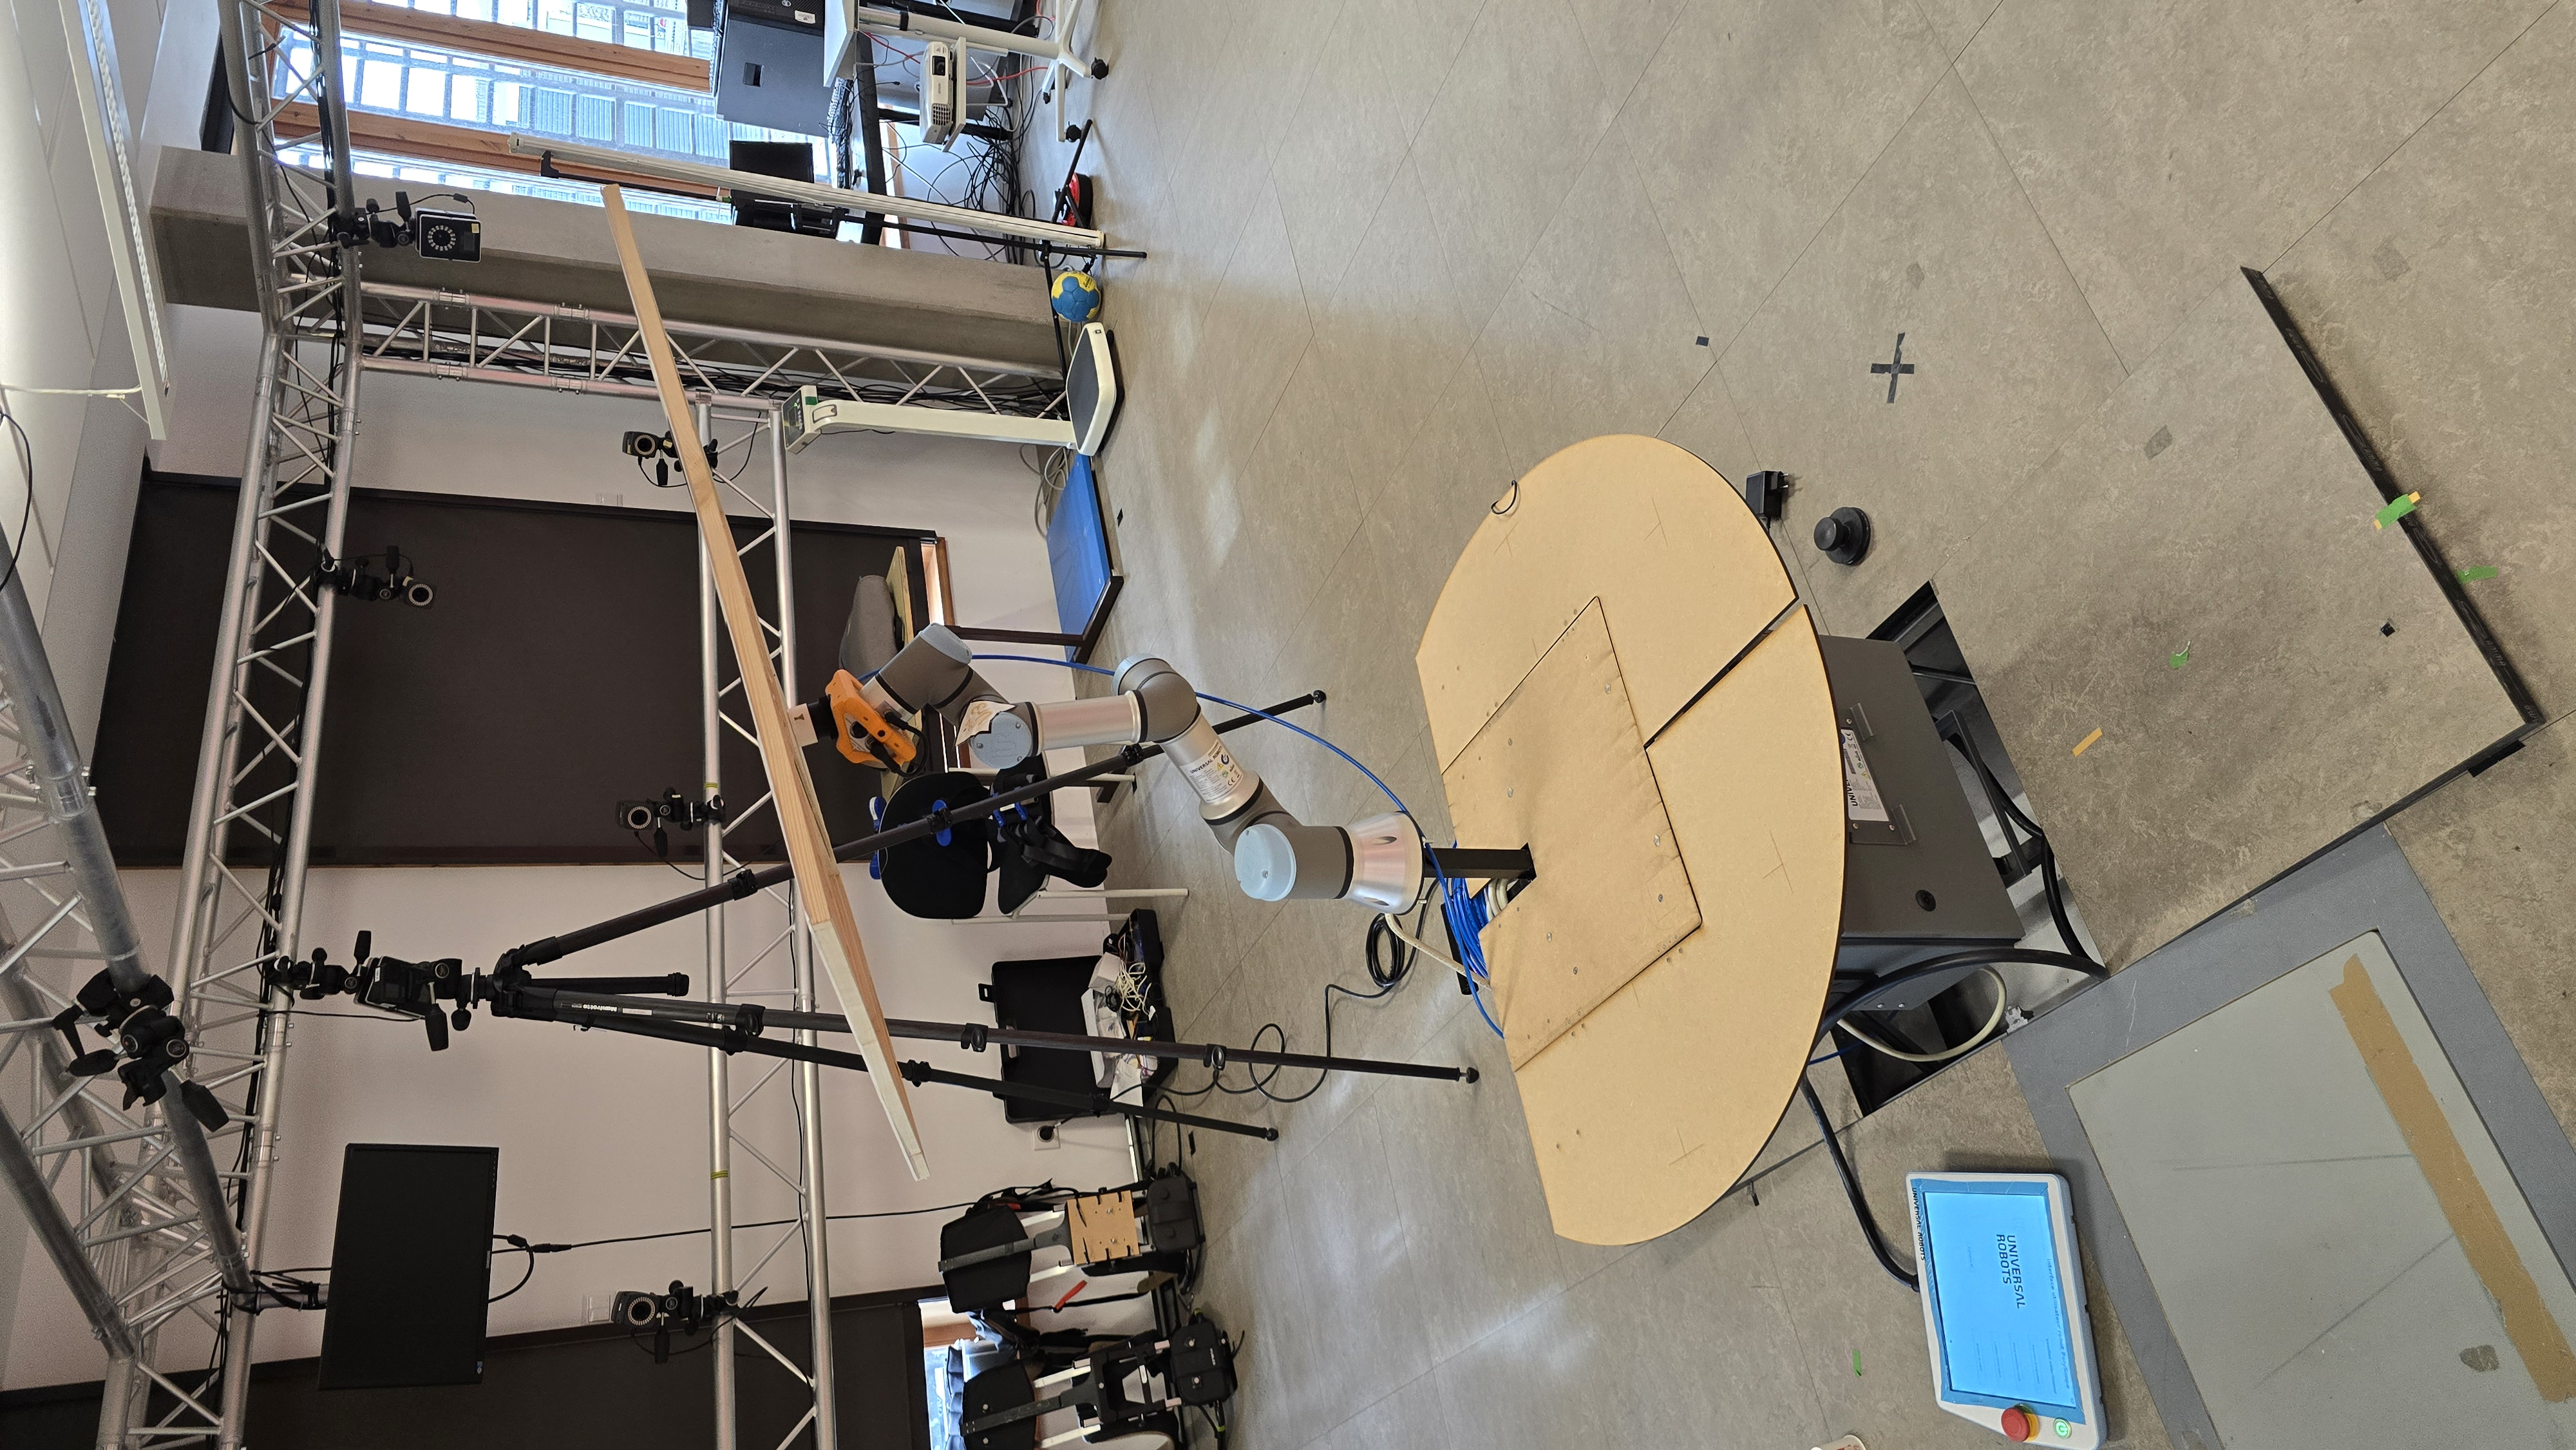
\includegraphics[width=\linewidth, angle=-90]{assets/Capture d'écran process/Test_Damiers/robot.jpg}
                \caption{Robot articulé de test}
                \label{fig:robot_articulé}
            \end{subfigure}
            \caption{Matériel utilisé pour le test sur l'impact des damiers sur la calibration}
            \label{fig:materiel_tests}
        \end{figure}
    \chapter{Mes réalisations}
\label{Réalisations}

    Nous allons maintenant explorer mes contributions concrètes au projet MoCapIA.
    Même si le projet est assez performant, simple d'utilisation et rapide, les erreurs totales observées à la fin du processus restent trop importantes pour une analyse biomécanique sérieuse et une utilisation dans le domaine sportif. En traçant la distance entre deux points (ex : hanche droite et genou droit) au cours d'un mouvement, la valeur fluctue énormément et des valeurs aberrantes sont observées. Voici un graphe représentant la distance entre les deux points cités précédemment au cours d'un mouvement de squat : on observe une variation de $\pm 40mm$ pour une distance qui devrait théoriquement rester constante. 
    \begin{figure}[h]
        \centering
        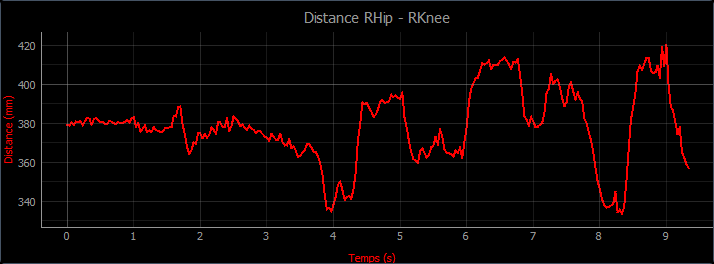
\includegraphics[width=0.8\textwidth]{assets/Capture d'écran process/resultFinDeStage/DEBUTSTAGEDistance_RHip_-_RKnee_.png}
        \caption{Distance entre hanche droite et genou droit – début de stage}
        \label{fig:distance_hip_knee_debut_stage} 
    \end{figure}
    Ce sont des erreurs trop importantes et la suite du chapitre va se focaliser sur les mesures prises pour améliorer la précision et la stabilité du système.

    Mais avant tout, il est d'abord nécessaire de comprendre d'où viennent les erreurs. Comme expliqué préalablement, MoCapIA se décompose en 3 étapes principales : la calibration, l'estimation 2D et la triangulation. Chacune de ces étapes peut engendrer des erreurs. Il est donc primordial d'analyser chacune de ces étapes pour comprendre où se situent les principales sources d'erreurs. Voici le plan que nous allons suivre dans ce chapitre :
    \begin{itemize}
        \item \textbf{TEST 0 - Analyse de l'effet du damier sur la calibration :} dans ce test, l'objectif est d'analyser l'impact du damier en utilisant différentes configurations (taille des carreaux, nombre de carreaux).
        \item \textbf{TEST 1 - Analyse de l'homogénéisation de la calibration :} on cherche cette fois à mesurer la précision de la calibration à différents endroits de la zone de capture en isolant les erreurs liées à l'estimation 2D (IA).
        \item \textbf{TEST 2 - Analyse de l'estimation 2D par l'IA :} ici, l'objectif est de mesurer les erreurs liées à l'estimation 2D en utilisant le système Vicon comme référence.
    \end{itemize}   
    Enfin, nous essayerons d'apporter différentes solutions pour améliorer la précision globale du système.
    
    \begin{figure}[H]
        \centering
        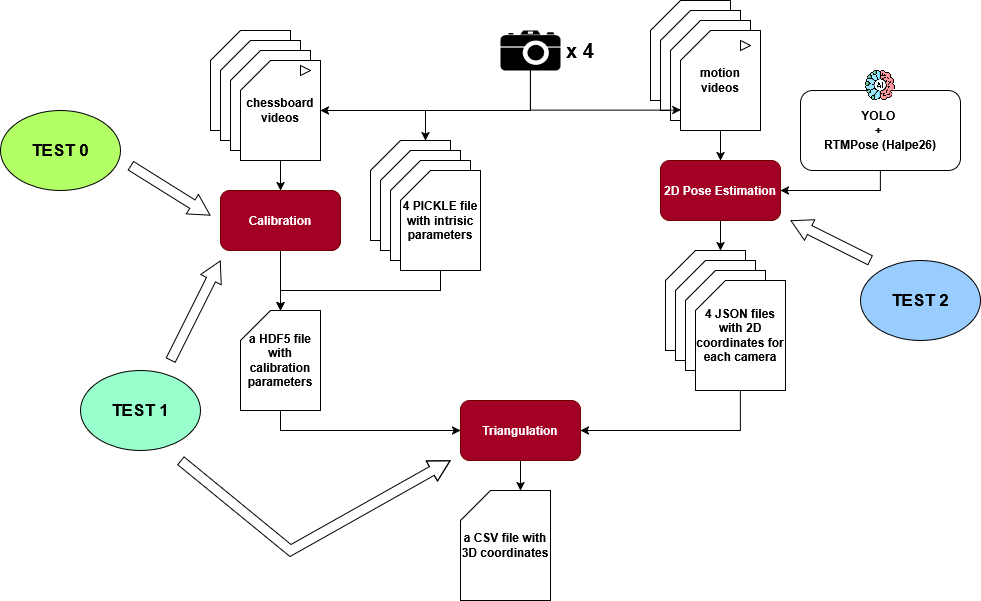
\includegraphics[width=\textwidth]{assets/Capture d'écran process/general/synthèseMOCAPIA_tests.drawio.png}
        \caption{Schéma récapitulatif des tests effectués}
        \label{fig:synthese_tests_mocapia}
    \end{figure}

\section{Analyse des erreurs liées à la calibration}

    La calibration et la triangulation sont les étapes mathématiques de base, mais essentielles pour notre logiciel ; il était important d'en connaître la précision et donc mesurer les erreurs qui sont liées à ces étapes. Pour ça il a fallu les isoler des erreurs liées à l'estimation 2D (traitées juste après).
    Pour l'étude suivante, on part de l'hypothèse suivante : dans un scénario théorique idéal (calibration et détection sans erreurs), la méthode DLT est exacte. Elle ne génère aucun biais ni erreur résiduelle intrinsèque (0 mm). L'erreur de reconstruction observée en pratique provient exclusivement de la propagation des incertitudes d'entrée (bruit de détection 2D et imprécisions de calibration) et non de la formulation mathématique de la DLT elle-même \cite{Triangulation}. Il est donc possible d'isoler les erreurs liées à la calibration même si on est capable d'observer les erreurs seulement après la triangulation.

    \subsection{TEST 0 - Analyse de l'effet du damier sur la calibration}

        Cette première analyse vise à mesurer l'impact du damier utilisé pour la calibration. Deux paramètres sont à étudier : la taille des carreaux qui composent le damier ainsi que leur nombre. Pour ça, 4 damiers de tailles différentes ont été fabriqués avec l'aide du FabLab (voir figure \ref{fig:damiers_fablab}) :
        \begin{itemize}
            \item Damier A : 7x6 carreaux de 120 mm
            \item Damier B : 7x6 carreaux de 100 mm
            \item Damier C : 10x9 carreaux de 85 mm
            \item Damier D : 10x9 carreaux de 60 mm.
        \end{itemize}

        Mais pour pouvoir comparer la calibration, il faut pouvoir exécuter le même mouvement à chaque fois. Pour ça, un bras articulé UR3 (\ref{fig:robot_articulé}) capable de reproduire exactement le même mouvement à chaque itération a été utilisé. En fixant les différents damiers sur le robot, il est maintenant possible de comparer la calibration obtenue avec chaque damier. 
        \begin{figure}[h]
            \centering % Pour centrer l'image
            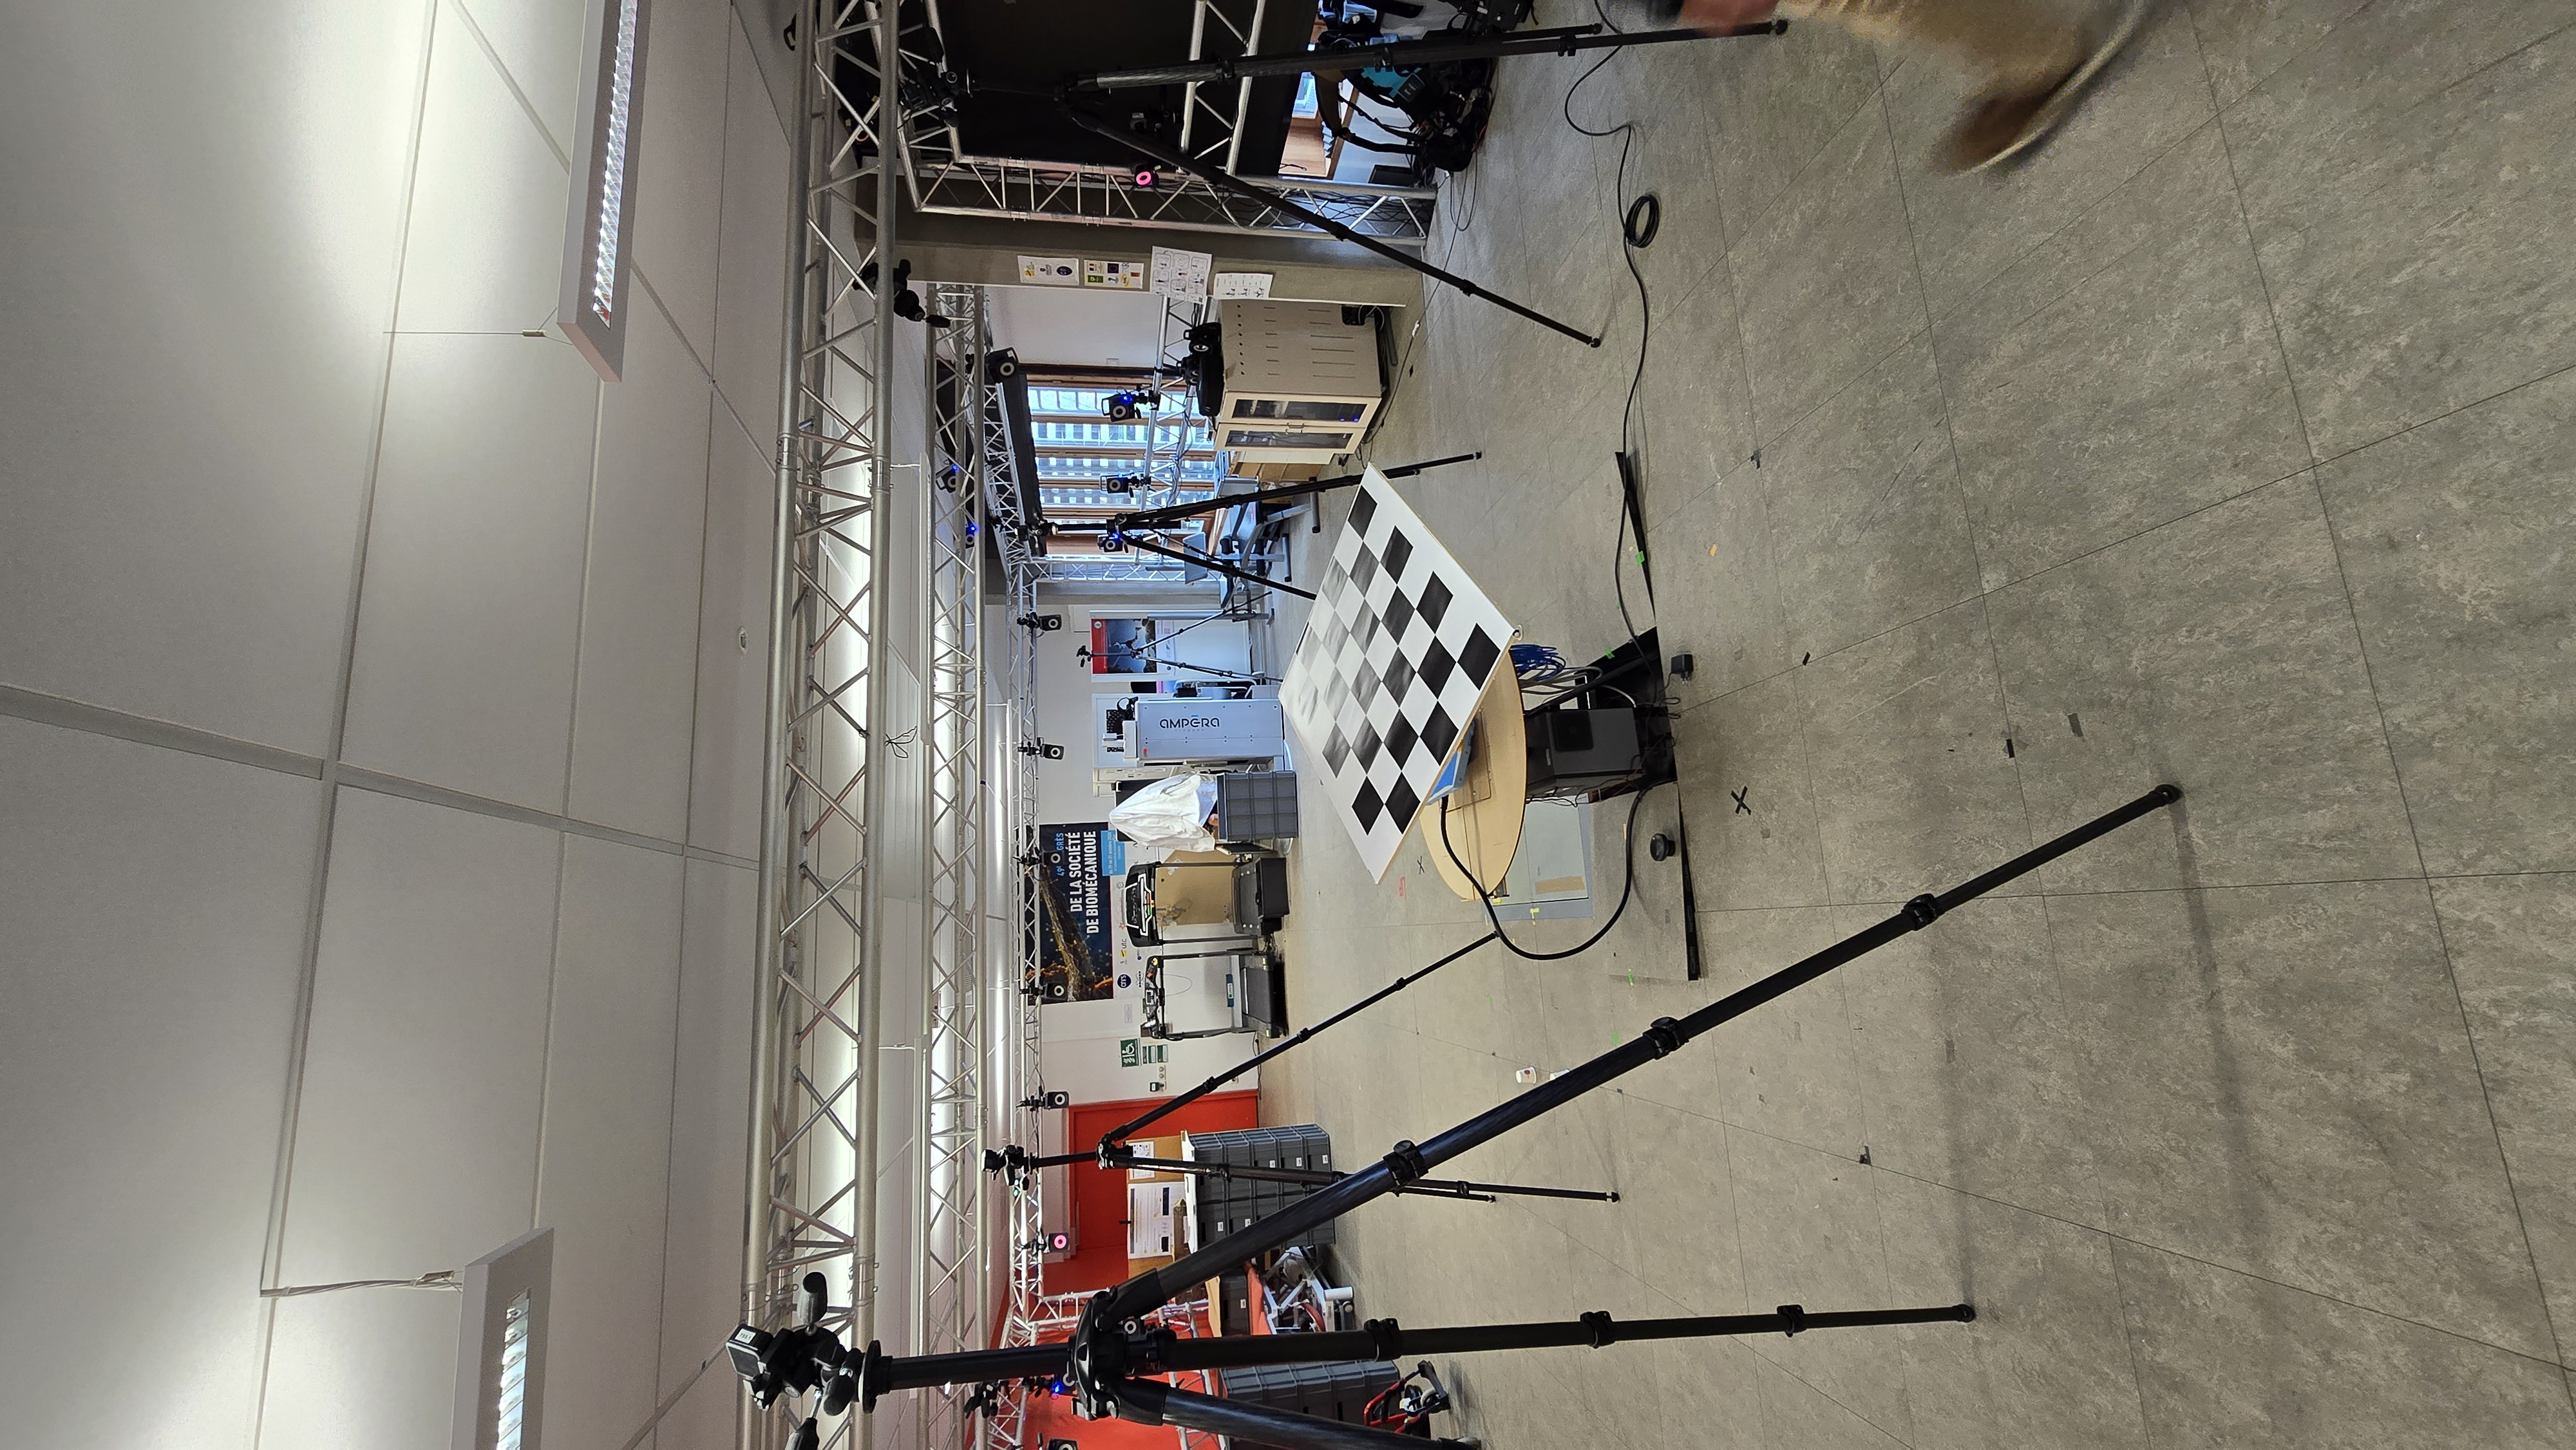
\includegraphics[width=0.8\textwidth, angle=-90]{assets/Capture d'écran process/Test_Damiers/scene_robot.jpg}
            \caption{Scène de calibration avec le bras articulé}
            \label{fig:scène_robot}
        \end{figure}

        Les résultats ci-dessous ont été obtenus pour un mouvement de rotation du bras de 360 degrés. En utilisant la table ANOVA (Analyse de la Variance), on est capable de répondre à la question : \textit{"Est-ce que le fait de changer de damier change réellement la mesure, ou est-ce juste du hasard ?"}. Sur la table ANOVA, on observe que la valeur \textit{p value} est proche de zéro ($7.25671e^{-286}$) sur un jeu de donnée de $1389$ points par damier. Cette valeur signifie que le choix du damier à un impact significatif sur la précision et la qualité de la calibration. À l'aide de la fonction MATLAB \texttt{multcompare()} appliqué à la mesure du Bras gauche (segment ElbowL - ShoudlerL), on est capable de savoir quels damiers sont statistiquement différents les uns des autres en les séparant en différents groupes. Un groupe s'impose comme étant statistiquement proche, celui du damier 7x6 100 mm et 10x9 60 mm. La moyenne de ce groupe $\mu \approx 266 mm$ est validé par le fait qu'avec deux damiers de géométrie différente, les résultats sont proches. Les damiers 7x6 120 mm et 10x9 85 mm semblent sur-estimé la longueur du membre. En effet, la distance du bras du sujet étant de $d_bras = 270 mm$, les résultats de ces deux damiers sont considérés par le calcul ANOVA comme trop éloigné statistiquement pour que cet écart soit uniquement dû au bruit.
        \begin{figure}[H]
            \centering
            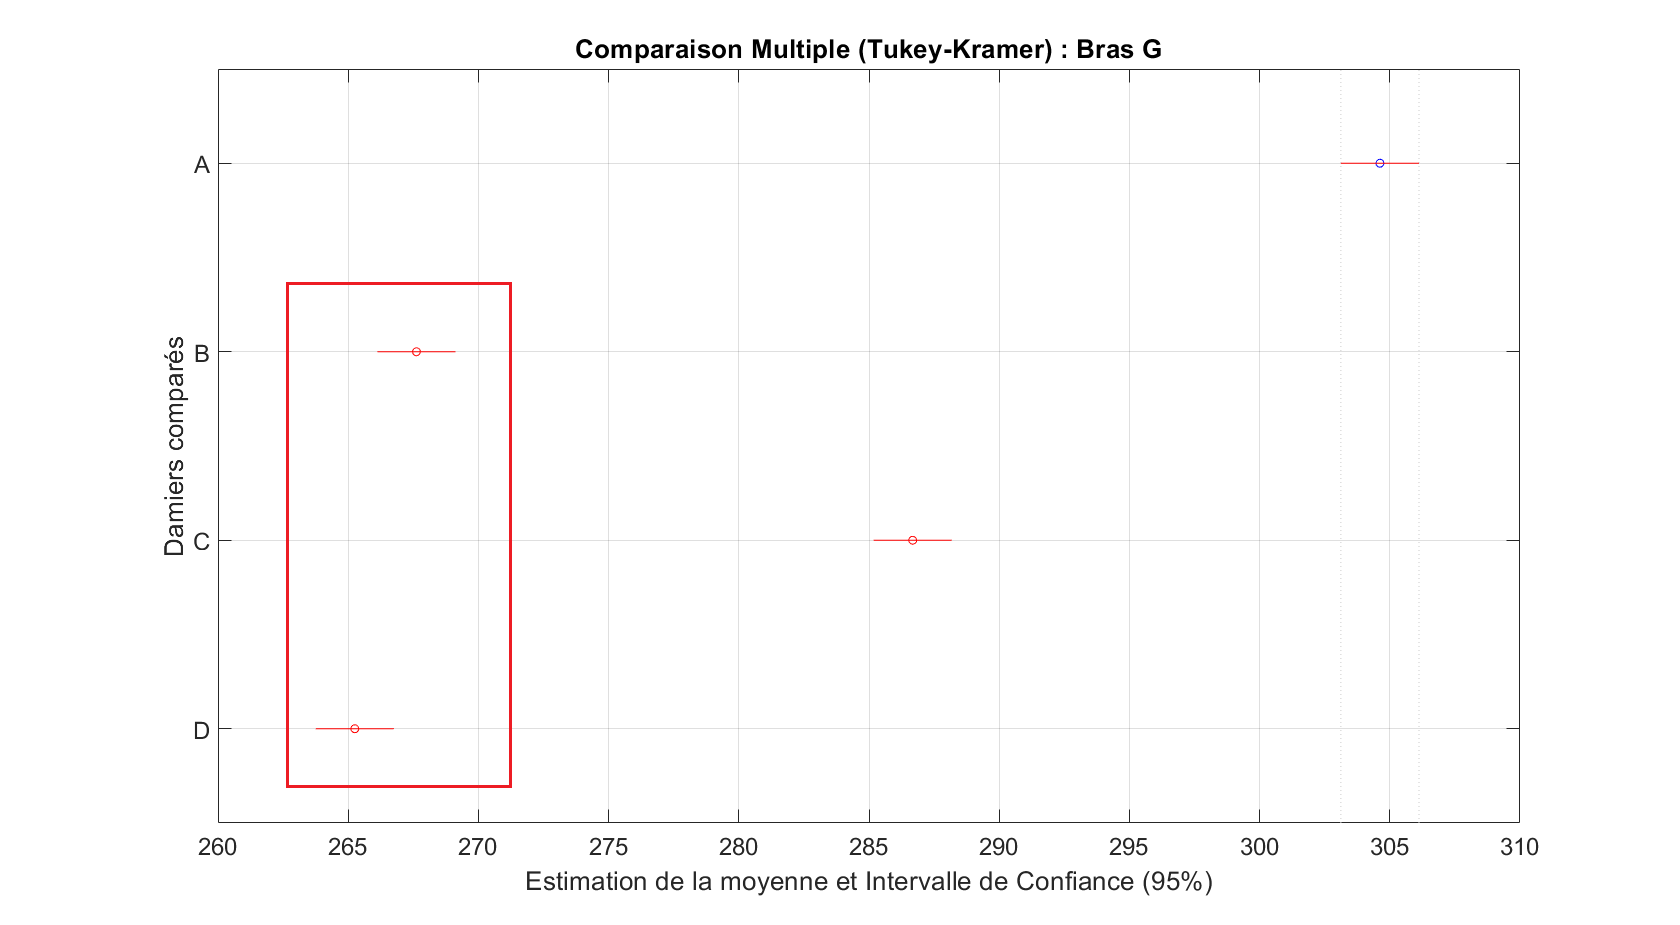
\includegraphics[width=\textwidth]{assets/Capture d'écran process/Test_Damiers/result_brasG.png}
            \caption{Graphique multcompare MATLAB des damiers}
            \label{fig:multcompare_damiers}
        \end{figure}

        Il a été décidé de compléter cette étude en observant la stabilité des résultats. Pour ça, une analyse \textit{boxplots} permet de conclure que la stabilité est bien plus forte avec le damier 10x9 60 mm et le damier 7x6 100 mm en plus d'être proche statistiquement parlant (\ref{boxplot_damiers}). Au contraire les damiers 7x6 120 mm et 10x9 85 mm présentent des quartiles plus écartés.
        \begin{figure}[H]
            \centering
            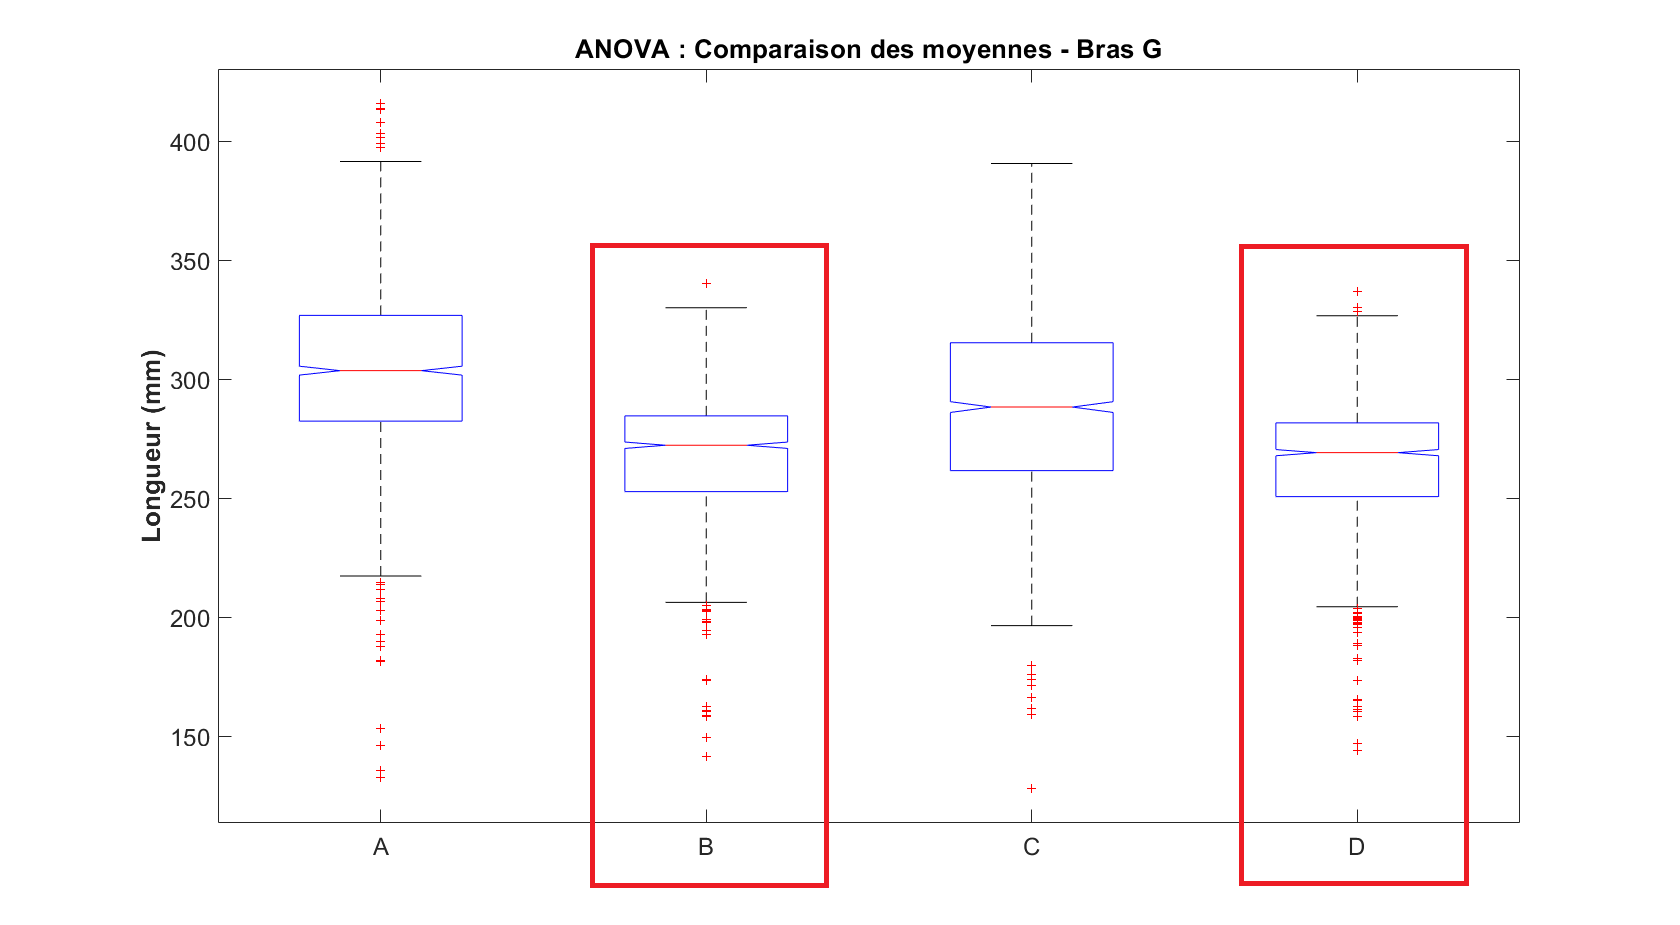
\includegraphics[width=\textwidth]{assets/Capture d'écran process/Test_Damiers/anova_boxplots_brasG.png}
            \caption{Boxplots sur la distance ElbowL - ShoulderL pour chaque damier}
            \label{boxplot_damiers}
        \end{figure}
        
        En conclusion, on remarque deux choses :
        \begin{itemize}
            \item Le nombre de carreaux n'a pas directement d'impact sur la précision de la calibration. En exemple, le damier 10x9 85 mm n'obtient pas de meilleurs résultats que le damier 7x6 100 mm ou 120 mm.
            \item La taille des carreaux n'a pas non plus un impact sur la calibration, car le damier 7x6 120 mm ne fait pas mieux que le damier 7x6 100 mm et le damier 10x9 85 mm ne fait pas mieux que le damier 10x9 60 mm.
            \item C'est plutôt la taille globale du damier qui a un impact sur la calibration. En effet, le damier 7x6 100 mm a une aire $A_1 \approx 0.42 m^2$ et le damier 10x9 60 mm a une aire $A_2 \approx 0.32 m^2$. Ces deux damiers sont ceux qui offrent les meilleurs résultats. À l'inverse, le damier 7x6 120 mm ($A_3 \approx 0.60 m^2$) et le damier 10x9 85 mm ($A_4 \approx 0.65 m^2$) sont ceux qui offrent les moins bons résultats. Ces résultats permettent d'émettre l'hypothèse que la \textbf{distorsion}, qui est plus importante sur les bords de l'image (appelé \textit{fisheye}), impacte fortement les résultats de la calibration \cite{CalibrationWeng}. En effet, en ayant un damier trop grand, les points caractéristiques situés sur les bords de l'image sont plus affectés par la distorsion, ce qui dégrade la calibration. Même si la distorsion est corrigée lors de la triangulation, elle ne l'est pas lors de la calibration. Pour utiliser un damier plus grand, il faudrait appliquer une correction de la distorsion lors de la calibration.
        \end{itemize}
        Pour la suite du projet, l'équipe a donc décidé d'utiliser le damier 7x6 100 mm qui offre un bon compromis entre précision et stabilité.

    \subsection{TEST 1 - Analyse de l'homogénéisation de la calibration}

        Maintenant que le damier est choisi, il est important de connaître la précision de la calibration. L'objectif ici est de mettre de côté les erreurs liées à l'estimation 2D pour se concentrer uniquement sur les erreurs liées à la calibration (nous avons vu dans l'introduction que la triangulation n'engendrait pas d'erreurs). Les coordonnées 2D utilisées seront obtenues à l'aide d'un clic-souris, précis au pixel (soit une précision) près grâce au zoom. Pour ça, une baguette de calibration a été utilisée contenant 3 points caractéristiques espacés de distances connues :
        \begin{itemize}
            \item Point 1 - Point 2 : 250 mm
            \item Point 2 - Point 3 : 243 mm
            \item Point 3 - Point 1 : 290 mm
        \end{itemize}
        La scène de test est représentée sur la figure \ref{fig:scène_verif_calib} ci-dessous. 
        \begin{figure}[H]
            \centering
            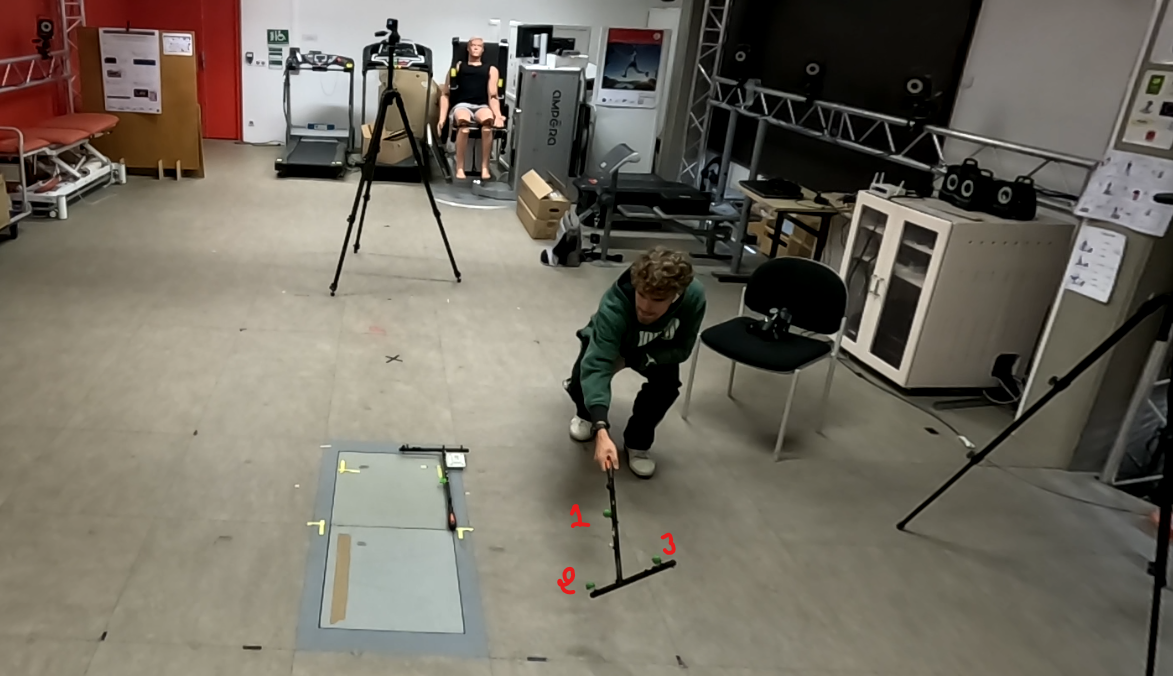
\includegraphics[width=0.8\textwidth]{assets/Capture d'écran process/Précision_CalibTriangulation/image.png}
            \caption{scène de vérification de points 3D}
            \label{fig:scène_verif_calib} % Une étiquette pour y faire référence
        \end{figure}
        \FloatBarrier
        Après avoir cliqué sur les 3 points caractéristiques à travers les 4 points de vue, les points triangulés (3D) sont comparés aux distances théoriques.
        Les erreurs sont représentées sur la figure \ref{fig:plot_calib_triang} qui représente la scène dans l'espace avec les caméras ainsi que les points caractéristiques de la baguette à plusieurs endroits dans la scène.
        \begin{figure}[H]
            \centering
            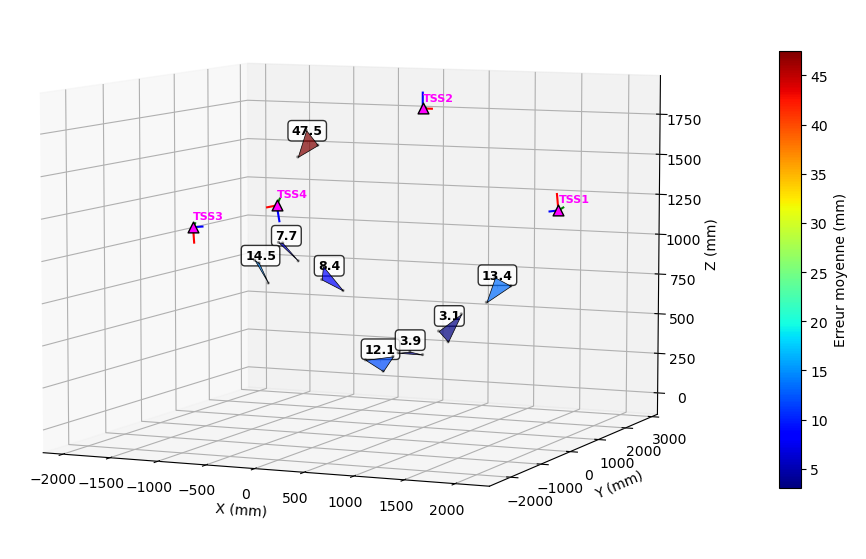
\includegraphics[width=0.8\textwidth]{assets/Capture d'écran process/Précision_CalibTriangulation/Figure_Calib.png}
            \caption{Résultat des erreurs de calibration après triangulation des 3 points caractéristiques}
            \label{fig:plot_calib_triang} % Une étiquette pour y faire référence
        \end{figure}
        
        La médiane des valeurs est de $8.4mm$. Cela représente une erreur relative de seulement $3.36\%$ pour une distance théorique de $250mm$. Étant donné que les erreurs totales observées précédemment étaient de l'ordre de la dizaine de centimètres, les résultats sont satisfaisants. 
        Cependant, certaines valeurs aberrantes ont été observées ($\approx 47.5mm$). Elles se situent proche des bords de la zone de capture. Cela indique donc que la précision de la calibration n'est pas totalement \textbf{homogène} sur l'ensemble de la zone commune (zone de capture). C'est donc un détail à prendre en compte lors du positionnement des caméras, mais aussi lors du mouvement du sujet.
        
        Finalement, pour un mouvement situé au centre de la zone de capture, \textbf{la calibration et la triangulation n'engendrent que très peu d'erreurs} sur le processus global. Une étude sur une autre méthode de triangulation (globale au lieu de locale) a été réalisée, mais n'a pas été concluante. Les résultats obtenus sont présentés en Annexe \ref{AnnexTriangu}.


\section{TEST 2 - Analyse de l'estimation 2D par l'IA}
\label{estimation2D}
    Pour rappel, nous utilisons deux modèles d'intelligence artificielle pour l'estimation 2D des points caractéristiques du corps humain : \textbf{YOLO} et \textbf{RTMPose}.
    En introduction, il avait été observé que des erreurs d'une dizaine de centimètres sur les longueurs des membres. De plus, la conclusion précédente permet d'affirmer que la majorité des erreurs proviennent de l'estimation 2D. Pour confirmer cette analyse, il faut calculer la précision et les erreurs liées à cette partie du processus. Pour ça on dispose d'un des systèmes les plus performants et précis qui existe : le Vicon. Précis à quelques millimètres près, il sera utilisé comme référence. Pour valider le résultat, il faut donc capturer les points caractéristiques du corps humain à la fois avec le Vicon, à la fois avec le MoCapIA et il va falloir comparer la distance entre chaque point 3D.
    Ce test a été réalisé en collaboration avec des étudiants en TX (Juliette Lafont et Dorian Biot). Sur la figure \ref{fig:yolo_rtmpose_vicon}, on peut voir la détection des points en 2D par YOLO (la boîte) et RTMPose (le squelette à 26 points) et éventuellement distinguer les marqueurs Vicon (les points lumineux blanc).

    \begin{figure}[H]
        \centering
        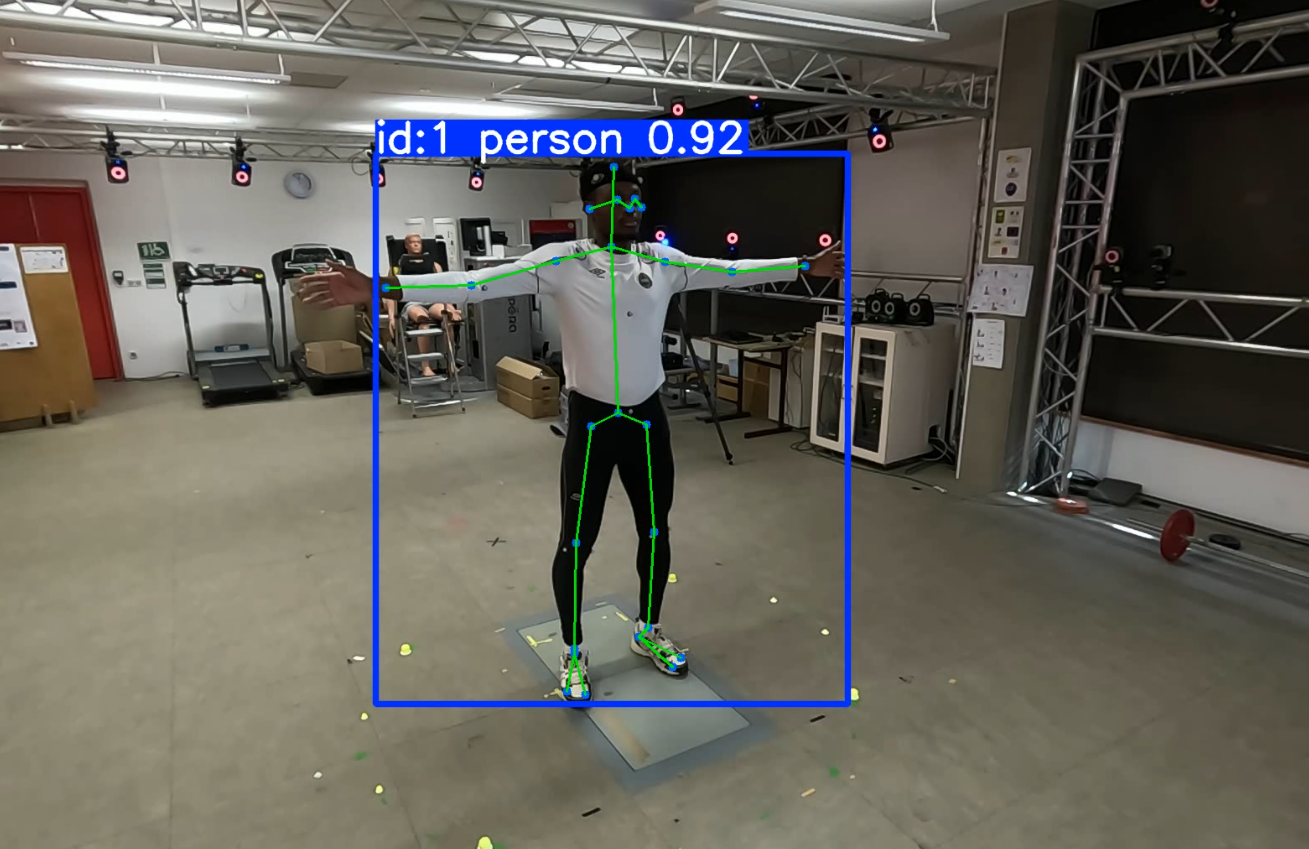
\includegraphics[width=\textwidth]{assets/Capture d'écran process/TX_ViconVSMocapIA/yolo_rtmpose.png}
        \caption{Marqueurs virtuels de MoCapIA et marqueurs physiques du Vicon}
        \label{fig:yolo_rtmpose_vicon}
    \end{figure}
    
    L'objectif de ce test est de comparer les deux systèmes de capture de mouvement (MoCapIA et Vicon) mais comme distinguer sur la figure \ref{fig:superposition_vicon_mocapia}, les marqueurs détectés par le Vicon ne correspondent pas tous aux points caractéristiques détectés par MoCapIA. Il est donc nécessaire de faire une correspondance entre les deux systèmes en calculant le milieu entre certains points Vicon. Un décalage constant est donc inévitable, mais il est quand même possible de comparer les deux systèmes en analysant la variation des mesures.

    \begin{figure}[H]
        \centering
        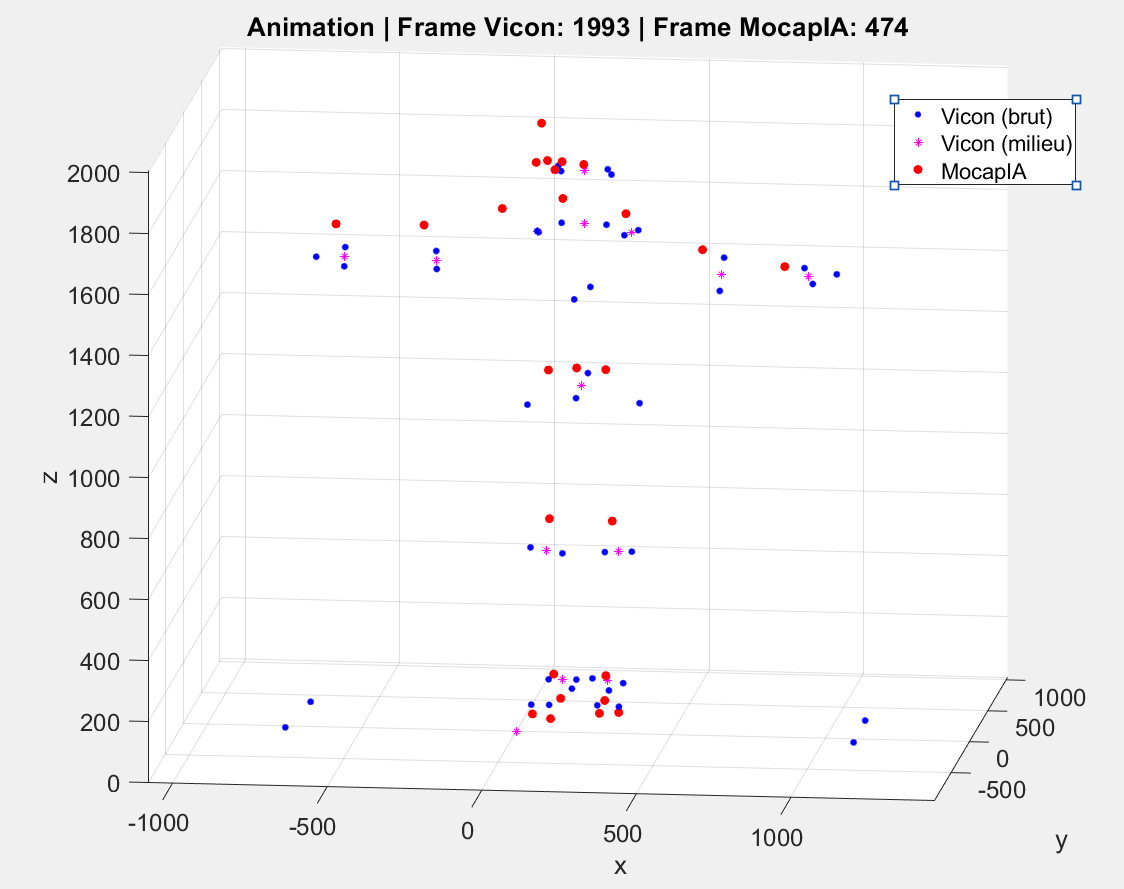
\includegraphics[width=\textwidth]{assets/Capture d'écran process/TX_ViconVSMocapIA/vicon_mocap_superpose.png}
        \caption{Superposition des points caractéristiques MoCapIA et Vicon pour l'étude qui va suivre}
        \label{fig:superposition_vicon_mocapia}
    \end{figure}

    Choisit par les TX comme un mouvement impliquant le haut du corps comme le bas, une séquence de quatre jumpings jacks à différentes vitesses a été enregistrée simultanément par le système Vicon et par le système MoCapIA.
    Venant de deux systèmes différents, les données doivent être synchronisées. Lors de chaque vidéo, le sujet part d'une \textit{T-pose} (position en T), effectue un "clap" avec les mains et en repérant la distance minimum entre les deux poignets, le système est capable d'initialiser un nouveau $t_{0}$ (voir figure \ref{fig:before_sync} et \ref{fig:sync}). 
    
    \begin{figure}[H]
    \centering
    % Première sous-figure
    \begin{subfigure}{\textwidth}
        \centering
        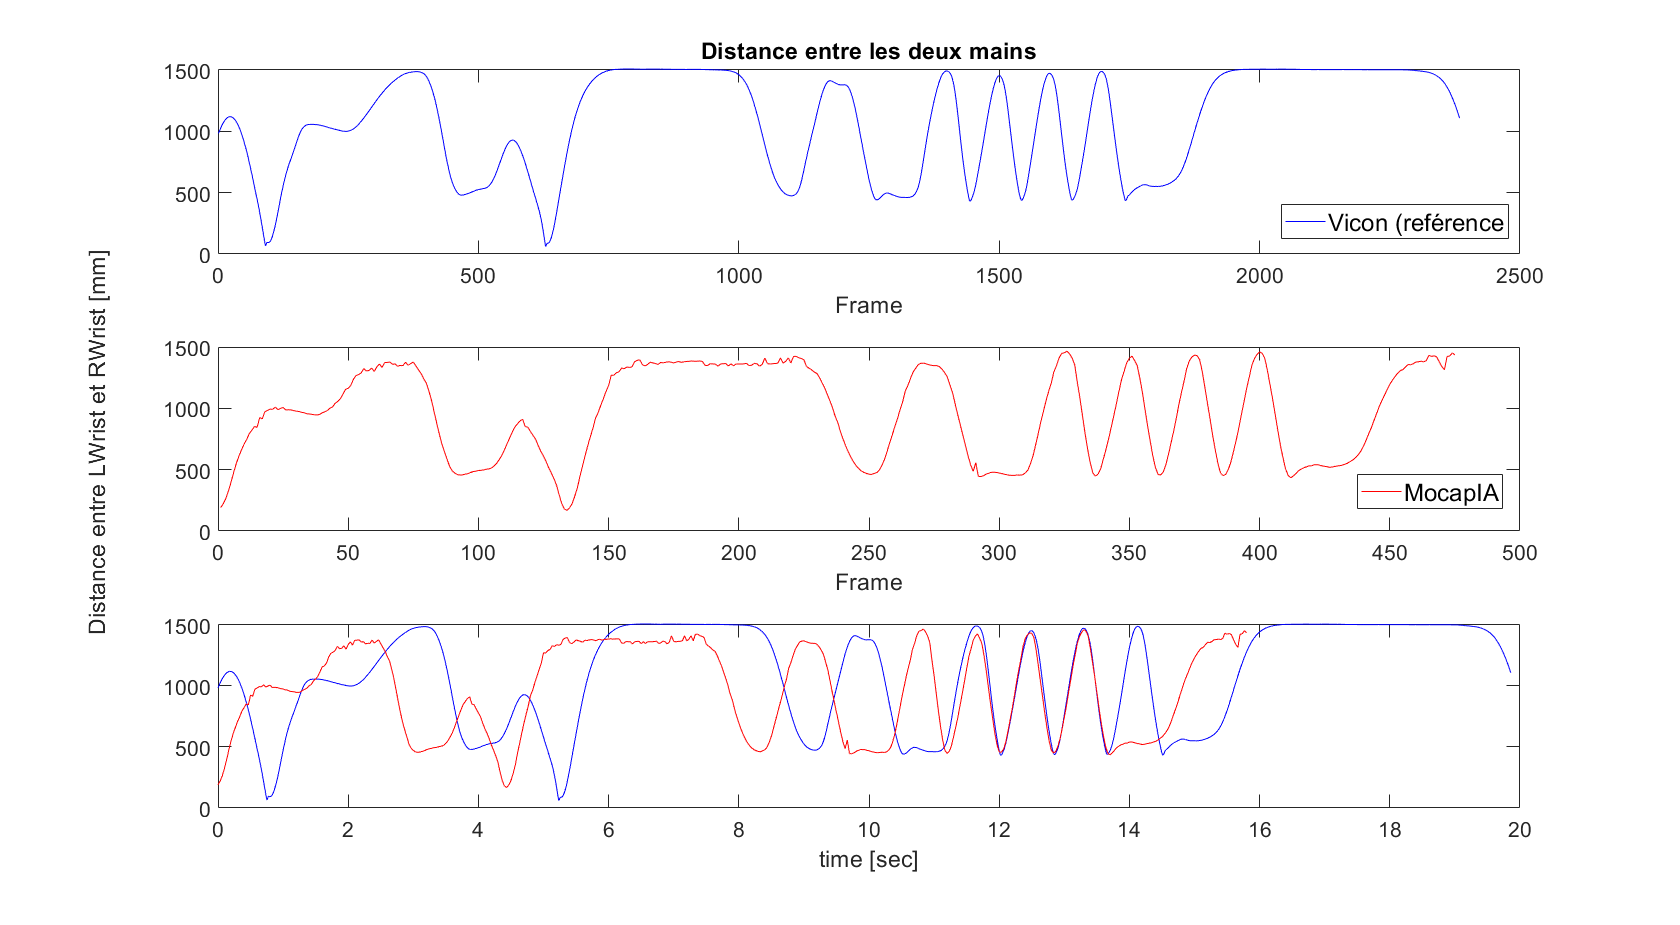
\includegraphics[width=\linewidth]{assets/Capture d'écran process/TX_ViconVSMocapIA/before_sync.png}
        \caption{Avant synchronisation}
        \label{fig:before_sync}
    \end{subfigure}
    
    % On met la légende principale ici (ou sur la 2ème partie, au choix)
    \caption{Synchronisation des données Vicon et MoCapIA (début)}
    \label{fig:sync}
\end{figure}

\begin{figure}[H]
    \ContinuedFloat
    \centering
    % Deuxième sous-figure
    \begin{subfigure}{\textwidth}
        \centering
        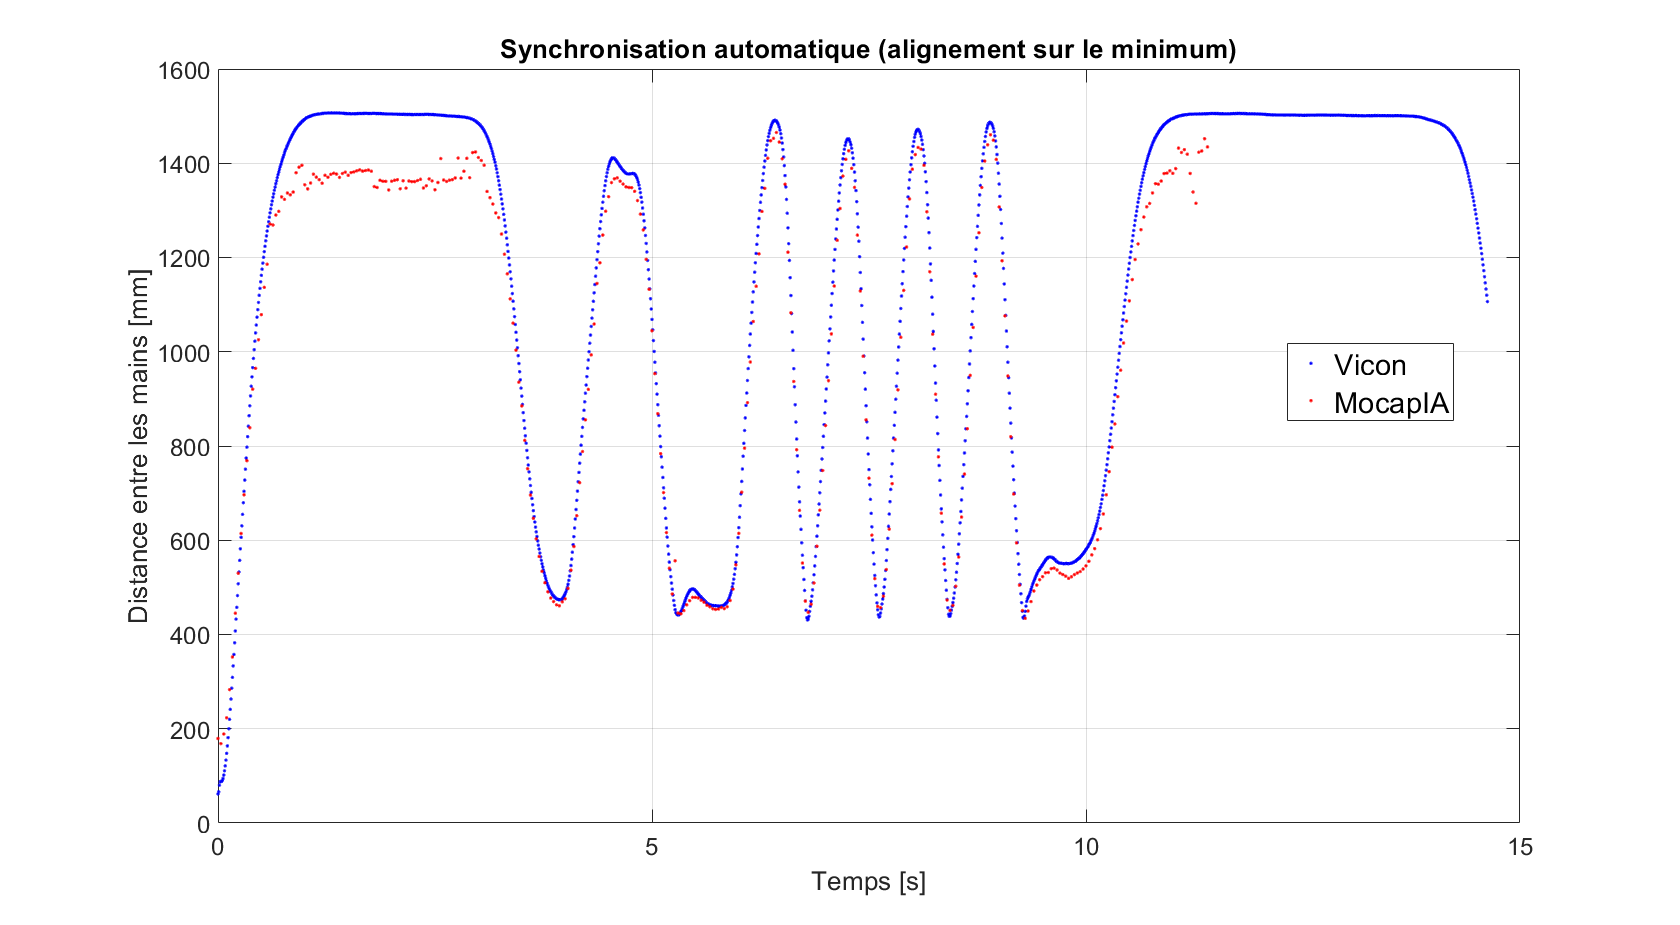
\includegraphics[width=\linewidth]{assets/Capture d'écran process/TX_ViconVSMocapIA/sync.png}
        \caption{Synchronisation appliquée}
        \label{fig:after_sync}
    \end{subfigure}
    
    \caption{Synchronisation des données Vicon et MoCapIA (suite)}
\end{figure}
    
    Ensuite pour chaque articulation notée de 1 à 21, il est nécessaire de calculer déjà l'écart entre les deux systèmes sur l'ensemble des frames. Un "offset" est obligatoirement présent, car les deux systèmes ne placent pas les points caractéristiques exactement au même endroit (ex : le marqueur physique de l'épaule du système Vicon est placée plus en arrière que le marqueur virtuel de l'épaule du système MoCapIA). Pour connaître la précision de notre système par rapport à celui du Vicon, il a été décidé d'ignorer l'offset afin de se concentrer sur la variation des mesures. Ainsi, pour chaque articulation, on calcule la moyenne et l'écart type des erreurs entre les deux systèmes (voir figure \ref{fig:mean_sd_vicon_mocapia}). Ici la moyenne n'a pas vraiment de sens, car elle correspond à l'offset en moyenne au cours du temps. Pour la tête (indice n°13), l'offset est conséquent, parce que le point caractéristique du MoCapIA est situé sur le haut du crâne tandis que le Vicon place le point au centre de la tête, soit un écart de $20cm$. Pour autant des différences sont à noter suivant l'articulation examinée. Les écarts types varient de $8mm$ pour des articulations comme les épaules à $34mm$ pour des points comme la tête ou les poignets. La moyenne des écarts types sur l'ensemble des articulations est de $15.6mm$, autrement dit environ $68\%$ varient dans l'intervalle $[ \text{offset} -15.6mm ; \text{offset} +15.6mm ]$. 
    \begin{figure}[H]
        \centering
        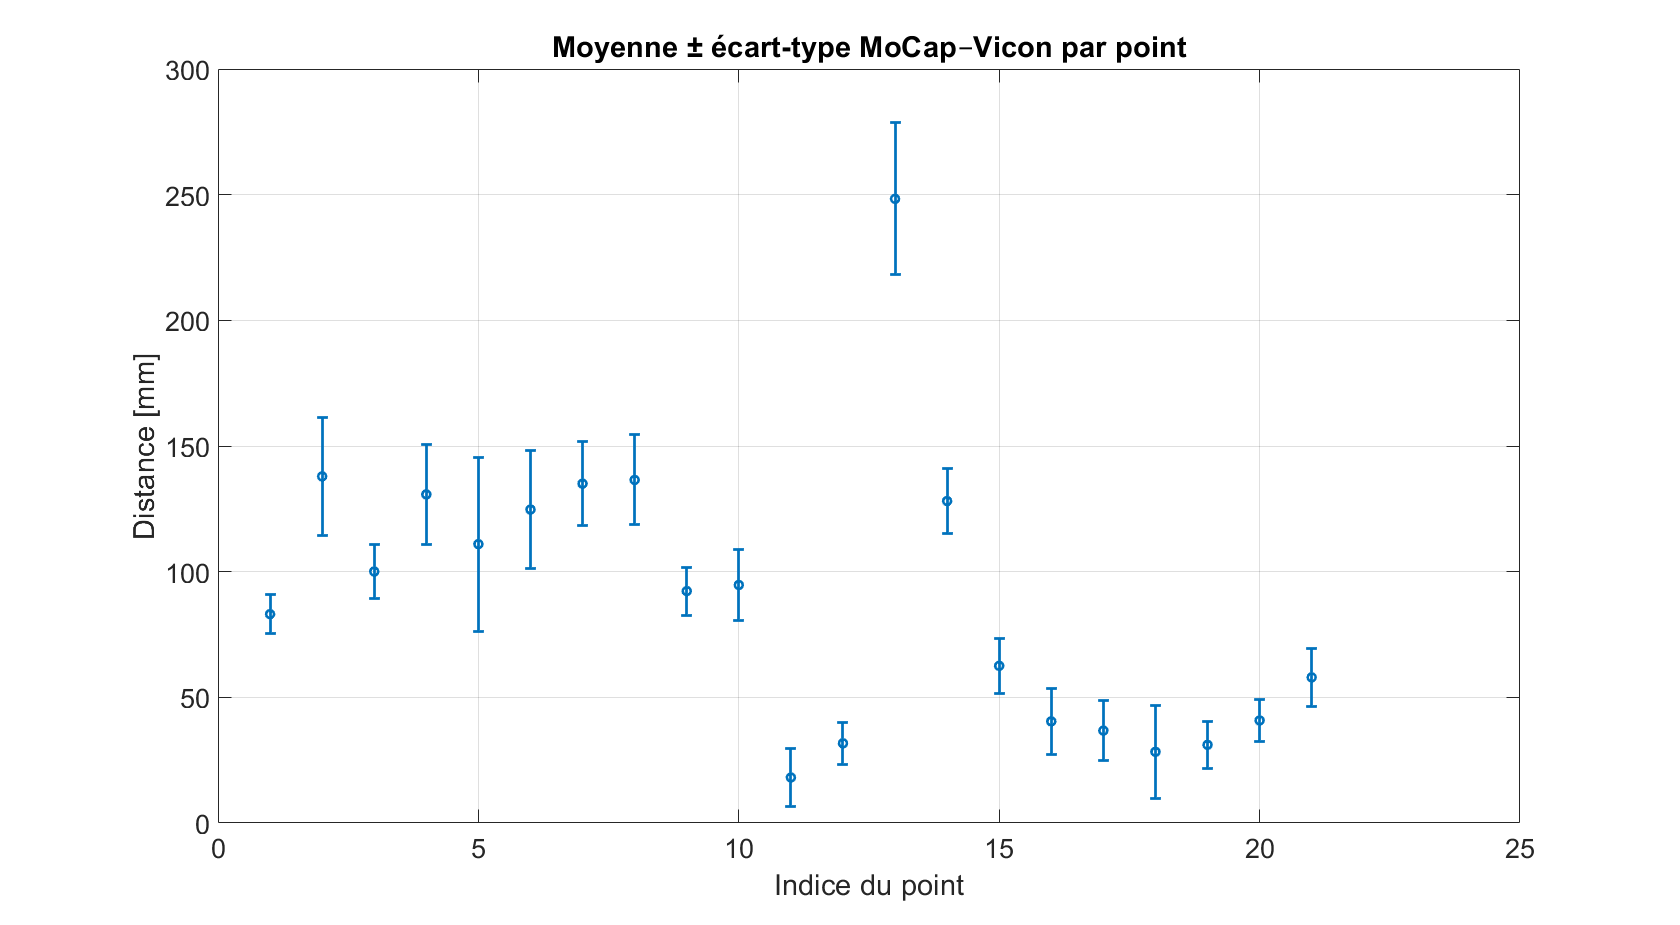
\includegraphics[width=\textwidth]{assets/Capture d'écran process/TX_ViconVSMocapIA/mean_sd_result.png}
        \caption{Moyenne et écart type des erreurs entre Vicon et MoCapIA pour les 21 articulations}
        \label{fig:mean_sd_vicon_mocapia}
    \end{figure}

    Il est intéressant d'utiliser les boxplots (figure \ref{fig:boxplot_vicon_mocapia}) afin de mettre en avant la plage de variation des erreurs (plus représentatif de la stabilité ou non du système que l'écart type). La majorité des mesures, représentée par l'étendue des moustaches (1,5 × écart interquartile), se situe dans une plage de fonctionnement de $57.40 mm$ en moyenne. Cette méthode exclut les valeurs aberrantes, mais restent fidèles au fonctionnement global du système. Même si cette valeur moyenne semble assez faible donc satisfaisante, certaines articulations présentent des plages de variations bien plus importantes. On observe deux situations. La première se trouve au niveau des articulations sensibles du haut du corps, comme les poignets et la tête avec respectivement une variation de $143mm$, $114mm$ et $127mm$. Pour le bas du corps, notamment pour les orteils et le talon, la plage de fonctionnement est bien plus petite ($\approx 30mm$) mais le nombre de valeurs aberrantes est bien plus important en représentant en moyenne $15\%$ des valeurs totales. Au contraire, pour les articulations du haut du corps, on obtient une plage de fonctionnement bien plus grande ($\approx 80mm$) mais avec un pourcentage de valeurs aberrantes inférieures $0 \text{ à } 2\%$ sur l'ensemble des valeurs \cite{OpticalMoCapLongo}.
    \begin{figure}[H]
        \centering
        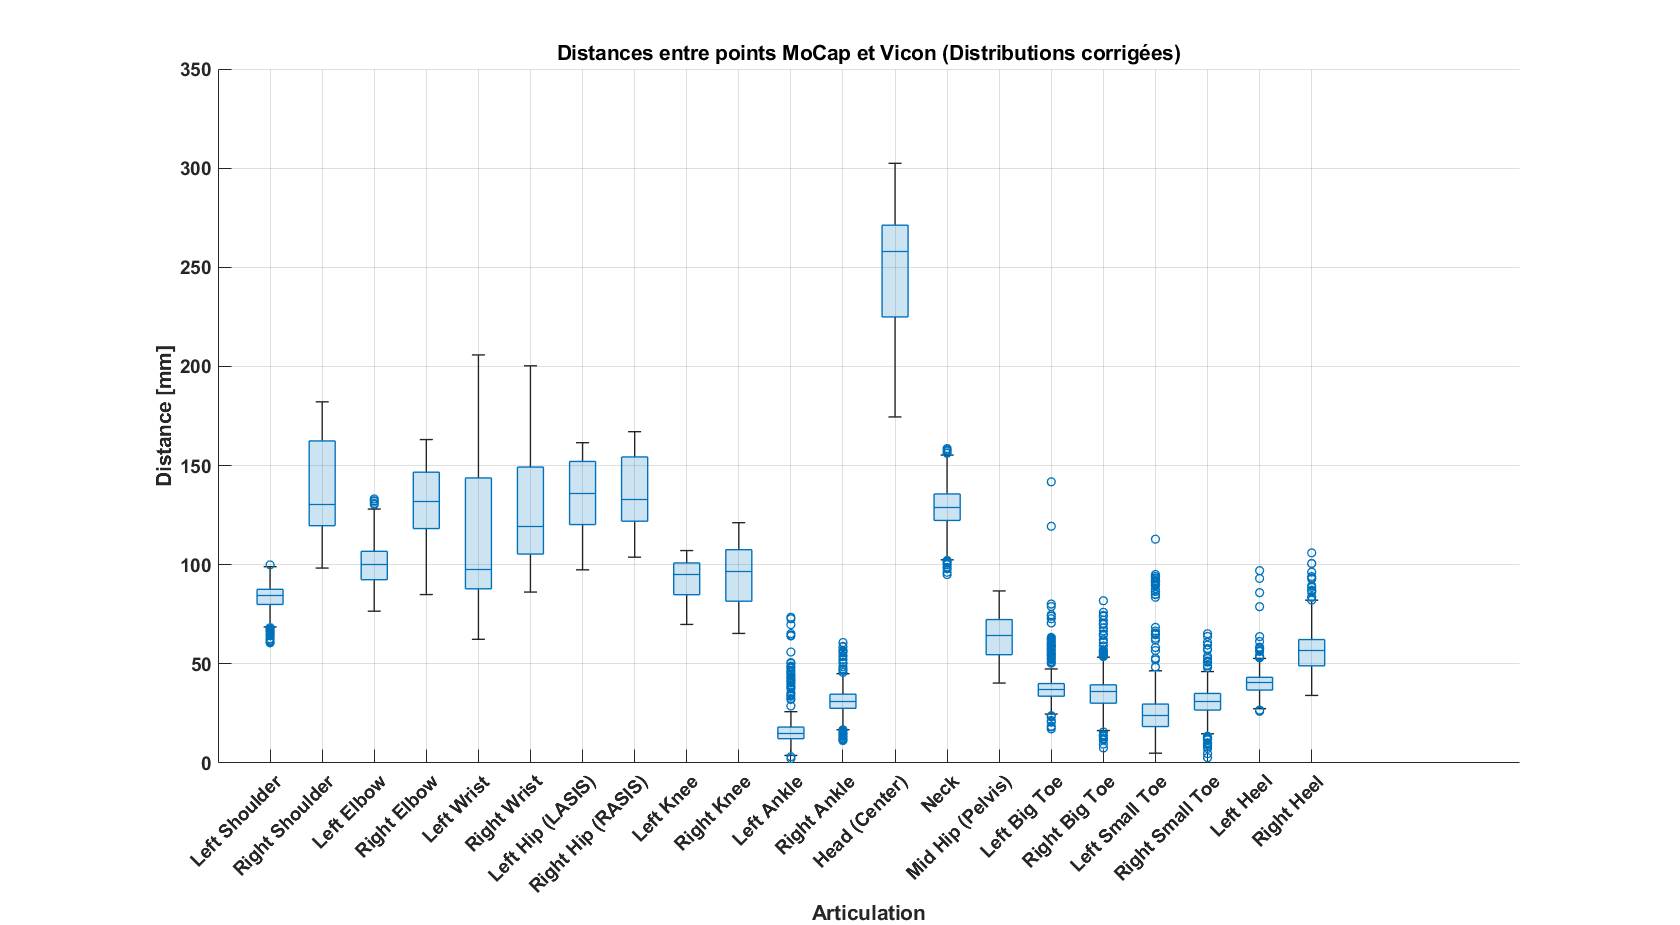
\includegraphics[width=\textwidth]{assets/Capture d'écran process/TX_ViconVSMocapIA/boxplot_vicon_mocap.png}
        \caption{Boxplots des erreurs entre Vicon et MoCapIA pour chaque articulation}
        \label{fig:boxplot_vicon_mocapia}
    \end{figure}

    Il est pertinent d'ajouter l'analyse Bland-Altman afin de comparer la validité de MoCapIA par rapport au système Vicon. Là encore le biais (erreur systématique/constante) représente la différence de positions entre les marqueurs physiques du Vicon et les marqueurs virtuels du modèle utilisé par MoCapIA. La variation aléatoire représente les erreurs réelles de MoCapIA. Les résultats sont bons, avec $\approx 95\%$ des valeurs situées entre $122.2mm$ et $80.2mm$ ($\text{mean} \pm1.96*\text{SD}$).
    \begin{figure}[H]
        \centering
        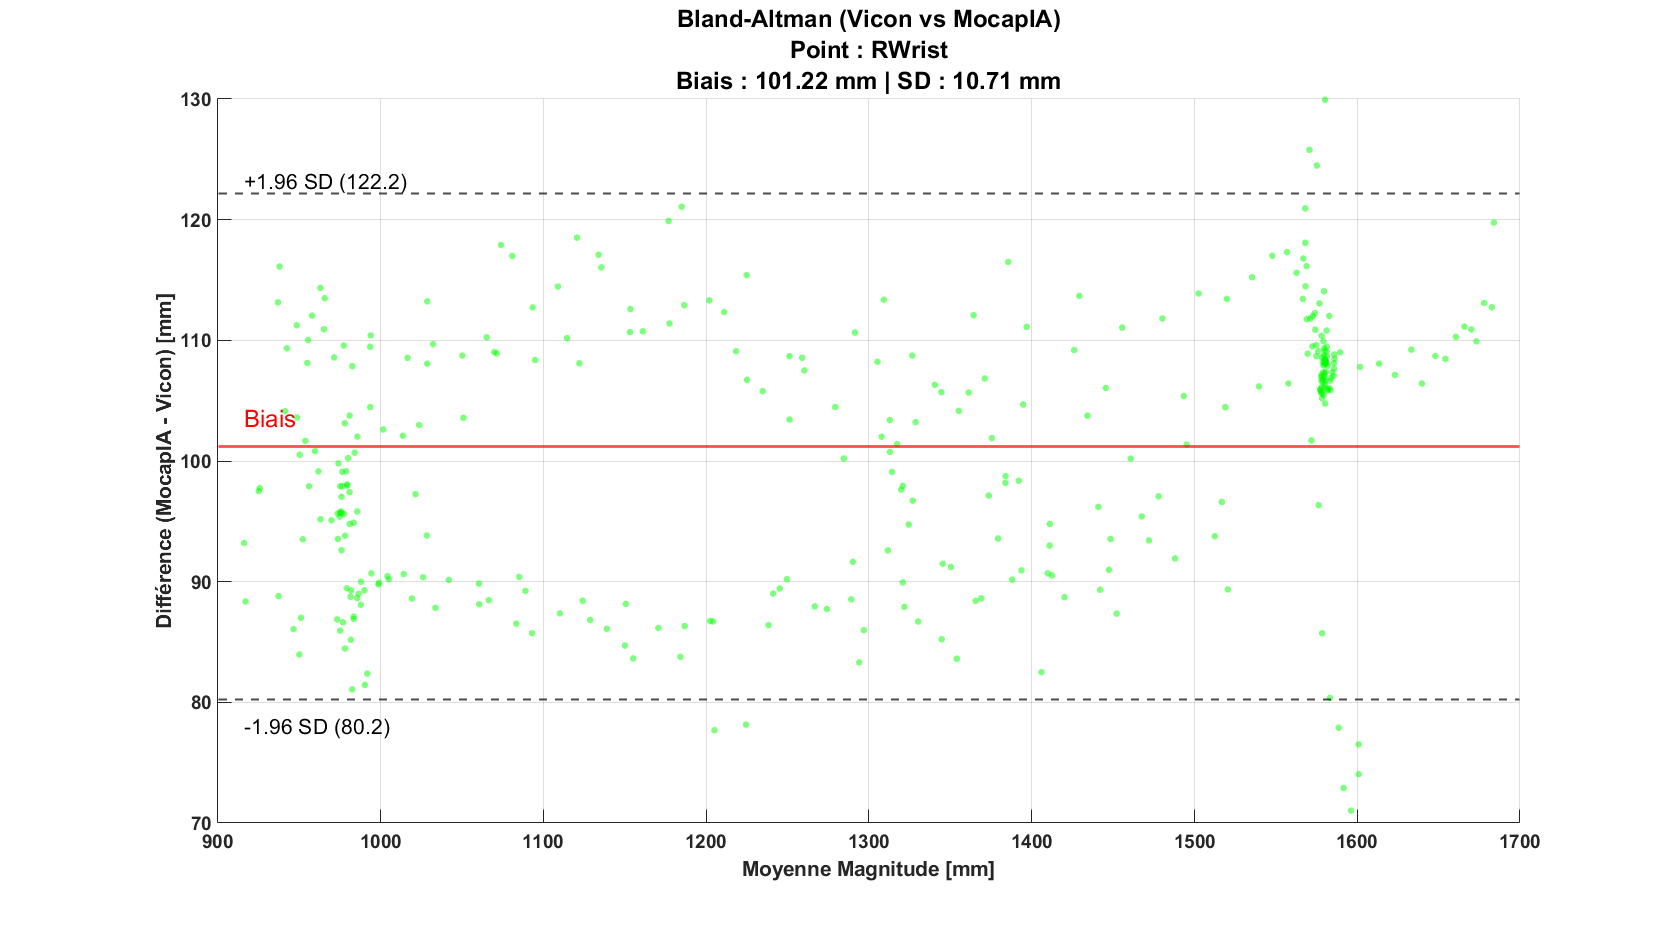
\includegraphics[width=\textwidth]{assets/Capture d'écran process/TX_ViconVSMocapIA/BlandAltman_Vicon_Mocap.png}
        \caption{Analyse Bland-Altman entre Vicon et MoCapIA pour le poignet Droit}
        \label{fig:bland_altman_vicon_mocapia}
    \end{figure} 

    Maintenant que l'analyse de l'erreur de position est faite, il est intéressant d'effectuer une analyse cinématique (angulaire) pour étudier la cohérence biomécanique et l'utilité clinique. Pour ça on utilise le produit scalaire de deux scalaires. Pour trouver l'angle $\theta$ au sommet $B$ formé par les points $A$, $B$ et $C$, on utilise la formule suivante :
    \begin{equation}
        BA \cdot BC = ||BA|| \cdot ||BC|| \cdot \cos(\theta)
    \end{equation}
    Ainsi, on obtient l'angle $\theta$ :
    \begin{equation}
        \theta = \arccos\left(\frac{BA \cdot BC}{||BA|| \cdot ||BC||}\right)
    \end{equation}

    La métrique la plus répandue dans le domaine biomécanique est la RMSE (Root Mean Square Error). En considérant toujours Vicon comme la référence, elle se calcule de cette façon :
    \begin{equation}
        RMSE = \sqrt{\frac{1}{N} \sum_{i=1}^{N} ( \theta_{Vicon}(i) - \theta_{MoCapIA}(i) )^2 }
    \end{equation}
    Avec :
    \begin{description}
        \item[$\theta_{Vicon}(i)$] l'angle mesuré par le système Vicon à la frame $i$
        \item[$\theta_{MoCapIA}(i)$] l'angle mesuré par le système MoCapIA à la frame $i$
        \item[$N$] le nombre total de frames
    \end{description}
    Les résultats montre une bonne performance du système MoCapIA avec une RMSE de $5.28^\circ$ pour le coude gauche et de $2.0^\circ$ pour le genou gauche. Les résultats sont satisfaisants, étant donné que d'après la littérature, les meilleurs résultats obtenus avec des systèmes markerless atteignent une RMSE d'environ $3.5^\circ$ pour des mouvements simples \cite{LSTM}. 

    \begin{figure}[H]
        \centering
        
\includegraphics[width=\textwidth]{assets/Capture d'écran process/TX_ViconVSMocapIA/angle_CoudeG.png}
        \caption{RMSE de l'angle du coude gauche entre Vicon et MoCapIA}
        \label{fig:angle_coudeG}
    \end{figure}

    D'autres résultats secondaires ont été obtenus durant ce test, et sont présentés en Annexe \ref{AnnexVicon_Mocap}.

    En conclusion, l'estimation 2D engendre la majeure partie des erreurs totales du système avec des autres de grandeurs atteignant la dizaine de centimètres pour certaines articulations. La calibration et la triangulation n'engendrent que très peu d'erreurs à comparer, avec des erreurs moyennes de l'ordre du centimètre. Les erreurs de ces modèles d'IA open-source comme celui utilisé (RTMPose) comportent des erreurs à la fois à cause des données d'entraînement pas totalement adaptées à la biomécanique et des problèmes d'occultation durant l'entraînement \cite{MarkerlessforBiomecha}. D'un autre côté, il est pourtant important de notifier que la précision angulaire de MoCapIA est satisfaisante par rapport à sa précision de position. C'est donc sur ce premier point que la suite des réalisations va se concentrer.

\section{Amélioration du processus MoCapIA}

    À ce stade du stage, l'estimation 2D est identifiée comme la principale source d'erreurs du système MoCapIA. Ces erreurs empêchent une analyse biomécanique sérieuse et fiable. De plus le problème auquel il faut faire face est le suivant : \textbf{RTMPose} (modèle de détection des articulations) est le modèle OpenSource \textbf{le plus précis actuellement disponible} pour une estimation 2D du corps humain assez rapide \cite{HumanPoseEstimationModels}\cite{RTMPose}. Les solutions open-source souffrent de négligence durant l'entraînement, c'est de là que viennent les erreurs importantes \cite{MarkerlessforBiomecha}. Il est donc nécessaire d'ajouter des étapes supplémentaires au processus MoCapIA pour corriger les erreurs restantes.

    Après plusieurs recherches, un module OpenSource appelé \textbf{Pose2Sim} a été trouvé. Ce module reprend en partie le processus MoCapIA mais ajoute des étapes supplémentaires conçues pour l'analyse biomécanique. En effet, en plus d'effectuer une calibration, une estimation 2D et une reconstruction 3D simple, Pose2Sim ajoute un processus de filtrage, une augmentation du nombre de marqueurs ainsi qu'une correction biomécanique des mouvements. L'ajout de marqueurs virtuels permettrait d'utiliser ce package \textit{opensim} et le logiciel OpenSim, qui pourront eux-mêmes corriger les erreurs restantes après le filtrage et apporter les informations manquantes pour une analyse plus poussée. Ce module utilise d'ailleurs \textbf{RTMLib} pour la détection des points caractéristiques, qui appartient à la même famille que \textbf{RTMPose} (le modèle utilisé par MoCapIA).
    \begin{figure}[H]
        \centering
        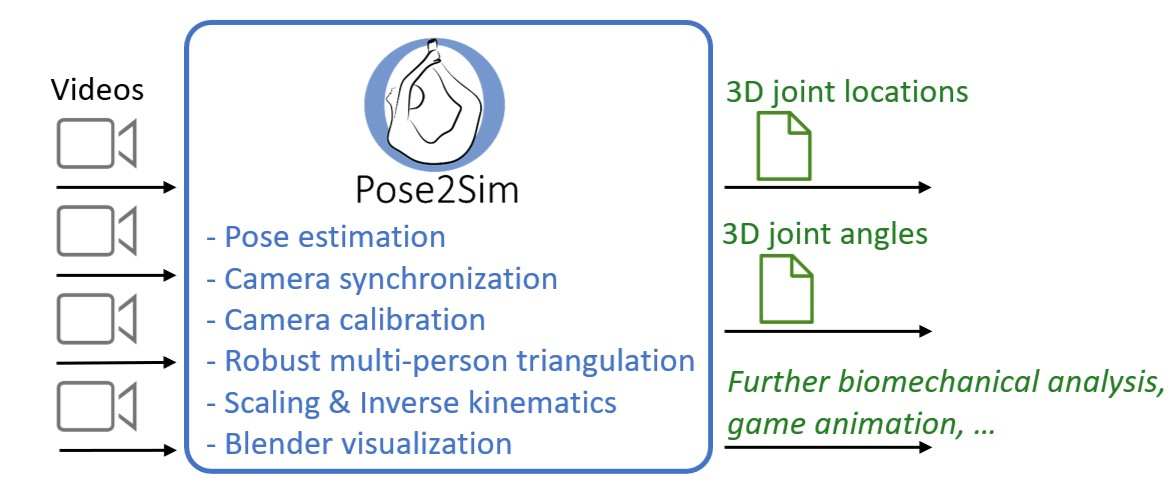
\includegraphics[width=0.8\linewidth]{assets/Capture d'écran process/Pose2Sim/Pose2Sim_workflow.jpg}
        \caption{Processus Pose2Sim (source : \href{https://github.com/perfanalytics/pose2sim}{GitHub Pose2Sim})}
        \label{fig:pose2sim_workflow}
    \end{figure}
    
    Mais avant d'implémenter ces nouvelles étapes, il est important de comparer les étapes communes entre MoCapIA et Pose2Sim (calibration, estimation 2D et triangulation) pour s'assurer de garder la version la plus précise. Pour ça, on compare les longueurs des membres du corps sur l'ensemble du mouvement. La stabilité fait aussi partie des paramètres qui seront analysés. En comparant les deux fichiers .csv de points 3D, on peut ainsi calculer sur l'ensemble du mouvement la longueur de chaque membre du corps. Sur la figure \ref{fig:boxplot_p2s_mocap}, la stabilité moyenne de Pose2Sim est supérieur, ce qui s'explique par le fait que les données de Pose2Sim dispose d'un filtrage. D'ailleurs le nombre d'outliers est plus important pour le système MoCapIA.
    \FloatBarrier
    \begin{figure}[H]
        \centering
        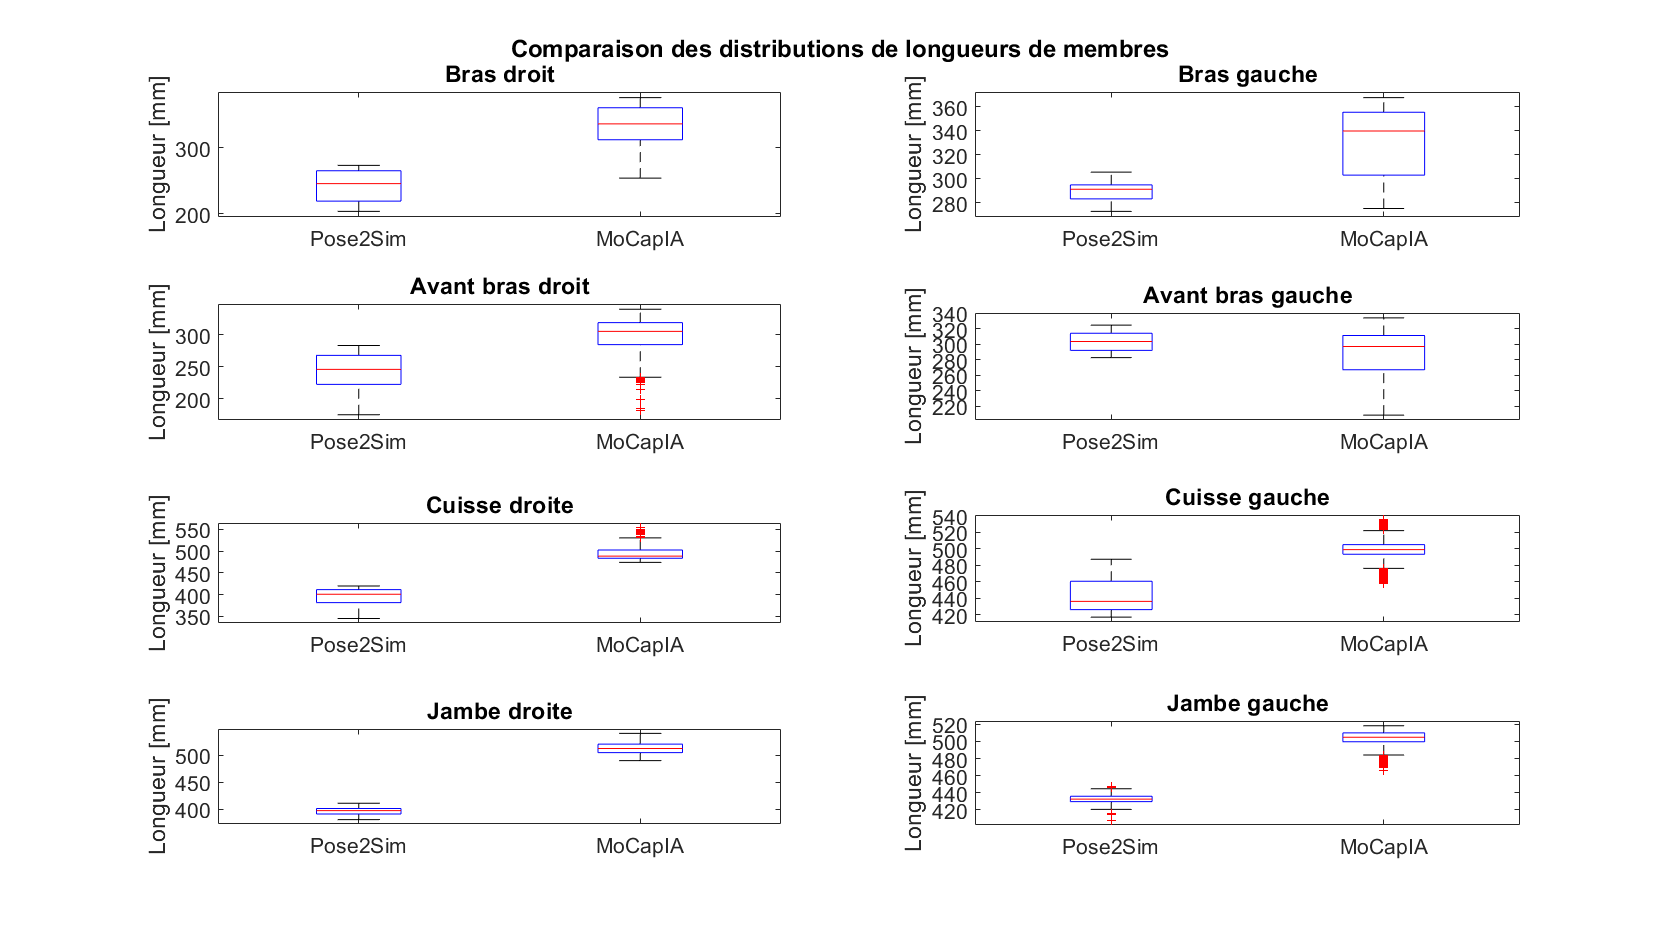
\includegraphics[width=\linewidth]{assets/Capture d'écran process/Pose2Sim/boxplot_P2S_Mocap.png}
        \caption{Comparaison des distributions de la longueur des membres entre Pose2Sim et MoCapIA}
        \label{fig:boxplot_p2s_mocap}
    \end{figure}
    
    \FloatBarrier
    D'un autre côté, les deux systèmes utilisent le même modèle de squelette (Halpe26 : figure \ref{fig:halpe26}) ; il est donc possible, à l'aide des longueurs théoriques mesurées sur le sujet, de comparer la précision des deux systèmes. 
    
    \begin{table}[h!]
    \centering
    \renewcommand{\arraystretch}{1.5}
    \begin{tabularx}{\textwidth}{|l|>{\centering\arraybackslash}X|>{\centering\arraybackslash}X|>{\centering\arraybackslash}X|} 
        \hline
         & \textbf{Longueur bras gauche} & \textbf{Longueur bras droit} & \textbf{Erreur moyenne (ensemble)}\\
        \hline
        Mesure théorique & $290mm$ & $290mm$ & x \\
        \hline
        Moyenne Pose2Sim & $288.37mm$ & $243.80mm$ & $44.4mm$ \\
        \hline
        Moyenne MoCapIA & $301.46mm$ & $284.90mm$ & $23.3mm$ \\
        \hline
    \end{tabularx}
    \caption{Comparaison des différents systèmes de caméras}
    \label{tab:cameras}
\end{table}

    Finalement l'erreur moyenne des membres par rapport aux valeurs théoriques du  processus MoCapIA est inférieur à celle de Pose2Sim. C'est donc ce pipeline qui sera conservé pour la suite du projet. Pour autant, il est nécessaire de filtrer nos valeurs et d'ajouter les étapes suivantes (augmentation de marqueurs et correction biomécanique) qui vont être testées et implémentées ci-dessous.

\section{Implémentation du filtrage}

    Même si Pose2Sim n'est pas aussi juste que MoCapIA sur la construction d'un modèle 3D simple, la figure \ref{fig:boxplot_p2s_mocap} montre que MoCapIA obtient plus de valeurs aberrantes (croix rouges sur le graphique). Pour réduire ces erreurs, il est possible d'implémenter des filtres sur les données 3D. Plusieurs types de filtres sont disponibles dans le package Pose2Sim. Il a donc été décidé de tous les tester pour déterminer lequel est le plus adapté aux données biomécaniques issues de MoCapIA. Les filtres testés sont les suivants :
    \begin{itemize}
        \item Filtre LOESS
        \item Filtre Gaussian
        \item Filtre GCV Spline
        \item Filtre Butterworth Speed
        \item Filtre Kalman
        \item Filtre Butterworth Classique
        \item Filtre Hampel
    \end{itemize}
    Les 2 derniers filtres sont ceux qui ont été garder après leur étude (les autres résultats sont présentés en Annexe \ref{Annexfiltres}). En effet, les autres ne sont pas adaptés aux signaux biomécanique à l'inverse du filtre Butterworth \cite{FiltresComparaison}\cite{Butter}\cite{Butter2}. Le filtre \textit{Hampel} est un filtre de détection de valeurs aberrantes qui a été ajouté en amont des autres filtres pour améliorer leur efficacité. Voici son impact sur l'articulation LWrist (poignet gauche), l'une des articulations la plus sujette aux erreurs :
    \begin{figure}[H]
        \centering
        \begin{subfigure}{\textwidth}
            \centering
            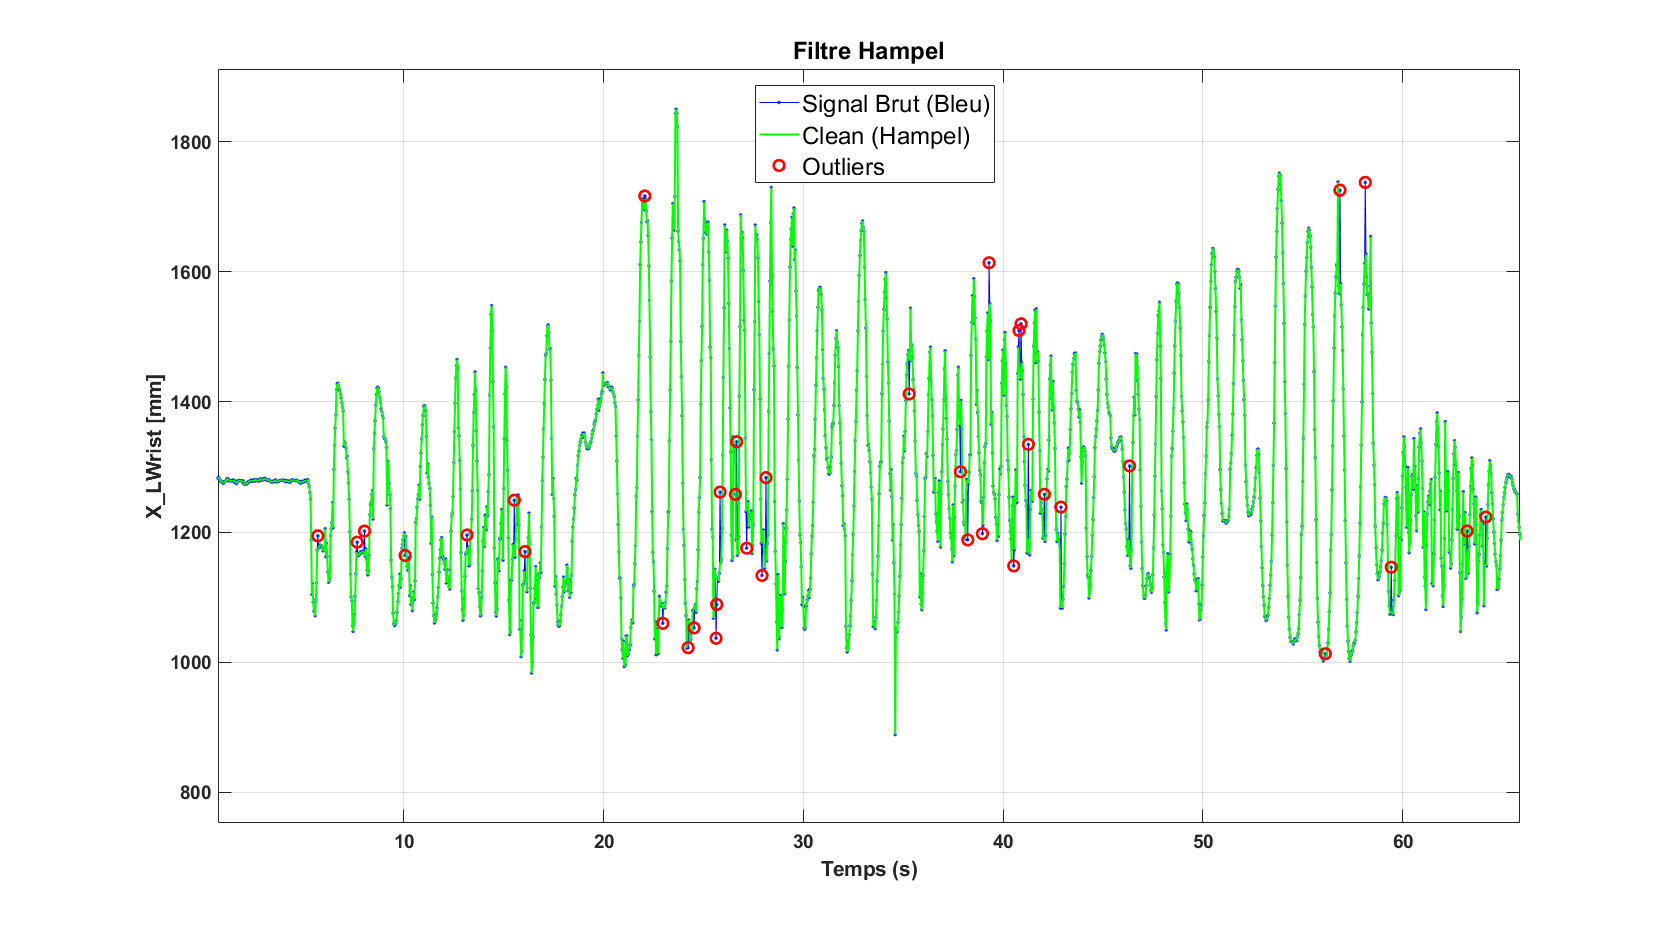
\includegraphics[width=\textwidth]{assets/Capture d'écran process/Tests Filtres 3D/valid/hampel.png}
            \caption{Filtrage Hampel appliqué}
            \label{fig:filtre_hampel}
        \end{subfigure}
        \hfill
        \begin{subfigure}{\textwidth}
            \centering
            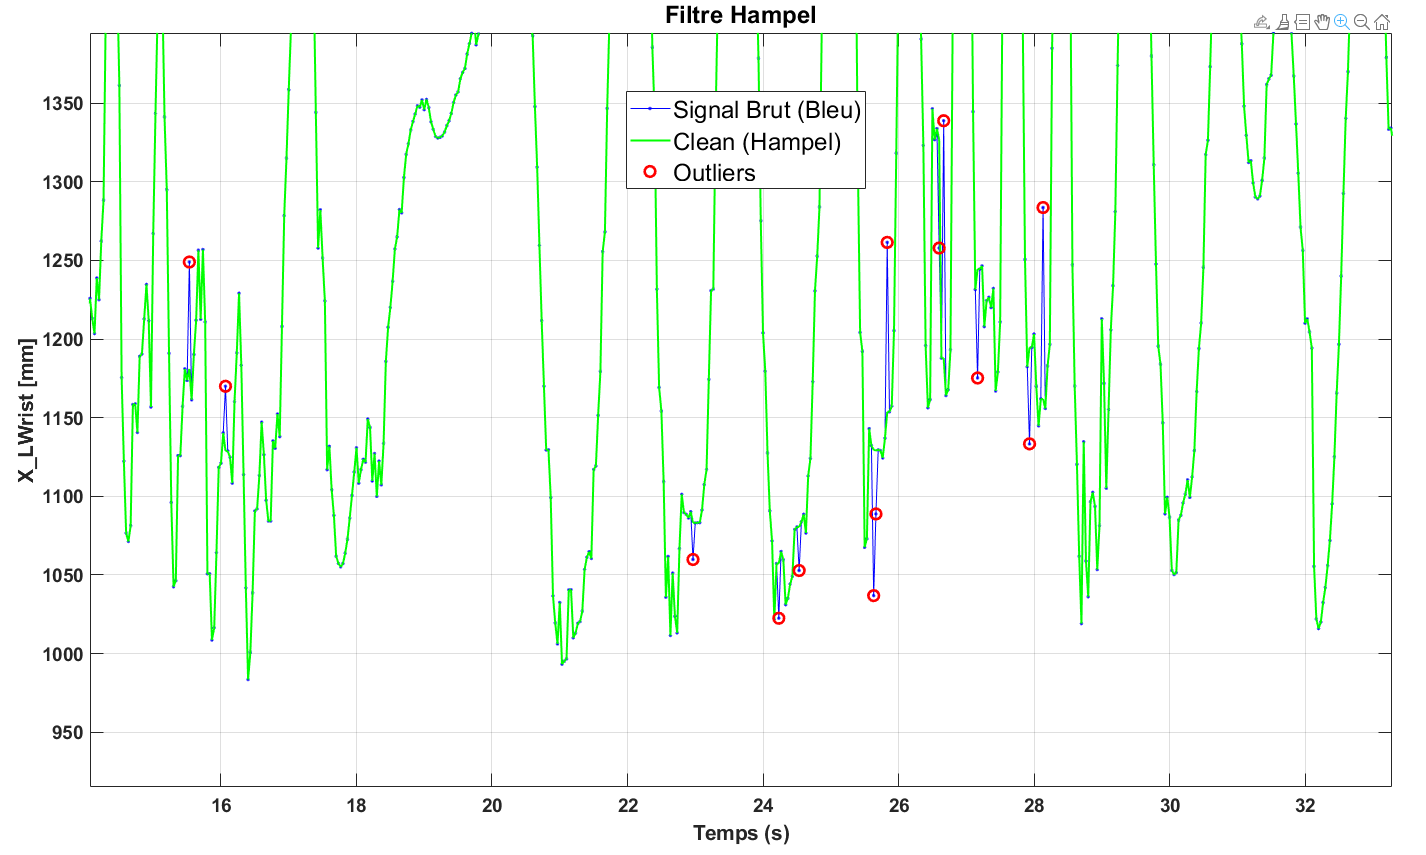
\includegraphics[width=0.8\textwidth]{assets/Capture d'écran process/Tests Filtres 3D/valid/hampel_zoom.png}
            \caption{Zoom sur l'action du filtre Hampel}
            \label{fig:filtre_hampel_zoom}
        \end{subfigure}
        \caption{Impact du filtre Hampel sur le signal du poignet gauche}
        \label{fig:filtre_hampel_total}
    \end{figure}

    Une fois les valeurs aberrantes supprimées, les autres filtres sont appliqués. Le filtre butterworth est un filtre numérique récursif très répandu dans le domaine biomécanique grâce à la simplicité de son écriture mathématique et de calcul. Il dépend du choix de la fréquence de coupure $f_c$ et de l'ordre $n$. La fréquence typique choisie pour le filtrage des signaux biomécaniques est de $f_c = 6$ à $10 Hz$ et l'ordre est souvent compris entre $2$ et $4$ \cite{Biblio_Filtrage1990}\cite{Butter}\cite{Butter2}. C'est celui qui a été intégré au processus.

    \begin{figure}[H]
        \centering
        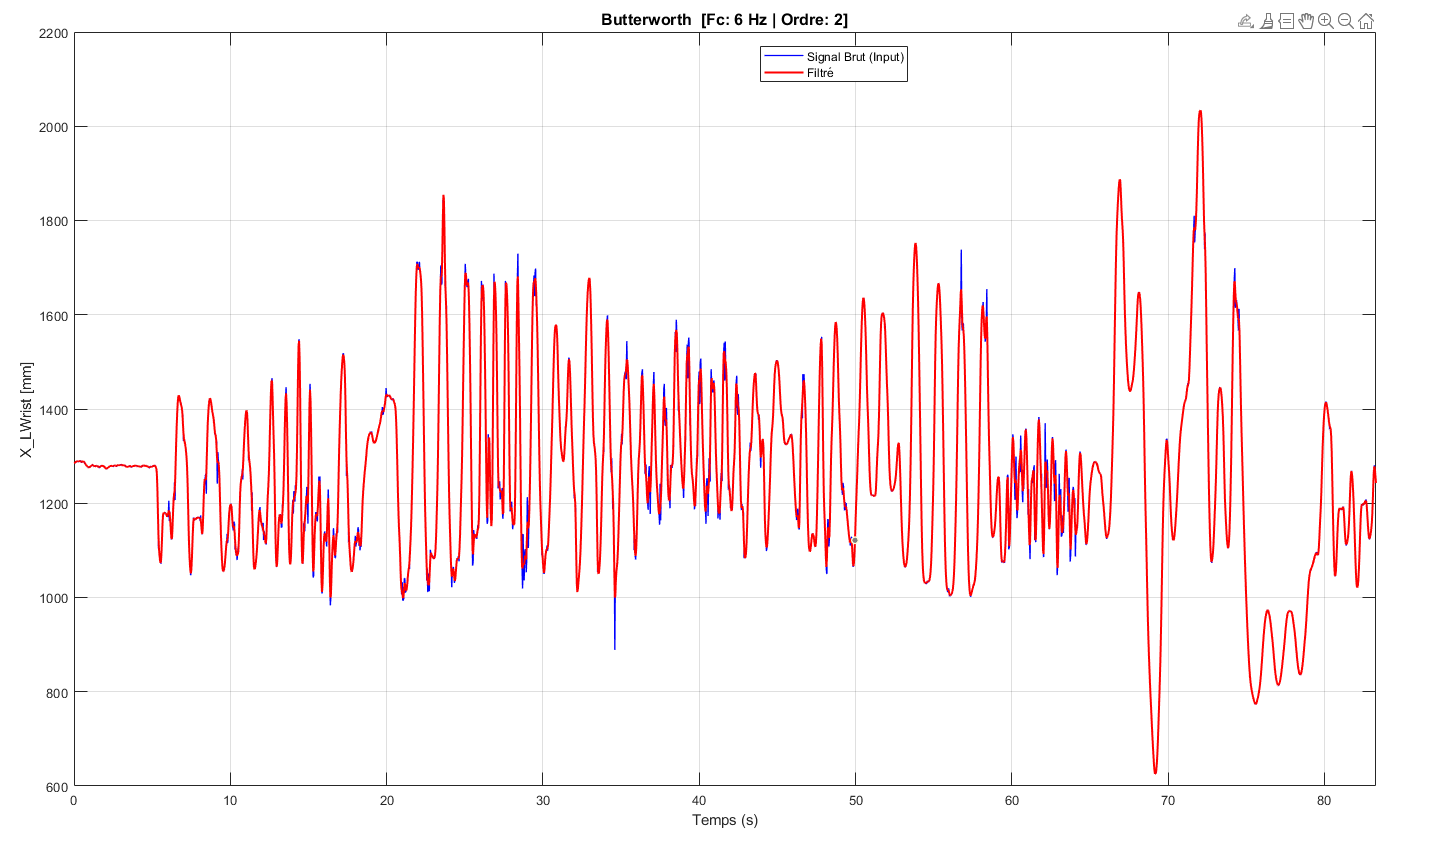
\includegraphics[width=\textwidth]{assets/Capture d'écran process/Tests Filtres 3D/valid/butterworth.png}
        \caption{Impact du filtre Butterworth sur le signal du poignet gauche}
        \label{fig:filtre_butterworth}
    \end{figure}
    Sur la figure ci-dessus, il n'est pas facile de valider le filtre. Pour ça, on applique la méthode de Bland-Altman qui permet de comparer deux séries de données. En comparant les données brutes et les données filtrées, on observe que la majorité des points ($\approx 95\%$) se situent dans les limites de concordance ($\text{mean} \pm1.96*\text{SD}$) ce qui valide l'efficacité du filtre.
    \begin{figure}[H]
        \centering
        
\includegraphics[width=\textwidth]{assets/Capture d'écran process/Tests Filtres 3D/valid/Bland_Altman_butterworth.png}
        \caption{Analyse de Bland-Altman entre les données brutes et les données filtrées sur la coordonnée X du poignet gauche}
        \label{fig:bland_altman_butterworth}
    \end{figure}

\section{Implémentation de l'augmentation de marqueurs}

    Avec le modèle de marqueur Halpe26, on a seulement 26 marqueurs. Ce n'est pas suffisant pour mener une étude du mouvement complète. On a donc besoin d'augmenter ce nombre de marqueurs. Il existe d'autres types de squelettes avec plus de marqueurs, mais leurs fiabilités laisse à désirer. On se penche donc sur une technique d'\textit{augmentation de marqueurs (marker augmentation)} qui consiste à utiliser un modèle d'apprentissage profond. Par l'intermédiaire d'un réseau \textit{Long Short-Term Memory (LSTM)} entraîné pour la capture la dynamique temporelle des données de mouvement, il est possible de transformer 20 keypoints provenant du modèle simpliste en un ensemble de \textbf{43 marqueurs atomiques} (voir figures \ref{fig:lstm_augmentation}, \ref{fig:halpe26_markers} et \ref{fig:lstm_markers}). 
    
    \begin{figure}[H]
        \centering
        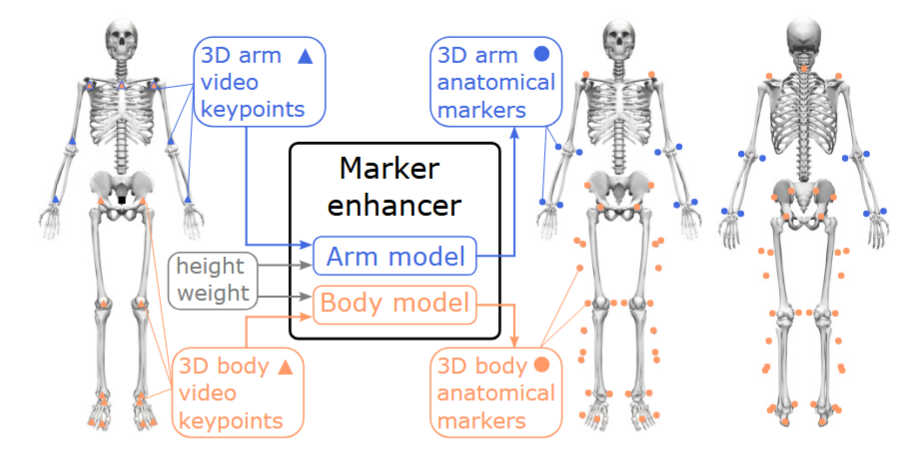
\includegraphics[width=0.8\textwidth]{assets/Capture d'écran process/Halpe26vsLSTM/LSTM.png}
        \caption{L'augmentation de marqueurs à l'aide d'un réseau LSTM (cf. \cite{LSTM})}
        \label{fig:lstm_augmentation}
    \end{figure}

    Cela est rendu possible grâce une architecture qui intègre une mémoire à long terme qui permet de conserver les informations intéressantes durant un certain temps. Contrairement aux réseaux de neurones classiques, les LSTM sont donc capables de lier les informations passées au contexte actuel. Cela permet de prédire des trajectoires fluides et cohérentes pour les nouveaux marqueurs \cite{UnderstandingLSTM}.
    \begin{figure}[H]
        \centering
        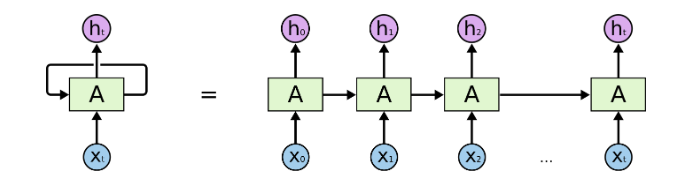
\includegraphics[width=0.8\textwidth]{assets/Capture d'écran process/Halpe26vsLSTM/LSTM_neurones.png}
        \caption{Architecture du réseau récurrent LSTM pour l'augmentation de marqueurs (cf. \cite{UnderstandingLSTM})}
        \label{fig:lstm_architecture}
    \end{figure}

    Cette technique a été implémentée à la suite du filtrage. Sur des mouvements de référence (marche, squat), l'impact de l'augmentation de marqueurs est faible, mais permet tout de même de passer d'une erreur cinématique moyenne (RMSE) de $9.6^\circ$ à $4.1^\circ$ pour les degrés de liberté rotationnels \cite{LSTM}. L'avantage majeur de l'augmentation de marqueurs est d'avoir une meilleure représentation des segments du corps humain et ainsi capturer les mouvements de rotation du bras sur lui-même par exemple. C'est donc sur les mouvements plus complexes (ex : pompes, rouler au sol) que l'augmentation de marqueurs montre tout son intérêt. En conservant une erreur moyenne de $4.1^\circ$, il surpasse largement la performance du modèle précédent (Halpe26 seul) qui atteint une erreur moyenne de $40.4^\circ$. En effet, certaines rotations ne peuvent pas être correctement estimées avec des articulations représentées seulement par un seul marqueur. 
    \begin{figure}[H]
    \centering

    \begin{subfigure}{0.48\textwidth}
        \centering
        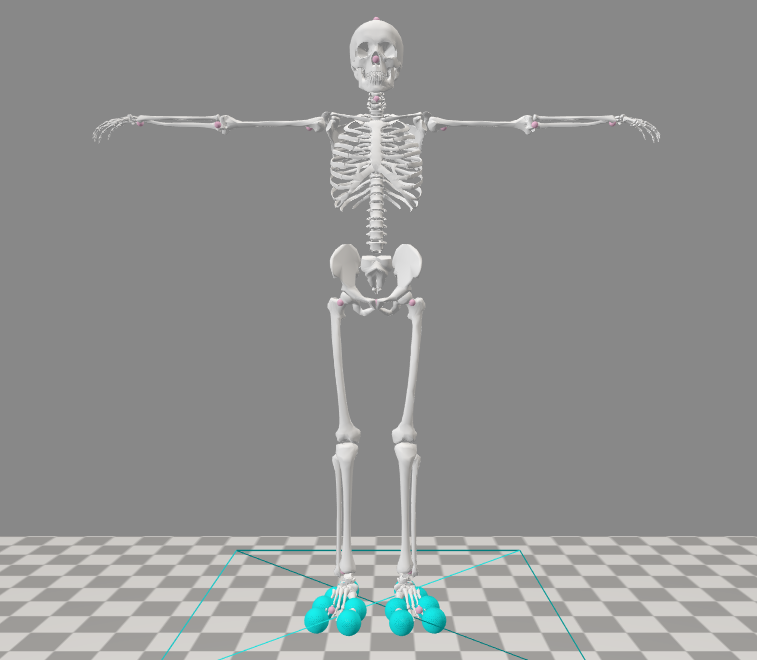
\includegraphics[width=\linewidth]{assets/Capture d'écran process/OpenSim/markerHALPE26.png}
        \caption{Squelette avec les marqueurs Halpe26}
        \label{fig:halpe26_markers}
    \end{subfigure}
    \hfill
    \begin{subfigure}{0.51\textwidth}
        \centering
        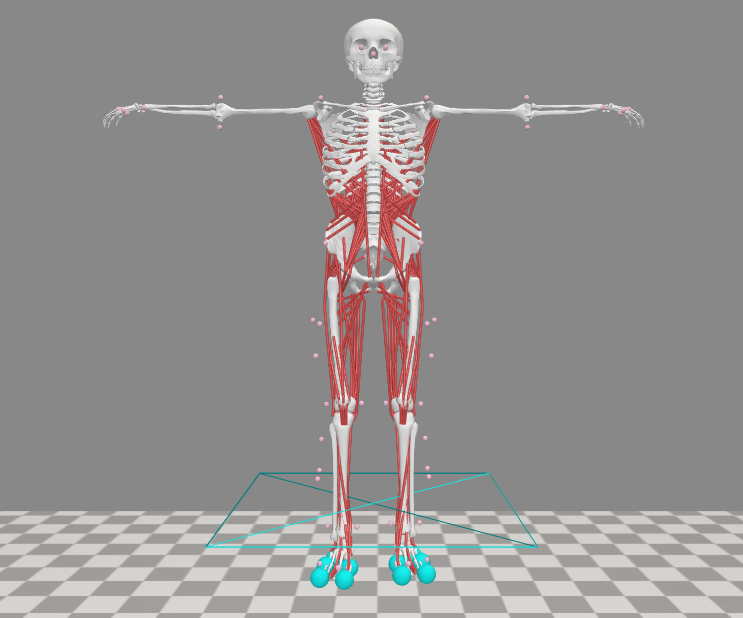
\includegraphics[width=\linewidth]{assets/Capture d'écran process/OpenSim/markeraugmented.png}
        \caption{Squelette avec l'augmentation de marqueurs}
        \label{fig:lstm_markers}
    \end{subfigure}
    
    \caption{Comparaison du squelette avant et après l'augmentation de marqueurs sur OpenSim}
    \label{fig:comparaison_marqueurs}
    \end{figure}

\section{Intégration de la correction biomécanique}
    Avec les nouveaux fichiers contenant les nouveaux marqueurs et le package \textit{opensim}, il est possible d'ajouter deux étapes de correction biomécanique.  Nous avons décomposé cette étape en deux objectifs cruciaux : le \textit{Scaling} (la mise à l'échelle) et le \textit{Kinematic Fitting} (l'ajustement cinématique).

    \subsection{\textit{\textbf{Scaling}}}
        Le \textit{\textbf{Scaling}} consiste à adapter un modèle générique d'un squelette aux dimensions de notre sujet. Cette étape est essentielle avant d'exécuter l'analyse cinématique, car chaque individu possède des proportions biomécaniques différentes. On utilise donc ce modèle $.osim$ ainsi que nos coordonnées 3D (fichier $.trc$) d'un essai statique (T-Pose). En mesurant les distances entre des paires de marqueurs (ex : \texttt{r\_knee} et \texttt{r\_ankle}), on obtient les facteurs d'échelle de chaque membre du corps.
        \begin{equation}
            fe = \frac{d_{marqueurs}}{d_{generique}}
        \end{equation}
        \begin{description}
            \item[$fe$] le facteur d'échelle
            \item[$d_{marqueurs}$] la distance mesurée entre les marqueurs de chaque membre du sujet
            \item[$d_{generique}$] la distance entre les mêmes marqueurs sur le modèle générique
        \end{description}
        Ces facteurs d'échelles vont permettre d'ajuster le modèle $.osim$ initial aux dimensions du sujet. De plus, en prenant en compte la masse du sujet donnée dans la configuration, on peut ajuster les propriétés inertielles du modèle (masse, centre de masse, moments d'inertie) en fonction des proportions du sujet. Finalement, on obtient un nouveau modèle $.osim$ avec les propriétés biomécaniques du sujet.

    \subsection{\textit{\textbf{Cinématique Inversée}}}
    La \textit{\textbf{Cinématique Inversée} (Inverse Kinematics - IK)} permet de contraindre les données à un modèle musculosquelettique, garantissant ainsi la cohérence biomécanique des mouvements. Autrement dit, on ajoute des contraintes sur les résultats obtenus précédemment et on essaie de minimiser les erreurs pour satisfaire au mieux ces contraintes. Son utilisation est reconnue dans la littérature scientifique de biomécanique \cite{LSTM}\cite{Butter2}. On va donc utiliser le modèle $.osim$ mis à l'échelle ainsi que les coordonnées 3D (fichier $.trc$) du mouvement. L'algorithme calcule de nouvelles positions pour chaque marqueur à différend angles. Cet ensemble d'angles $q$ est censé minimiser la somme des carrés des distances entre chaque marqueur expérimentaux. C'est comme ça que les angles articulaires du mouvement sont obtenus. 

    \begin{equation}
        \min_{q} \sum_{i=1}^{n} w_i \| p_{i}^{exp} - p_{i}^{sim}(q) \|^2
    \end{equation}

    \begin{description}
        \item[$w_i$] le poids attribué au marqueur $i$
        \item[$p_{i}^{exp}$] la position expérimentale du marqueur $i$
        \item[$p_{i}^{sim}(q)$] la position simulée du marqueur $i$ en fonction des angles articulaires $q$
        \item[$n$] le nombre total de marqueurs 
    \end{description}

    Les résultats obtenus après l'étape de cinématique inversée montrent une nette amélioration de la cohérence biomécanique des mouvements. En comparant les angles articulaires des marqueurs augmentés et du résultat final après la cinématique inversée et le scaling avec le Vicon, on observe une réduction significative des erreurs par rapport aux données de référence du Vicon. Les données provenant d'OpenSim obtiennent un meilleur résultat avec une RMSE de $5.21^\circ$ contre $7.55^\circ$ pour les données avant OpenSim. La figure \ref{fig:ik_results} illustre cette amélioration sur la flexion du genou droit. 
    \begin{figure}[H]
        \centering
        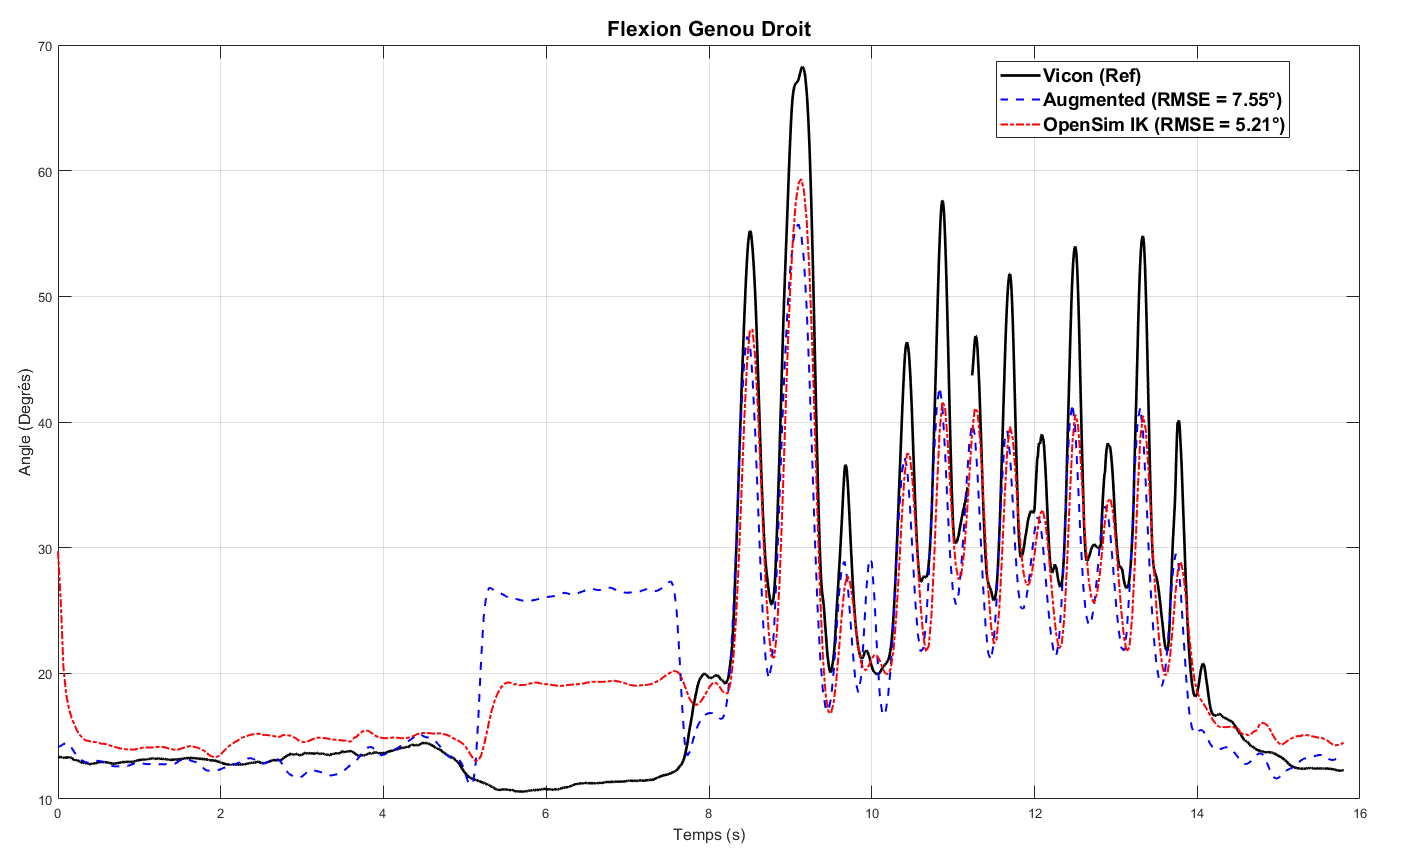
\includegraphics[width=\textwidth]{assets/Capture d'écran process/OpenSim/result.png}
        \caption{Comparaison des angles du genou droit avant et après l'IK d'OpenSim}
        \label{fig:ik_results}
    \end{figure}

    Pour clôturer cette partie, il a été observé que l'ajout des dernières étapes ont permis d'améliorer significativement la qualité des données biomécaniques obtenues avec le système MoCapIA en forçant un squelette humain cohérent sur les données. La $RMSE$ angulaire au début du stage était proche de celle obtenue avec OpenSim mais maintenant la longueur des membres est fixé et donc bien plus cohérente. De plus on dispose désormais de 43 marqueurs au lieu de 26, ce qui permet une analyse plus poussée des mouvements complexes.

\section{Recherche complémentaire : SAM 3D}

Durant le stage, une nouvelle méthode de capture de mouvement markerless a été publiée par Meta AI Research. Appelé \textbf{SAM 3D}, son fonctionnement est bien différent de MoCapIA. Cette technologie est capable de créer un modèle 3D avec seulement une image, un seul point de vue. Autrement dit, la multi-view n'est plus nécessaire ce qui pourrait mener à un gain de temps, de coût et de complexité phénoménal. Sorti en fin novembre 2025, elle pourrait bien révolutionner le domaine de la motion capture sans marqueur. Elle est composée de deux modèles distincts : SAM 3D Object pour les objets et scènes, \textbf{SAM 3D Body} pour les corps humains. C'est ce dernier qui va nous intéresser. Pour déduire une reconstruction 3D à partir d'une seule image, l'Intelligence Artificielle est au cœur de son fonctionnement :
\begin{figure}[H]
    \centering
    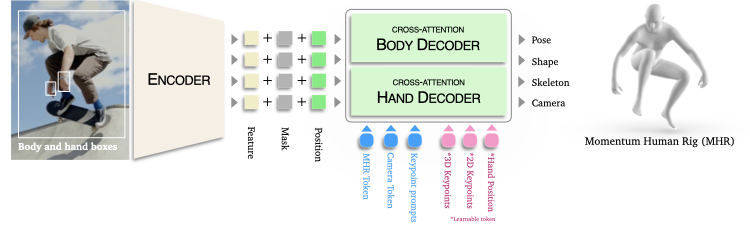
\includegraphics[width=0.8\textwidth]{assets/Capture d'écran process/SAM 3D/SAM3D_workflow.png}
    \caption{Processus SAM 3D Body}
    \label{fig:sam3D_workflow}
\end{figure}

Étant donné que cette technologie est toute récente, peu d'informations sont disponibles sur son fonctionnement interne. De plus, il n'existe pas encore de publication scientifique détaillant ses performances lors de tests rigoureux. Enfin son application est encore limitée à une image. Tel qu'il a été publié, il permet de retourner un modèle 3D à parti d'une image, mais pour l'instant incapable de créer un mouvement au cours du temps en 3D. Ce sont sur ces points que l'équipe a décidé d'approfondir ses recherches durant les dernières semaines du stage.

Disponible en opensource sur GitHub et HuggingFace, le code a été installé localement. En modifiant son code source, il a été possible de lui faire traiter des vidéos. En extrayant chaque frame de la vidéo, on peut ainsi obtenir une séquence de modèles 3D au cours du temps. Pour ça on exécute SAM 3D Body sur chaque frame de la vidéo. Il détecte de la même façon que MoCapIA les points caractéristiques 2D du corps humain à l'aide du modèle Halpe26. Il est donc à première vue possible de comparer ses performances à celle du Vicon et MoCapIA. Pourtant, des problèmes majeurs sont apparus lors de l'utilisation de SAM 3D Body :
\begin{itemize}
    \item Problème de référentiel : À chaque image, le modèle SAM 3D Body est lancé indépendamment. Même si le modèle 3D est centré sur le corps humain, on ne sait pas exactement comment il calcule le référentiel. En conséquence, le modèle 3D se décale dans l'espace au cours du temps.
    \item Problème d'échelle : Le modèle 3D retourné par SAM 3D Body n'est pas à l'échelle réelle. En effet, avec un seul point de vue, il estime la taille du sujet, mais sans aucune référence de distance. Le modèle, même si les coordonnées semblent justes, n'est pas à l'échelle réelle.
    
    \begin{figure}[H]
    \centering

    \begin{subfigure}{0.38
        \textwidth}
        \centering
        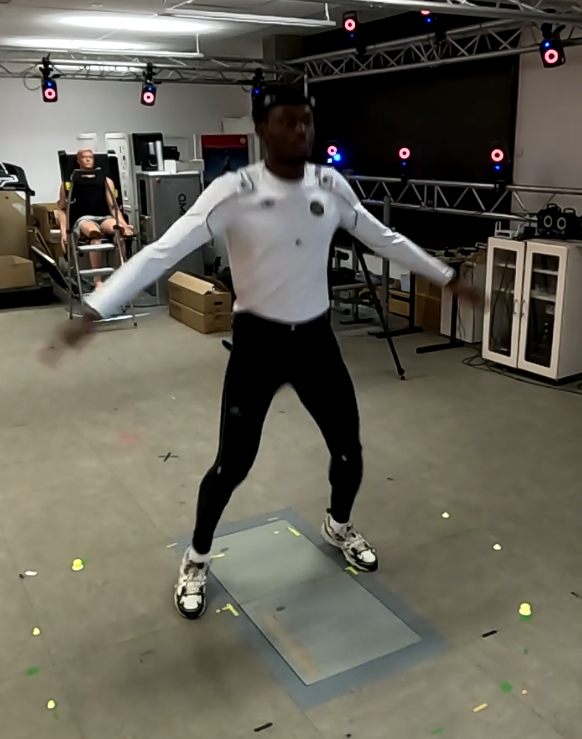
\includegraphics[width=\linewidth]{assets/Capture d'écran process/SAM 3D/sujet_SAM3D.png}
        \caption{Sujet capturé de 1,86 m}
        \label{fig:sam3d_subject}
    \end{subfigure}
    \hfill
    \begin{subfigure}{0.60\textwidth}
        \centering
        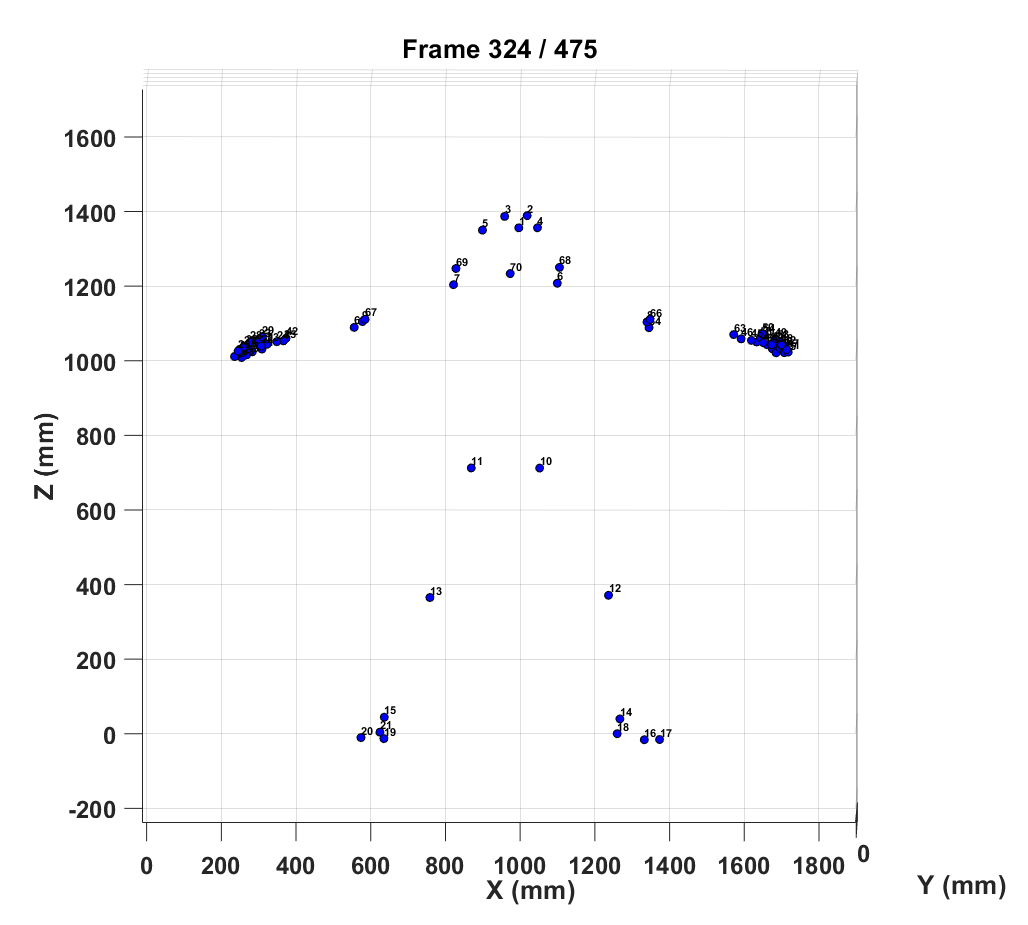
\includegraphics[width=\linewidth]{assets/Capture d'écran process/SAM 3D/modelSAM3D_2.png}
        \caption{Modèle 3D SAM 3D Body à la mauvaise échelle}
        \label{fig:sam3d_model}
    \end{subfigure}
    
    \caption{Problème d'échelle avec SAM 3D Body}
    \label{fig:SAM3D_scaleissues}
    \end{figure}
\end{itemize}

Des solutions auraient pu être développées pour corriger ces problèmes, mais avec le manque de temps, il a été décidé de s'arrêter à l'analyse angulaire des données 3D obtenues qui restent possibles malgré les problèmes cités précédemment. De la même façon que dans la partie \ref{estimation2D}, les angles articulaires ont été calculés et comparés aux données Vicon. L'objectif est maintenant de comparer les deux solutions - MoCapIA et SAM3D - à la méthode de référence Vicon afin d'identifier sur la méthode la plus performante. Les résultats montrent une erreur RMSE de $4.22^\circ$ pour le coude gauche et de $2.81^\circ$ pour le genou gauche soit des résultats équivalents à ceux de MoCapIA ($5.28^\circ$ et $2.74^\circ$ respectivement).

\begin{figure}[H]
    \centering
    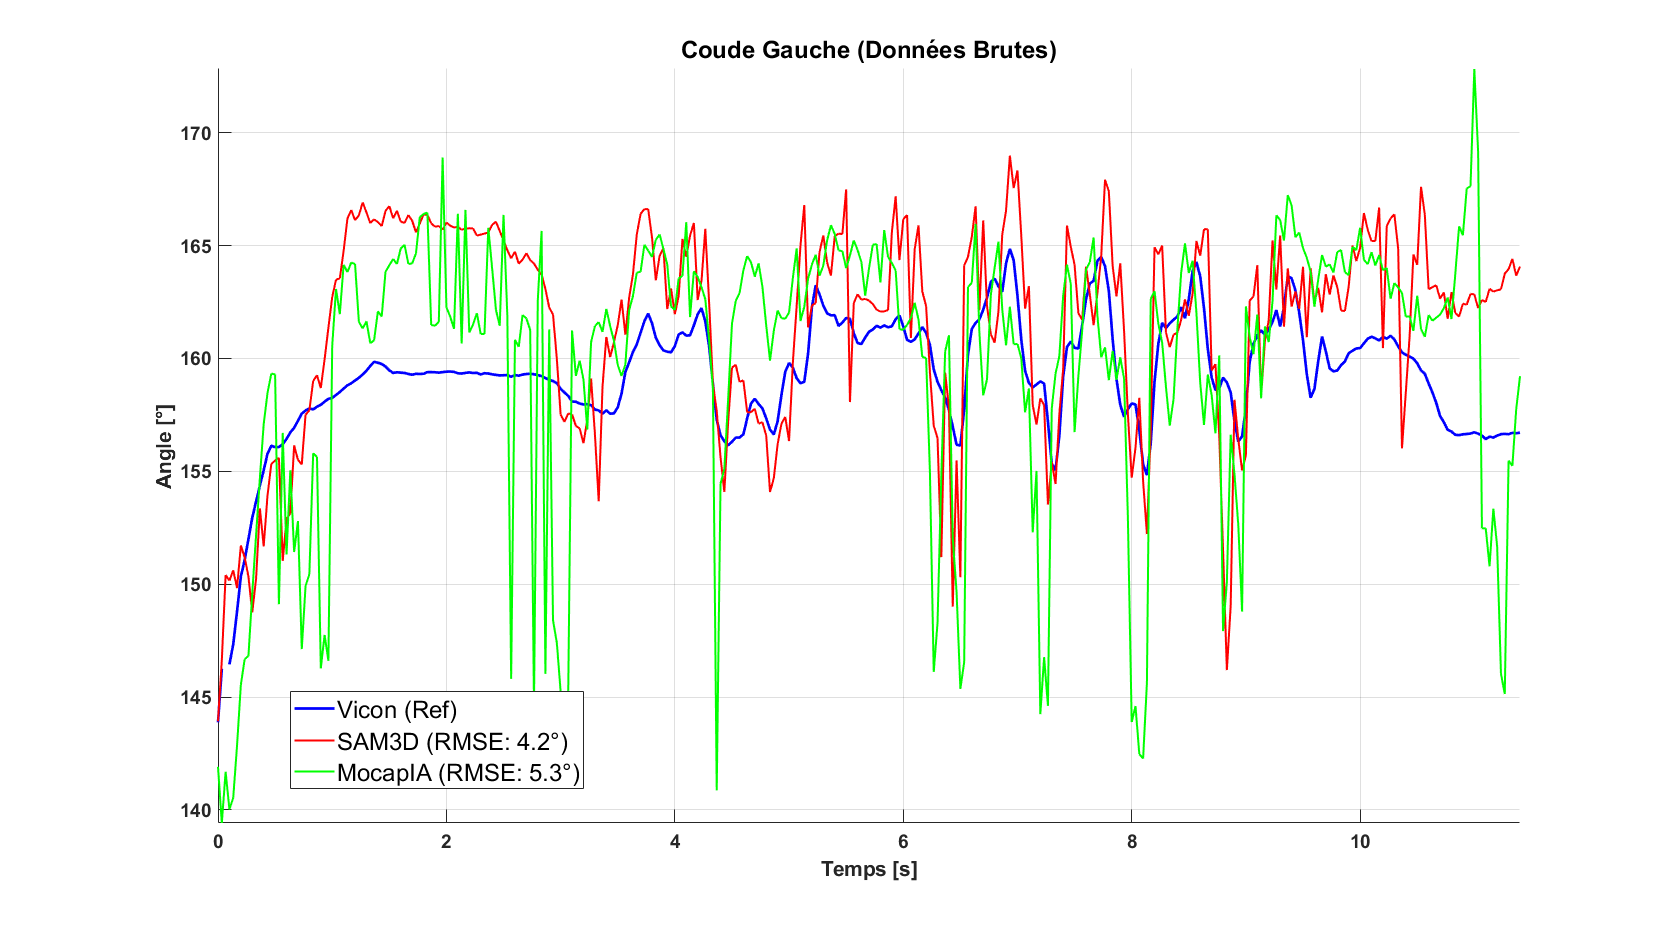
\includegraphics[width=\textwidth]{assets/Capture d'écran process/Vicon vs SAM3D vs MoCapIA/coudeG_vicon_sam3d_mocap.png}
    \caption{Comparaison à l'aide de la RMSE de l'angle du coude gauche entre Vicon, SAM 3D Body et MoCapIA}
    \label{fig:angle_coudeG_Vicon_SAM3D_MoCapIA}
\end{figure}

\begin{figure}[H]
    \centering
    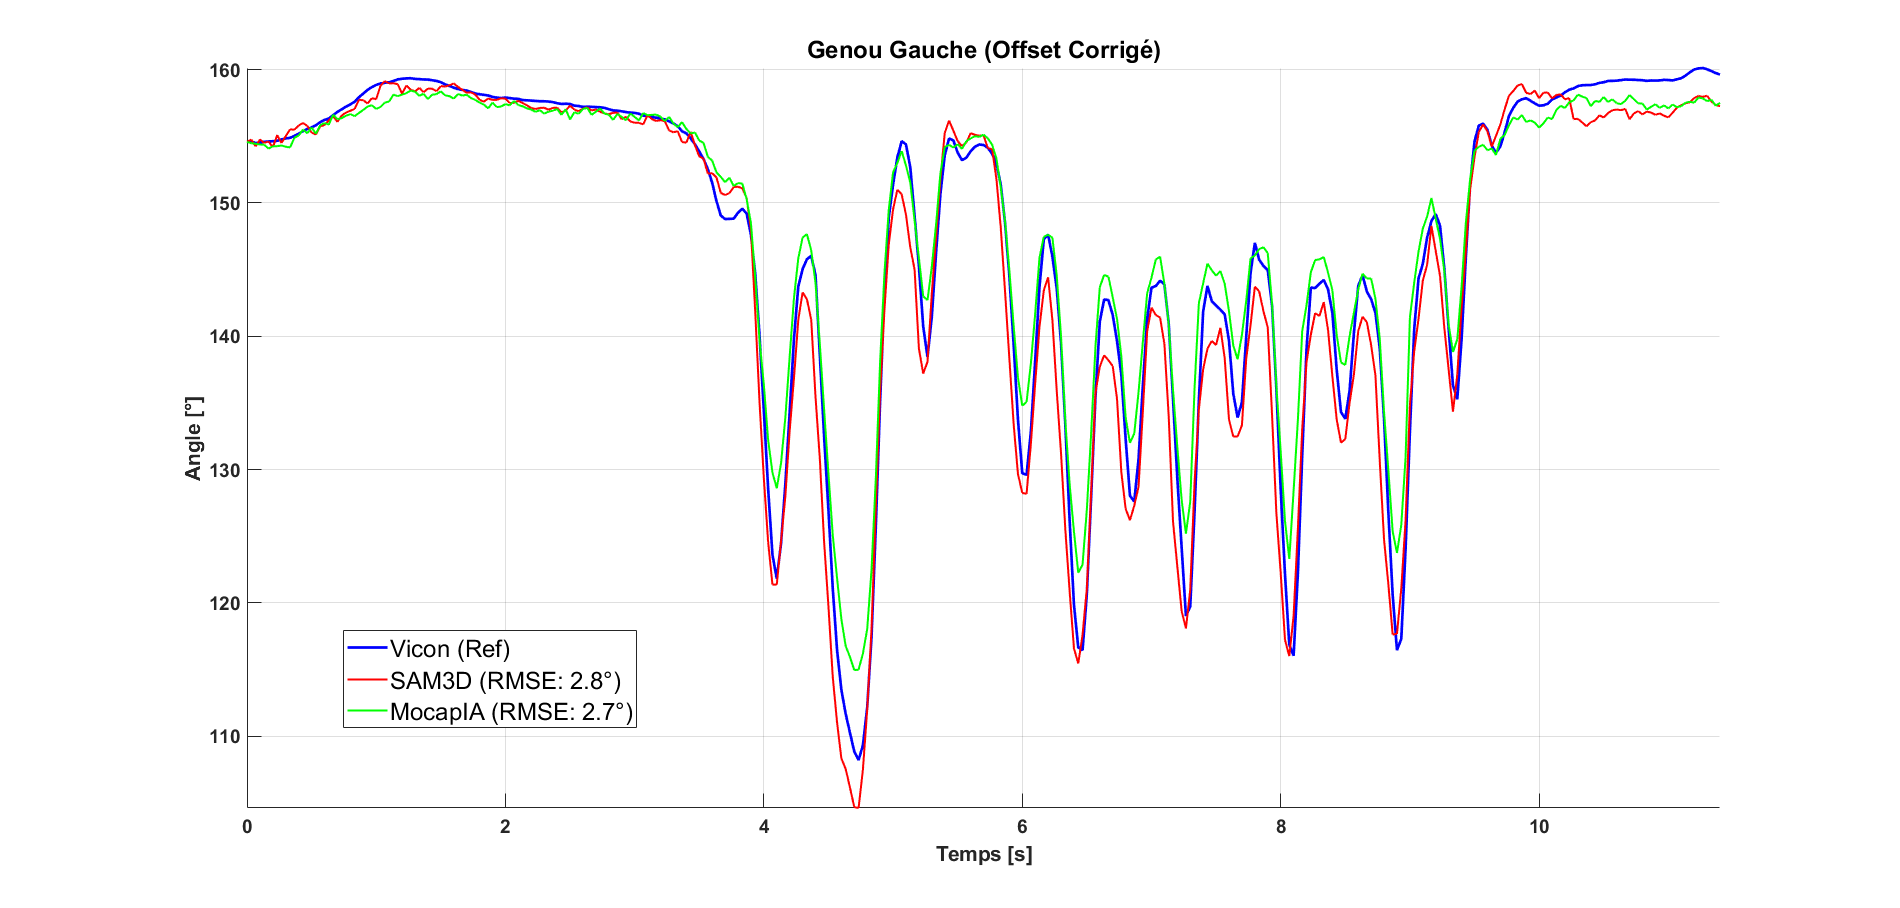
\includegraphics[width=\textwidth]{assets/Capture d'écran process/Vicon vs SAM3D vs MoCapIA/genouxG_vicon_sam3d_mocap.png}
    \caption{Comparaison à l'aide de la RMSE de l'angle du genou gauche entre Vicon, SAM 3D Body et MoCapIA}
    \label{fig:angle_genouG_Vicon_SAM3D_MoCapIA}
\end{figure}

Enfin une analyse de Bland-Altman a été réalisée pour valider ces résultats. Ils confirment ce qui vient d'être observé. En effet, pour le genou gauche (les autres articulations sont à retrouver en Annexe \ref{AnnexBlandAltmanSAM3D}), on observe que SAM 3D Body obtient des résultats similaires à MoCapIA avec un biais (une erreur systématique surement due au placement des marqueurs) de $-1.52^\circ$ et une variation aléatoire de $2.38^\circ$ contre un biais de $-0.97^\circ$ et une variation aléatoire de $2.54^\circ$ pour MoCapIA.

\begin{figure}[H]
    \centering
    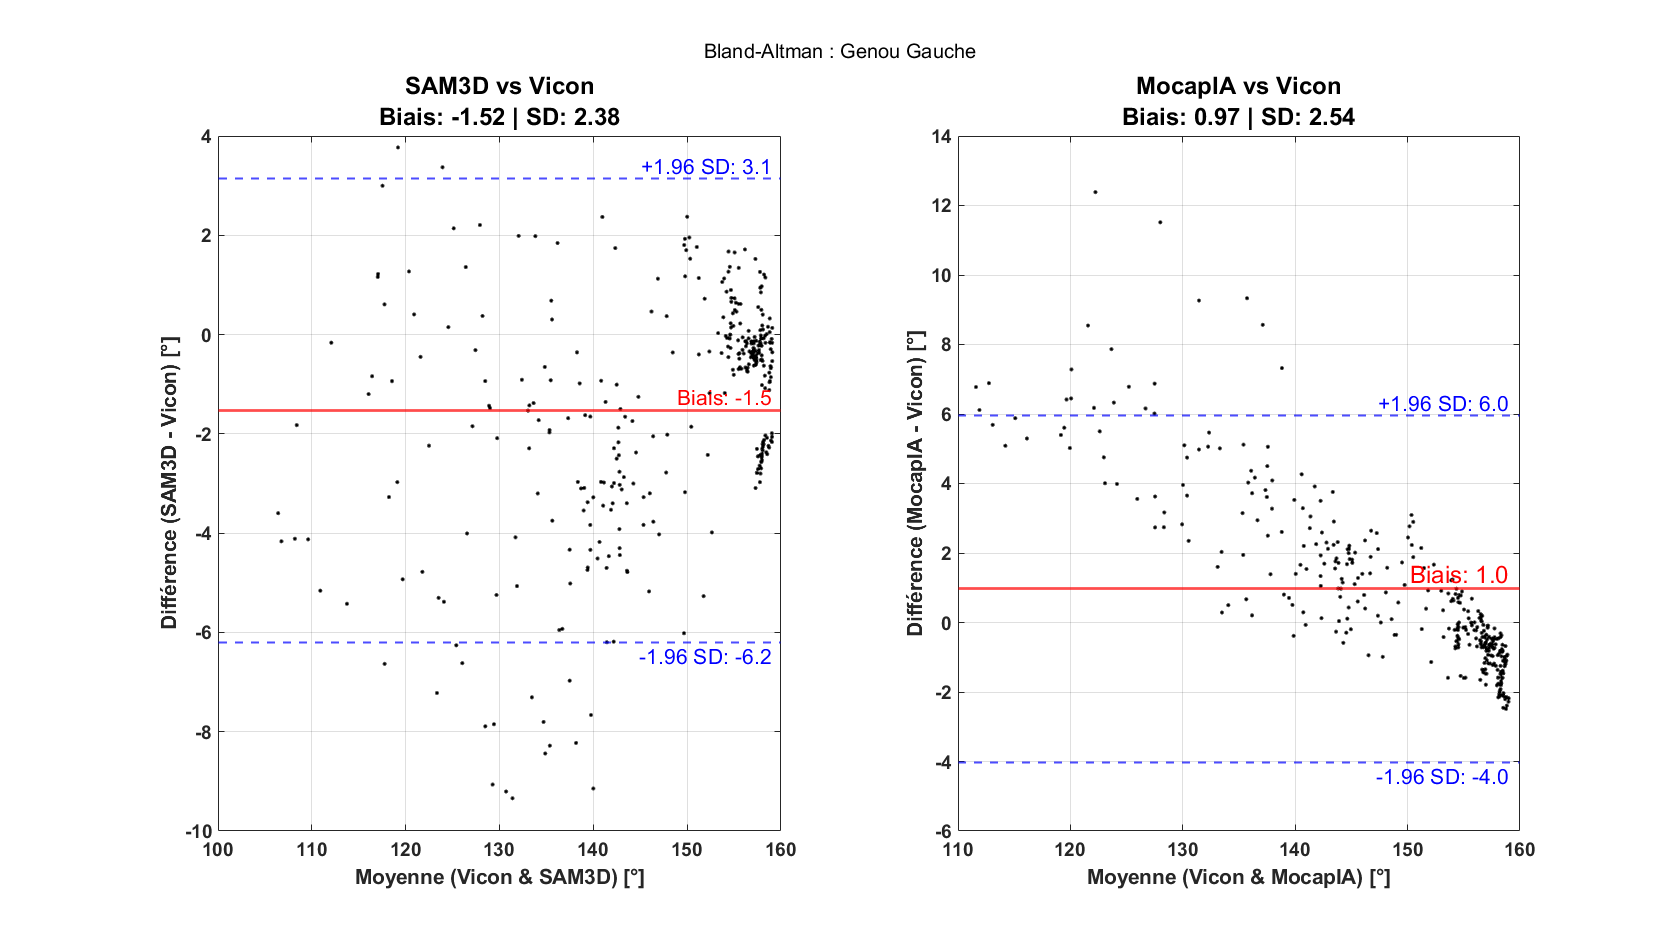
\includegraphics[width=\textwidth]{assets/Capture d'écran process/Vicon vs SAM3D vs MoCapIA/BlandAltman_Vicon_Mocap_sam3D.png}
    \caption{Analyse Bland-Altman entre Vicon, SAM 3D Body et MoCapIA pour le genou gauche}
    \label{fig:bland_altman_vicon_sam3d_mocapia}
\end{figure}

Même si les résultats sont légèrement meilleurs que MoCapIA, il est important de noter que les positions des points 3D de Sam 3D Body n'ont pas pu être comparées directement aux données Vicon et MoCapIA à cause des problèmes de référentiel et d'échelle. Ainsi, l'analyse angulaire seule ne permet pas de conclure définitivement sur la supériorité de SAM 3D Body par rapport à MoCapIA. Toutefois, ces résultats restent prometteurs pour une technologie aussi récente et pourraient faire partie des futures perspectives à donner au projet MoCapIA. 
    \chapter{Conclusion}

\section{Résumé du Stage}
    
    Dans ce rapport, les principales activités et réalisations effectuées durant mon stage ont été présentées. Ces travaux visaient à améliorer le processus MoCapIA, allant de la calibration jusqu'à la reconstruction 3D d'un modèle humain en passant par l'estimation 2D sans marqueurs et la triangulation des données pour des applications cliniques, sportive ou industrielle. Quatre anciens stagiaires avaient auparavant travaillé sur le projet. Ils ont développé la majorité des fonctions de base du processus et testé les différentes technologies à dispositions (ex : modèle d'estimateur de pose 2D) tout en respectant les conventions de programmations.
    
    Il a donc été facile durant la première phase, de comprendre le code existant et se familiariser avec l'Interface Utilisateur. Avec l'aide du précédent stagiaire et de mon tuteur de stage, une démo a été réalisée en début de stage ce qui m'a permis d'observer les différentes étapes et surtout d'identifier les points faibles du projet MoCapIA. Par la suite, mon tuteur de stage m'a incité à conduire une veille scientifique en se reposant sur une recherche bibliographique approfondie dans les domaines de la capture de mouvement et de l'estimation de pose afin d'identifier les avancées récentes. J'ai rapidement compris que cette étape était essentielle pour comprendre les enjeux, mais notamment pour identifier les éventuelles améliorations.
    
    Dans un deuxième temps, l'objectif était d'identifier les points faibles du processus sur la base de mesures expérimentales. Pour ça, on a mis en place une série d'expériences :
    \begin{itemize}
        \item \textbf{TEST 0} afin de comprendre l'impact du damier sur la qualité de la calibration.
        \item \textbf{TEST 1} sur l'homogénéisation de la calibration en mettant de côtés les erreurs d'estimation 2D.
        \item \textbf{TEST 2} a permis de comparer RTMPose, l'estimateur de pose 2D utilisé dans MoCapIA, avec une méthode de référence avec marqueur (Vicon).
    \end{itemize}
    Ces différents tests nous ont permis de conclure que l'estimation 2D des points caractéristiques était le maillon faible. 
    
    Dans un troisième temps, une importante étape de recherche bibliographique a été réalisée afin de remédier aux problèmes mis en lumière ci-dessus. J'ai donc implémenté de nouvelles méthodes pour affiner et corriger les points 2D détectés. En s'inspirant d'un projet similaire (Pose2Sim) qu'on a d'abord comparé avec MoCapIA, 3 étapes ont été retenues et adaptées à notre processus. Le filtrage a permis de supprimer les valeurs incohérentes et de supprimer le bruit lié aux erreurs d'estimation 2D. Les deux autres étapes ont permis, en plus de figer la distance des membres en appliquant un squelette au modèle 3D,d'augmenter le nombre de marqueurs afin de permettre une analyse biomécanique bien plus complète. Chaque étape a été testée et validée individuellement avant d'être intégrée dans le processus global. Des tests finaux ont été réalisés pour valider l'ensemble des améliorations apportées. Les résultats ont montré une nette amélioration de la qualité de la reconstruction 3D, confirmant l'efficacité des nouvelles étapes implémentées. 
    
    Enfin, grâce à une veille technologique, nous avons pu tester un nouvel outil de capture 3D de mouvement basée uniquement sur une caméra et l'IA SAM3D de Meta. En effet, même si son application sur une vidéo reste pour l'instant complexe, SAM3D a ouvert une nouvelle voie dans le domaine de la capture de mouvement avec des résultats très prometteurs. Il est possible de modéliser le mouvement d'un être humain en 3D avec seulement une caméra et sans avoir besoin de calibration, on se rapproche encore plus des objectifs de moindres coûts et de simplicité. Entre temps, j'ai ajouté des fonctionnalités secondaires au logiciel ; pour permettre de gérer quelques paramètres comme la possibilité de choisir précisément quelles parties lancées (ex : pouvoir choisir quel filtre appliqué avec quels paramètres) qui n'a pas pu être ajouté dans l'interface utilisateur. Les étapes principales ajoutées, elles, ont par ailleurs été intégrées dans l'interface grâce à la deuxième stagiaire Yiyang.

\section{Analyse réflexive}
    
    \paragraph{Analyse Critique}

        Cette partie va permettre d'effectuer une conclusion critique et personnelle sur le travail accompli et ces six mois passé au BMBI, en soulignant ce qui a fonctionné et ce qui ne l'a pas été. Je vais aussi explorer les points positifs et négatifs de cette mission. Enfin, je vais mettre en lumière les compétences que j'ai pu développer durant ce stage et leur cohérence ou non avec mon projet professionnel.

        Premièrement le sujet du stage m'a beaucoup plu. En effet, la capture de mouvement est un domaine qui m'intéresse depuis longtemps, j'avais d'ailleurs effectué un projet de fin de cursus en classe préparatoire sur le thème de la capture de trajectoire de balle. Ce projet reprenait en grande partie les notions de calibration et de triangulation, mais aussi de traitement d'images et de détection par une IA qu'on a utilisé dans le projet MoCapIA. J'ai donc pu approfondir mes connaissances dans ces domaines et découvrir de nouvelles notions comme la dimension biomécanique et les technologies d'estimations de pose humaine.

        Deuxièmement, la dimension "recherche" du stage a été vraiment une bonne expérience. Cela m'a permis de me familiariser avec la recherche bibliographique scientifique en anglais et de comprendre l'importance de cette étape dans le développement d'un projet innovant. Je pense avoir acquis une bonne méthodologie de recherche documentaire qui me sera utile dans le futur. Que ce soit dans le domaine de la recherche ou de l'entreprise, la rigueur et la nécessité de valider l'ensemble de ses choix par des sources fiables est, à mon sens, un point essentiel.

        Troisièmement, ce stage a été effectué à deux. En effet, avec Yiyang Huang, une étudiante GI04, elle aussi en TN09, nous avons partagé le même tuteur de stage et avons travaillé sur le même projet MoCapIA. Cela a impliqué la mise en place d'une coordination et d'une collaboration efficace pour la réalisation des tâches, ce qui au final a été l'un des points positifs du stage. En effet, ce travail collaboratif pour la conception d'un logiciel et les tests menés avec le groupe de TX a permis d'introduire à plus grande échelle la notion de travail en équipe sur quelque chose de concret. Nous avons utilisé des outils de gestion de version (Git / GitLab pour le stockage) et de communication (réunions hebdomadaires). Le fait d'avoir une autre personne avec qui échanger sur les problématiques rencontrées est aussi un point vraiment important. 
        
        Les réalisations qui ont été exposés dans ce rapport ont permis d'atteindre les objectifs fixés au début du stage. Les étapes de test ont été concluantes et m'ont servis tout au long du stage pour orienter mes recherches. On peut toutefois critiquer certains aspects des expériences. En effet, lors du \textbf{TEST 1 - Analyse de l'homogénéisation de la calibration}, on triangule quand même les résultats pour calculer l'erreur de calibration. Lors des clics effectués pendant l'expérience, on obtient toujours une erreur de quelques pixels ce qui implique une légère approximation quand on applique l'algorithme de triangulation. Une étude de sensibilité pourrait compléter l'analyse. En affirmant que l'on mesure uniquement l'erreur de calibration, on néglige cette erreur de triangulation et on émet l'hypothèse qu'elle reste négligeable par rapport à l'erreur de calibration. Cependant, cette erreur est très faible comparée à l'erreur de calibration, on considère donc cette hypothèse comme acceptable. Je rajouterai que lors du test entre le système optoélectronique Vicon et le système MoCapIA, on considère le Vicon comme la référence absolue. Il est pourtant important de noter que ce système souffre aussi d'erreurs, notamment en provenance des approximations humaines lors du placement de marqueurs. Les erreurs observées lors de la conclusion sont donc à nuancer \cite{MarkerlessforBiomecha}. On peut aussi nuancer la conclusion de la comparaison entre MoCapIA et SAM3D. En effet, la comparaison de SAM a été faite avec la version de MoCapIA sans les corrections biomécaniques.

        Des difficultés ont été rencontrées durant le stage. La plus importante a été la recherche bibliographique. En effet, c'était quelque chose d'assez nouveau. Au début, j'étais incapable de cibler les bonnes informations dans les articles et j'utilisais des assistants conversationnels pour m'aider à résumer les articles. Cette approche n'était pas la bonne, mais au fur et à mesure, j'ai pu m'améliorer et apprendre à extraire les informations importantes par moi-même. Mon tuteur de stage m'a aussi beaucoup aidé en me guidant dans mes recherches et en me donnant des pistes à explorer tout au long du stage. Une autre difficulté rencontrée a été la compréhension du code. En effet, étant un projet de stage depuis deux ans, le logiciel contenait plusieurs dizaines de fichiers et plusieurs milliers de lignes de code. Même si les conventions de programmations étaient respectées, il a fallu un certain temps pour se familiariser avec l'architecture du code et le dialogue entre les différentes fonctions et l'interface utilisateur.

        Finalement ce stage m'a permis de développer plusieurs compétences et d'affiner mon projet professionnel. En matière d'intelligence artificielle, j'ai pu approfondir mes connaissances sur les modèles de deep learning, avec l'utilisation des bibliothèques PyTorch et Tensorflow.
        J'ai pu renforcer mes compétences en traitement d'images et en vision par ordinateur, notamment à travers les étapes de calibration, d'estimation de pose 2D et de la reconstruction 3D. J'ai pu m'initier à la programmation orientée objet en Python (habitué au C++) en travaillant sur ce projet 100\% codé en python. Le concept est le même, mais j'ai pu remarquer plusieurs différences, car Python est plus souple que le C++. Pour ce qui est des algorithmes de traitement de résultats, surtout pour des tests statistiques et graphiques, j'ai majoritairement utilisé MATLAB, ce qui me permet aujourd'hui d'être encore plus à l'aise avec ce langage. L'aspect mathématique du projet m'a beaucoup plu, particulièrement avec les notions de géométrie projective et d'algèbre linéaire. L'équipe BioMov-E accueille plusieurs doctorants et chercheurs internationaux donc chaque réunion hebdomadaire se déroulait en anglais ; cela m'a permis d'améliorer mon niveau d'anglais scientifique. 
        Je n'exclus pas la possibilité de poursuivre dans la recherche, même si je compte orienter ma recherche de stage TN10 en entreprise. Je pense m'orienter vers la filière INES pour la suite de mon cursus, car j'ai apprécié la vision par ordinateur et j'aimerais l'appliquer à la robotique ou à des systèmes autonomes.


    \paragraph{Impact sociétal / éthique}

        Ce projet s'inscrit dans un contexte dans lequel la technologie se retrouve au service de la santé. Il a pour but d'améliorer les diagnostics des professionnels de santé en leur fournissant des outils plus précis sans pour autant augmenter considérablement les coûts. En rendant la capture de mouvement plus accessible, on permet à un plus grand nombre de patients de bénéficier d'analyses détaillées de leurs mouvements. Utilisant des modèles d'intelligence d'artificielle, l'utilisation de cette technologie pourrait inquiéter le patient sur les données recueillies et utilisées. Pourtant, ces données se réduisent pour l'instant à des informations de base comme la taille, le poids, l'âge et le sexe ; cela reste donc relativement peu intrusif. De plus, le logiciel est aussi destiné aux sportifs de hauts niveaux ou aux entraîneurs, leur permettant d'analyser les performances et de prévenir les blessures grâce à une analyse biomécanique détaillée.

        Le projet a donc plusieurs intérêts sociétaux. Les impacts environnementaux sont, eux aussi, limités. En effet, en utilisant des caméras classiques et en réduisant le nombre de capteurs nécessaires, on diminue la consommation de ressources matérielles. Même si beaucoup d'énergie ont été nécessaires pour entraîner les modèles d'IA que l'on utilise, l'impact sur la durée totale de vie reste vraiment faible.

    \paragraph{Perspectives}

        L'écriture de ce rapport a permis de faire le point sur les différentes étapes du projet et d'identifier des pistes d'améliorations futures. Plusieurs axes de développement peuvent être envisagés pour continuer à améliorer le processus MoCapIA. En suivant de près les avancées dans le domaine de l'IA, on pourrait intégrer de nouveaux modèles d'estimation de pose 2D encore plus performants. Même si RTMPose reste le modèle le plus adapté à la fin de ce stage, de nouvelles technologies font leur apparition. C'est le cas pour le modèle SAM3D qui a montré des résultats prometteurs. Si la prochaine équipe réussie à comprendre plus en détails cette technologie et réussi à l'adapter à des vidéos complètes, on pourrait répondre encore mieux aux objectifs initiaux du projet MoCapIA.
        L'interface utilisateur pourrait aussi être amélioré en intégrant plus de paramètres de contrôle pour les différentes étapes du processus et en s'inspirant des logiciels de santé et de gestion de patient.
        Une façon plus simple de calibrer avec les caméras pourrait être implémentée. Avec une disposition de caméras aux quatre angles de la zone de capture, la calibration avec un damier devient compliquée. L'utilisation d'objets de calibration en trois dimensions pourraient simplifier cette étape \cite{OtherCalibMethods}.

    
    % Bibliographie
    \printbibliography[heading=bibintoc]
    \chapter*{Glossaire} % Le * évite de numéroter "Chapitre X"
\addcontentsline{toc}{chapter}{Glossaire} % Ajoute manuellement au sommaire
\markboth{Glossaire}{Glossaire} % Corrige l'en-tête de page

% Début de la liste de définitions
\begin{description}
    \setlength{\itemsep}{1em} % Ajoute de l'espace entre les définitions pour aérer

    \item[\textbf{\underline{Binning}}] 
    Technique de regroupement de données en "bins" (ou boîtes) pour réduire le bruit.

    \item[\textbf{\underline{BioMov-E}}] 
    Équipe de recherche du labo BMBI spécialisée dans la BioMécanique et le mouvement humain.

    \item[\textbf{\underline{Bland-Altman}}] 
    Méthode statistique utilisée pour comparer deux techniques de mesure.

    \item[\textbf{\underline{BMBI}}] 
    BioMécanique et BioIngénierie, laboratoire de recherche de l'UTC où le stage a été effectué.

    \item[\textbf{\underline{Bounding box}}] 
    Boîte englobante, un rectangle délimitant une région d'intérêt dans une image, souvent utilisé en vision par ordinateur pour localiser des objets/personnes.

    \item[\textbf{\underline{Calibration}}] 
    Processus permettant de déterminer la position et l'orientation des caméras dans l'espace 3D ainsi que leurs paramètres intrinsèques (focale, distorsion).

    \item[\textbf{\underline{Cinématique Inversée}}] 
    Méthode utilisée en robotique et en animation pour déterminer les angles des articulations nécessaires afin d'atteindre une position ou une orientation spécifique d'un segment ou d'un effecteur.

    \item[\textbf{\underline{CNRS}}] 
    Centre National de la Recherche Scientifique.

    \item[\textbf{\underline{Complexité computationnelle}}] 
    Mesure de la quantité de ressources nécessaires pour exécuter un algorithme, souvent en nombre d'opérations ou d'espace mémoire.

    \item[\textbf{\underline{Distorsion}}] 
    Déformation optique des images capturées par les caméras.

    \item[\textbf{\underline{Écart type}}] 
    Mesure statistique de la dispersion des valeurs autour de la moyenne.

    \item[\textbf{\underline{Estimation 2D}}] 
    Processus d'identification des positions des points d'intérêt dans une image 2D, souvent utilisé en vision par ordinateur est effectué par RTMPose dans MoCapIA.

    \item[\textbf{\underline{Filtre Butterworth}}] 
    Type de filtre de traitement du signal conçu pour offrir une réponse en fréquence la plus plate possible dans la bande passante (sans ondulations), tout en atténuant progressivement les fréquences indésirables au-delà d'une certaine limite appelée fréquence de coupure.

    \item[\textbf{\underline{Filtre Butterworth Speed}}] 
    Type de filtre de traitement du signal qui privilégie la réduction du déphasage et du temps de réponse pour traiter des signaux en temps réel sans retard excessif.

    \item[\textbf{\underline{Filtre Gaussian}}] 
    Technique de lissage qui réduit le bruit d'une image ou d'un signal en calculant pour chaque point une moyenne pondérée de ses voisins, où les poids sont définis par une courbe en cloche (la fonction de Gauss) afin d'accorder une importance maximale au centre et de l'atténuer progressivement avec la distance.

    \item[\textbf{\underline{Filtre GCV Spline}}] 
    Méthode d'ajustement de courbe qui utilise une fonction mathématique flexible (spline) dont le degré de lissage est automatiquement optimisé en cherchant à minimiser l'erreur de prédiction globale sans nécessiter de connaître à l'avance le niveau de bruit des données.

    \item[\textbf{\underline{Filtre Hampel}}] 
    Algorithme robuste qui détecte et remplace les valeurs aberrantes (outliers) dans une série temporelle en analysant chaque point au sein d'une fenêtre mobile.

    \item[\textbf{\underline{Filtre Kalman}}] 
    Algorithme récursif qui estime l'état d'un système dynamique (comme la position d'un avion ou d'une voiture) en fusionnant des prédictions théoriques incertaines avec des mesures réelles bruitées, afin de produire l'estimation la plus précise possible en temps réel.

    \item[\textbf{\underline{Filtre LOESS}}] 
    Méthode de régression locale qui lisse une courbe en ajustant une multitude de modèles simples (généralement des polynômes de bas degré) sur de petites fenêtres de données glissantes, accordant plus de poids aux points les plus proches de la zone à estimer.

    \item[\textbf{\underline{Focale}}] 
    Distance entre le centre optique de la lentille et le capteur, déterminant le champ de vision de la caméra.

    \item[\textbf{\underline{Logs}}] 
    Fichiers journaux enregistrant les événements et les erreurs survenus lors de l'exécution du logiciel MoCapIA.

    \item[\textbf{\underline{Markerless}}] 
    En français "sans marqueurs", ce terme est utilisé pour désigner les systèmes de capture de mouvement qui n'utilisent pas de marqueurs physiques attachés au corps.

    \item[\textbf{\underline{mocap}}] 
    De l'anglais "motion capture", capture de mouvement en français.

    \item[\textbf{\underline{MoCapIA}}] 
    Projet sur lequel le stage porte – c'est un système de capture de mouvement sans marqueurs physiques.

    \item[\textbf{\underline{Multi-view}}] 
    Technique utilisant plusieurs points de vue ou caméras pour reconstruire une scène ou un objet en 3D.

    \item[\textbf{\underline{Offset}}] 
    Valeur de décalage constant sur l'ensemble du signal.

    \item[\textbf{\underline{OpenSim}}] 
    Package open-source de simulation musculo-squelettique utilisé pour l'analyse biomécanique développée dans le cadre du logiciel OpenSim.

    \item[\textbf{\underline{Pipeline}}] 
    Ensemble des étapes de traitement des données dans un processus.

    \item[\textbf{\underline{Plage de fonctionnement}}] 
    Intervalle dans lequel 95\% des données mesurées se situent.

    \item[\textbf{\underline{Pose2Sim}}] 
    Autre projet de capture de mouvement sans marqueurs.

    \item[\textbf{\underline{PyQt5}}] 
    Bibliothèque Python pour créer des interfaces graphiques, utilisée dans le projet MoCapIA.

    \item[\textbf{\underline{Scaling}}] 
    En français "mise à l'échelle", processus d'ajustement de l'échelle des données pour les rendre comparables ou pour améliorer la performance des algorithmes.

    \item[\textbf{\underline{Timecode}}] 
    Système de synchronisation temporelle entre plusieurs dispositifs d'enregistrement, ici les caméras.

    \item[\textbf{\underline{Triangulation}}] 
    Méthode utilisée pour déterminer la position 3D d'un point en utilisant plusieurs vues 2D provenant de caméras différentes.

    \item[\textbf{\underline{TSS}}] 
    Technologie Sport Santé, plateforme dédiée à l'analyse du mouvement humain au sein du laboratoire BMBI.

    \item[\textbf{\underline{Valeurs aberrantes}}] 
    Données qui s'écartent significativement des autres observations, pouvant indiquer une erreur ou une variabilité inhabituelle.

    \item[\textbf{\underline{Vicon}}] 
    Vicon T160 est un système de capture de mouvement optoélectronique de référence composé ici de 18 caméras MXT160, 12 caméras Bonita 3 ainsi que 7 caméras Vantage 5.

\end{description}
    
    %Liste des figures et des tableaux
    \listoffigures
    %\listoftables
    

    % Annexes
    %affichage dans sommaire sans numero
\chapter{Annexes}
\addcontentsline{toc}{chapter}{Annexes}


\section{Annexe 1 - Triangulation Global/Locale}
\label{AnnexTriangu}
    Dans cette annexe est présentée une expérience complémentaire sur la triangulation globale et locale. MoCapIA utilise la  \textbf{triangulation locale} pour reconstruire les positions 3D des marqueurs. Pour ça le système utilise les coordonnées 3D estimées à partir de chaque paire de caméras, utilise une méthode de \textit{binning} qui consiste à regrouper les points 3D proches dans des \textit{bins} (ou boîtes) de taille fixe, puis on effectue la moyenne du \textit{bins} le plus rempli pour obtenir la position 3D finale du marqueur.

    À première vue, même si on utilise la moyenne, on utilise pour obtenir la triangulation du point 3D seulement deux caméras. Une autre option existe : la \textbf{triangulation globale}. Cette méthode consiste à calculer dans un premier temps les coordonnées 3D à partir d'une paire de caméras, puis de re-projeter ces coordonnées 3D en 2D pour les comparer avec les paramètres 2D de toutes les autres caméras. Le point 3D est donc ajusté pour minimiser l'erreur de reprojection sur toutes les caméras. Cette méthode permet donc d'utiliser l'information de toutes les caméras pour chaque point 3D.

    Pourtant, cette méthode n'a pas été concluante dans le cadre de MoCapIA. En effet, en testant cette méthode sur les données de calibration, on obtient une erreur de reprojection plus importante (voir figure \ref{fig:triangulation_global_local}).
    \begin{figure}[H]
        \centering
        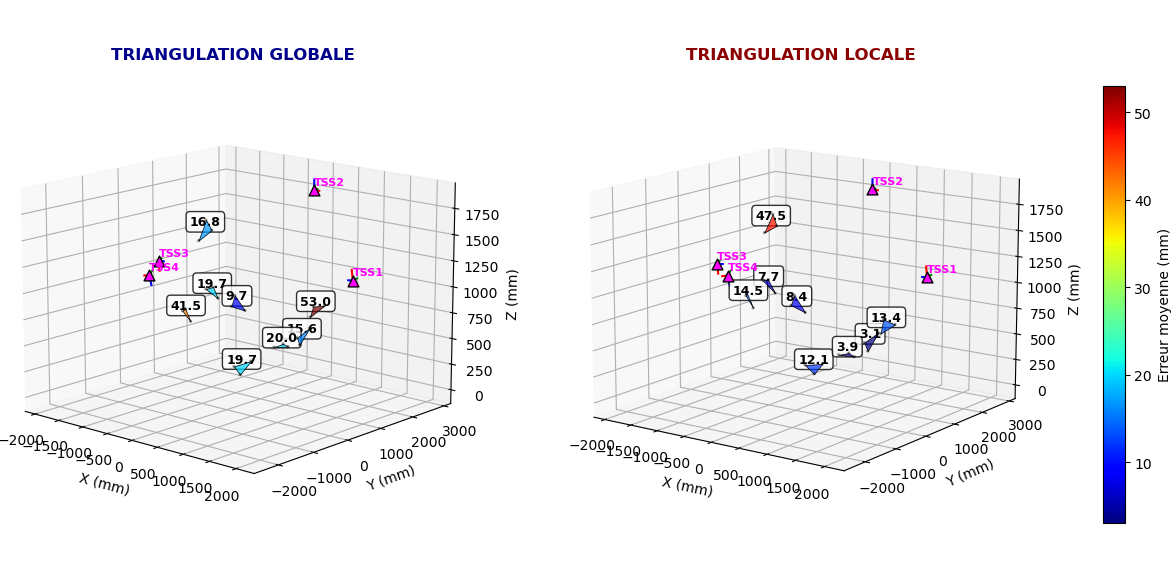
\includegraphics[width=\textwidth]{assets/Capture d'écran process/Précision_CalibTriangulation/triangulation_test.png}
        \caption{Comparaison de l'erreur de triangulation globale et locale}
        \label{fig:triangulation_global_local}
    \end{figure}
    La triangulation locale obtient une erreur moyenne de $13.83mm$ contre $24.50mm$ pour la triangulation globale. On a donc conservé la méthode de triangulation locale pour la suite du stage.

\section{Annexe 2 - Autres résultats de la comparaison Vicon - MoCapIA}
\label{AnnexVicon_Mocap}
    Dans cette annexe sont présentés les résultats complémentaires de la comparaison entre le système de référence Vicon et le système MoCapIA. 

    \begin{figure}[H]
        \centering
        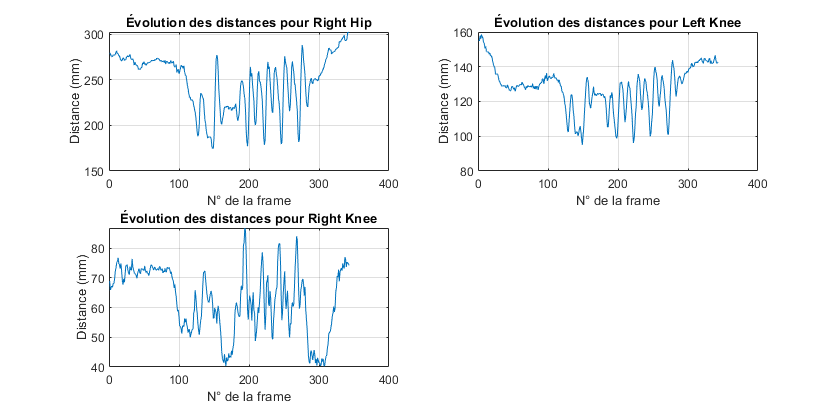
\includegraphics[width=\textwidth]{assets/Capture d'écran process/TX_ViconVSMocapIA/evolution_distance_Mocap.png}
        \caption{Évolution de la distance}
    \end{figure}
    \begin{figure}[H]
        \centering
        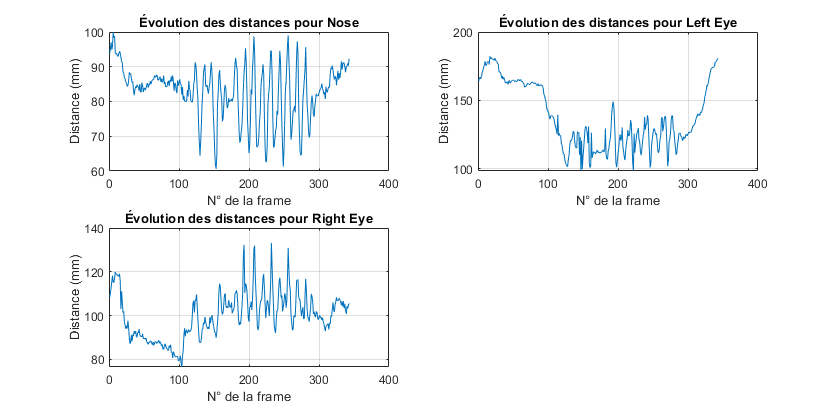
\includegraphics[width=\textwidth]{assets/Capture d'écran process/TX_ViconVSMocapIA/evolution_distance_Mocap11.png}
        \caption{Évolution de la distance}
    \end{figure}
    \begin{figure}[H]
        \centering
        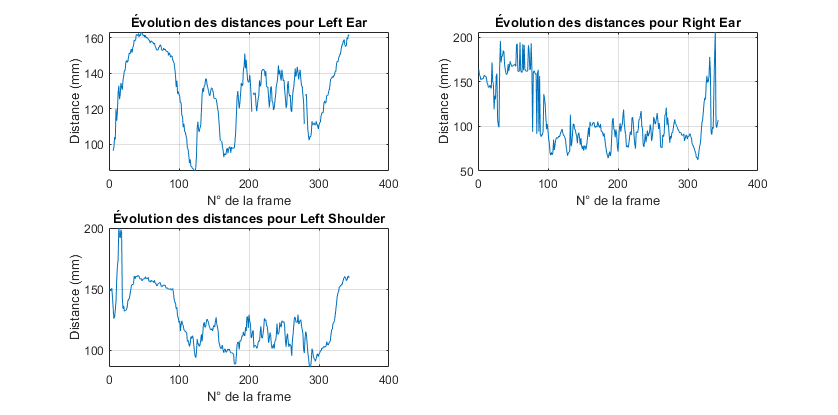
\includegraphics[width=\textwidth]{assets/Capture d'écran process/TX_ViconVSMocapIA/evolution_distance_Mocap12.png}
        \caption{Évolution de la distance}
    \end{figure}
    \begin{figure}[H]
        \centering
        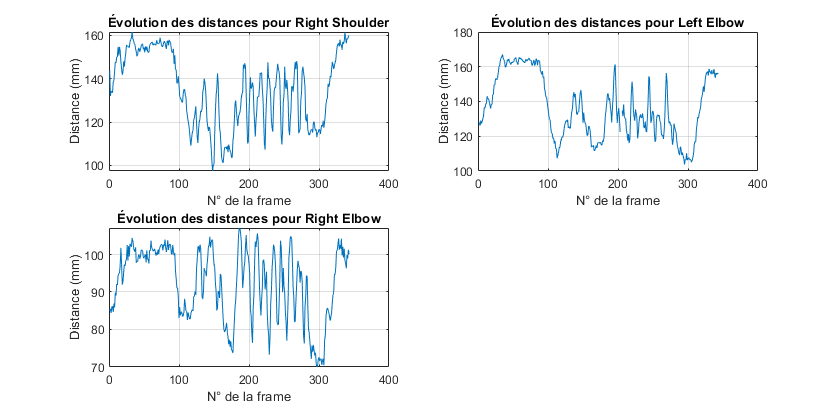
\includegraphics[width=\textwidth]{assets/Capture d'écran process/TX_ViconVSMocapIA/evolution_distance_Mocap13.png}
        \caption{Évolution de la distance}
    \end{figure}
    \begin{figure}[H]
        \centering
        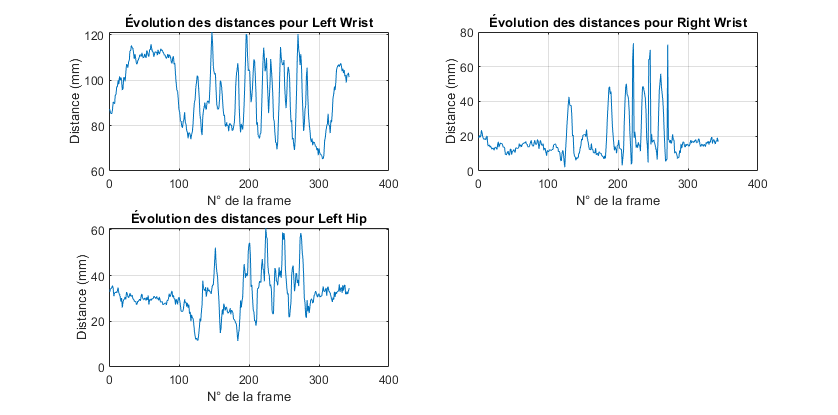
\includegraphics[width=\textwidth]{assets/Capture d'écran process/TX_ViconVSMocapIA/evolution_distance_Mocap14.png}
        \caption{Évolution de la distance}
    \end{figure}
    \begin{figure}[H]
        \centering
        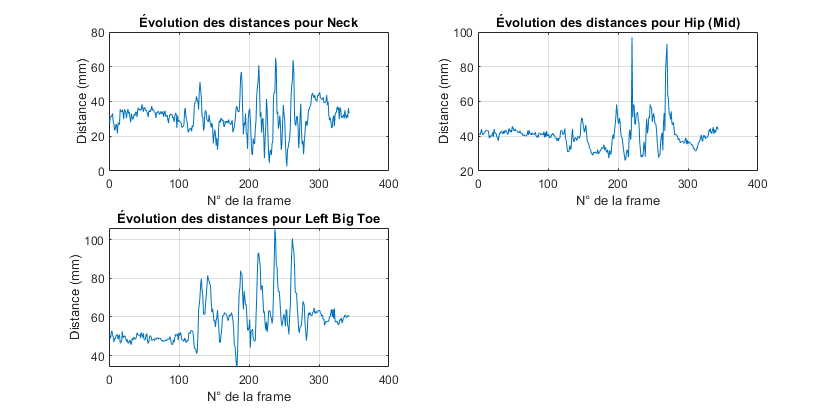
\includegraphics[width=\textwidth]{assets/Capture d'écran process/TX_ViconVSMocapIA/evolution_distance_Mocap17.png}
        \caption{Évolution de la distance}
    \end{figure}
    \begin{figure}[H]
        \centering
        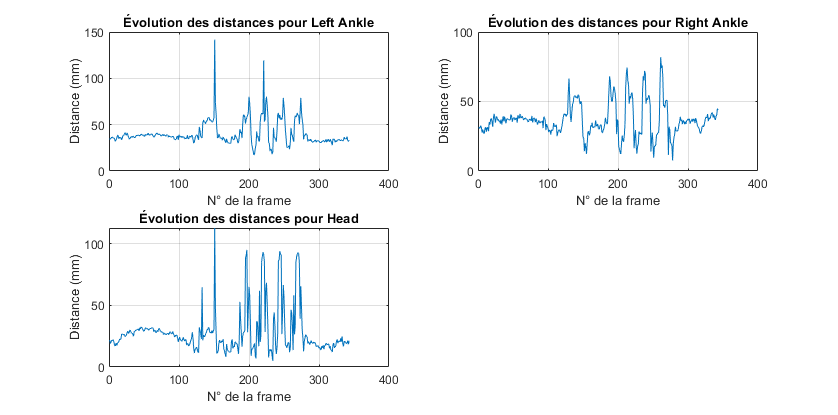
\includegraphics[width=\textwidth]{assets/Capture d'écran process/TX_ViconVSMocapIA/evolution_distance_Mocap2.png}
        \caption{Évolution de la distance}
    \end{figure}
    \begin{figure}[H]
        \centering
        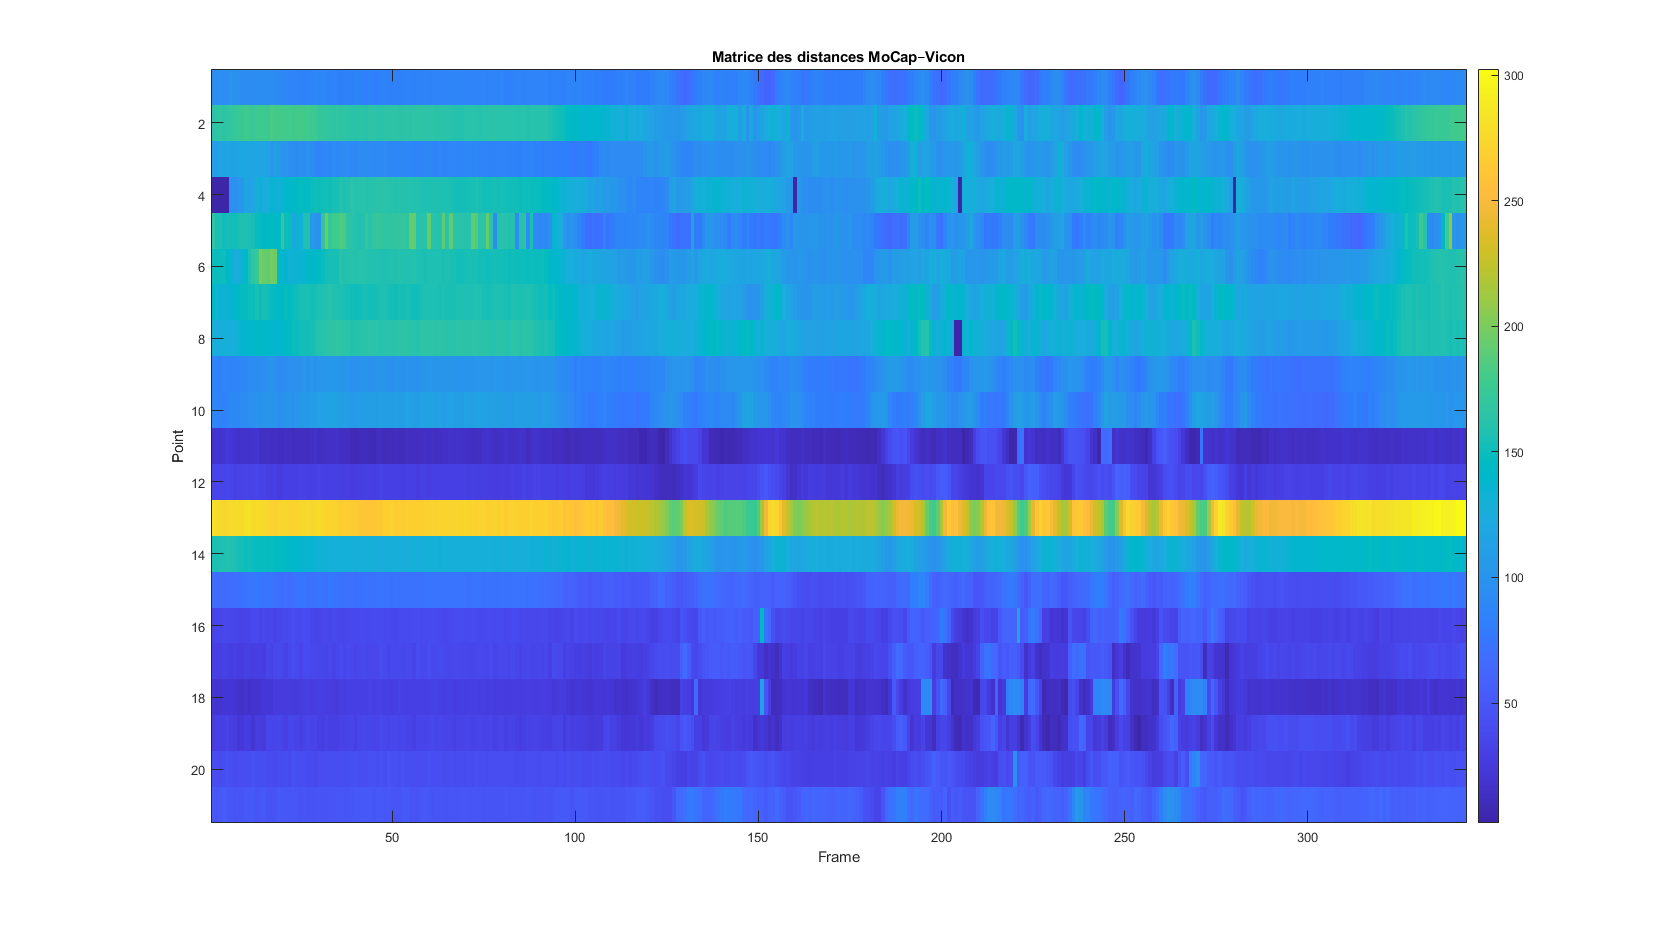
\includegraphics[width=\textwidth]{assets/Capture d'écran process/TX_ViconVSMocapIA/matrice_distances_result.png}
        \caption{Matrice des distances sur l'ensemble du mouvement entre chaque marqueur Vicon et MoCapIA}
    \end{figure}
    \begin{figure}[H]
        \centering
        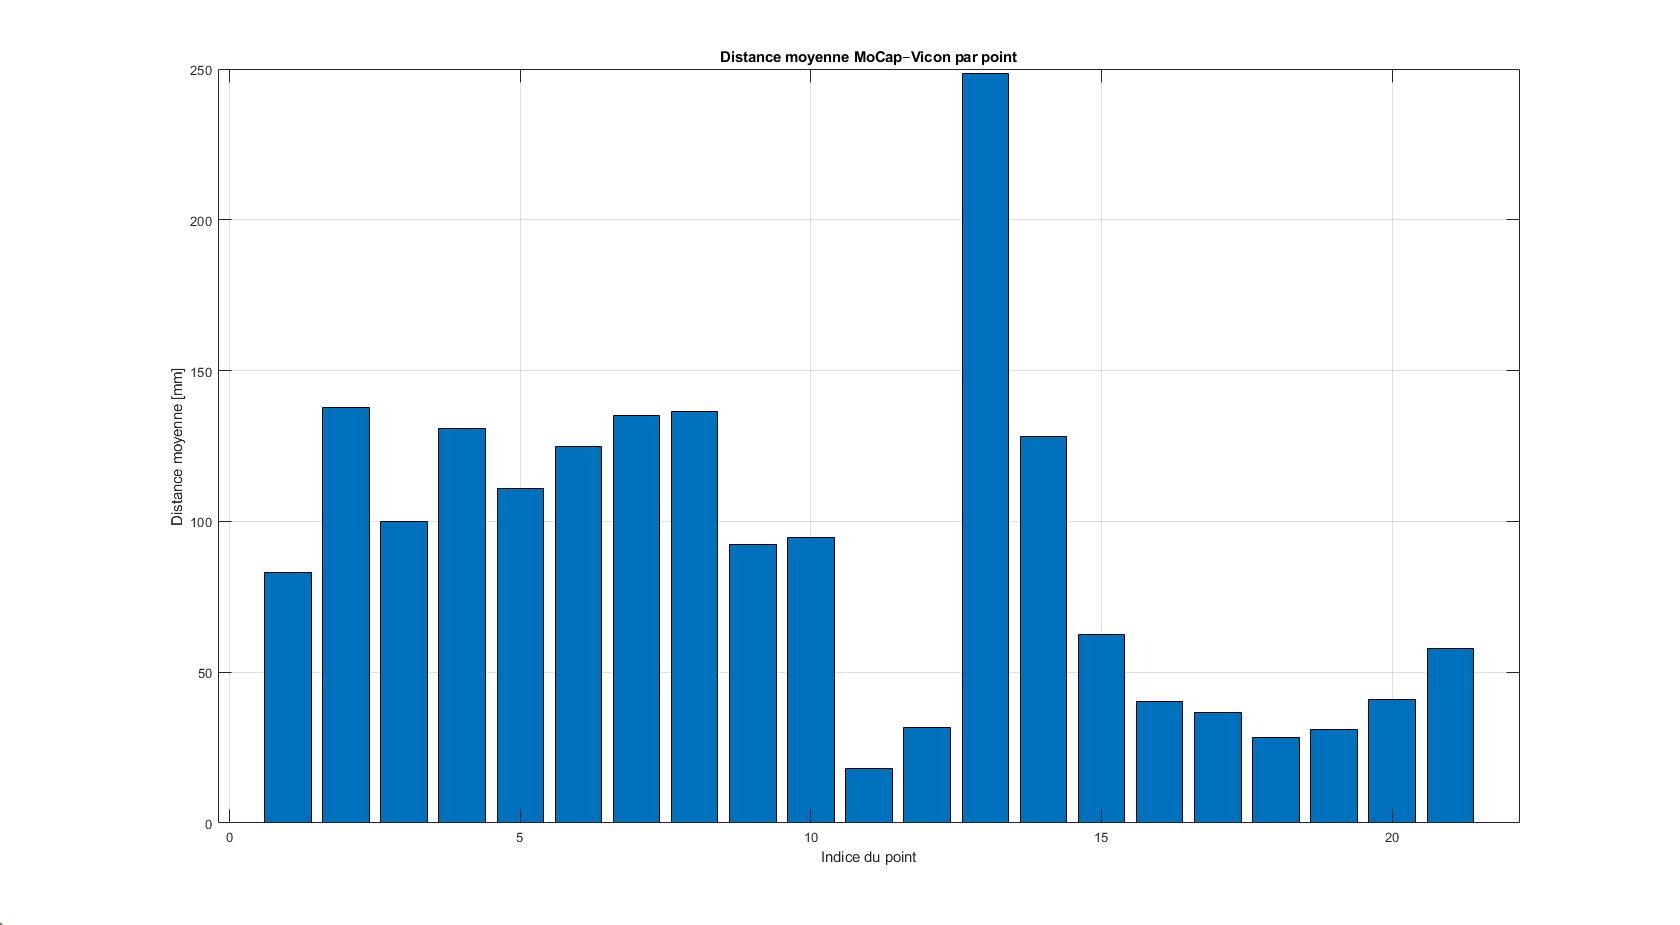
\includegraphics[width=\textwidth]{assets/Capture d'écran process/TX_ViconVSMocapIA/mean_distance.png}
        \caption{Distance moyenne entre chaque marqueur Vicon et MoCapIA}
    \end{figure}
    \begin{figure}[H]
        \centering
        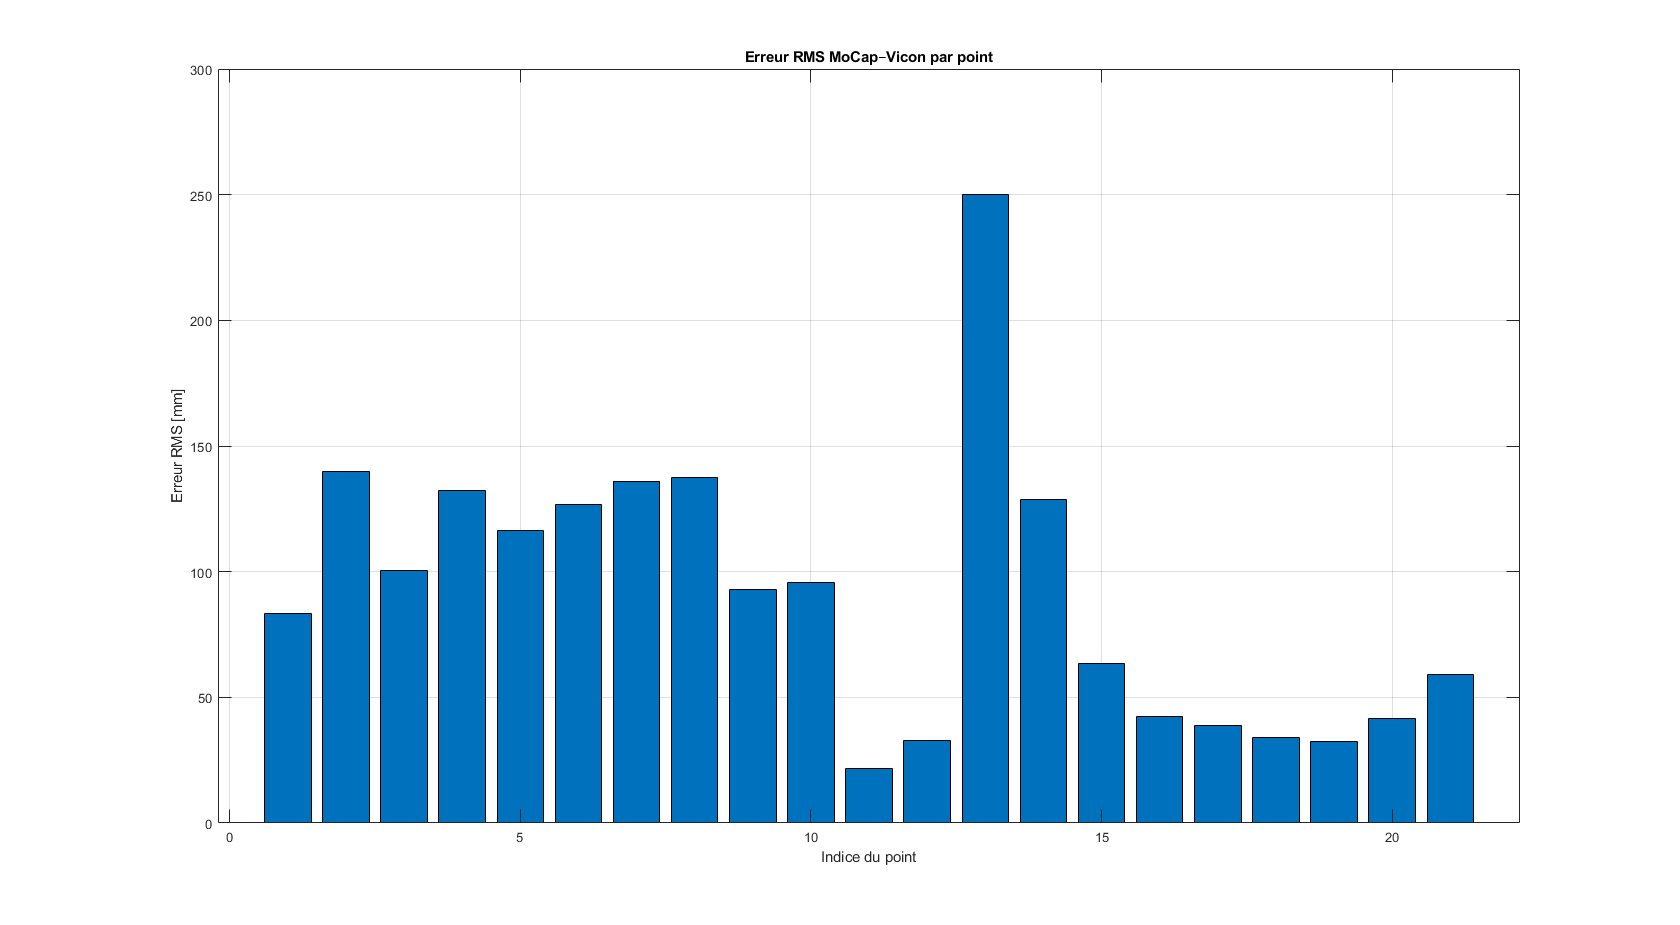
\includegraphics[width=\textwidth]{assets/Capture d'écran process/TX_ViconVSMocapIA/RMS_result.png}
        \caption{RMS des distances entre chaque marqueur Vicon et MoCapIA}
    \end{figure}

\section{Annexe 3 - résultat des autres filtres}
\label{Annexfiltres}

    Les filtres Kalman, LOESS, GCV Spline, Gaussien et Butterworth Speed ont également été testés sur les données 3D issues de MoCapIA. Les résultats, pas assez convaincant pour le filtrage d'un signal biomécanique, sont présentés dans les figures \ref{fig:kalman_result}, \ref{fig:loess_result}, \ref{fig:gcv_result}, \ref{fig:gaussian_result} et \ref{fig:butterworth_speed_result}.
    \begin{figure}[H]
        \centering
        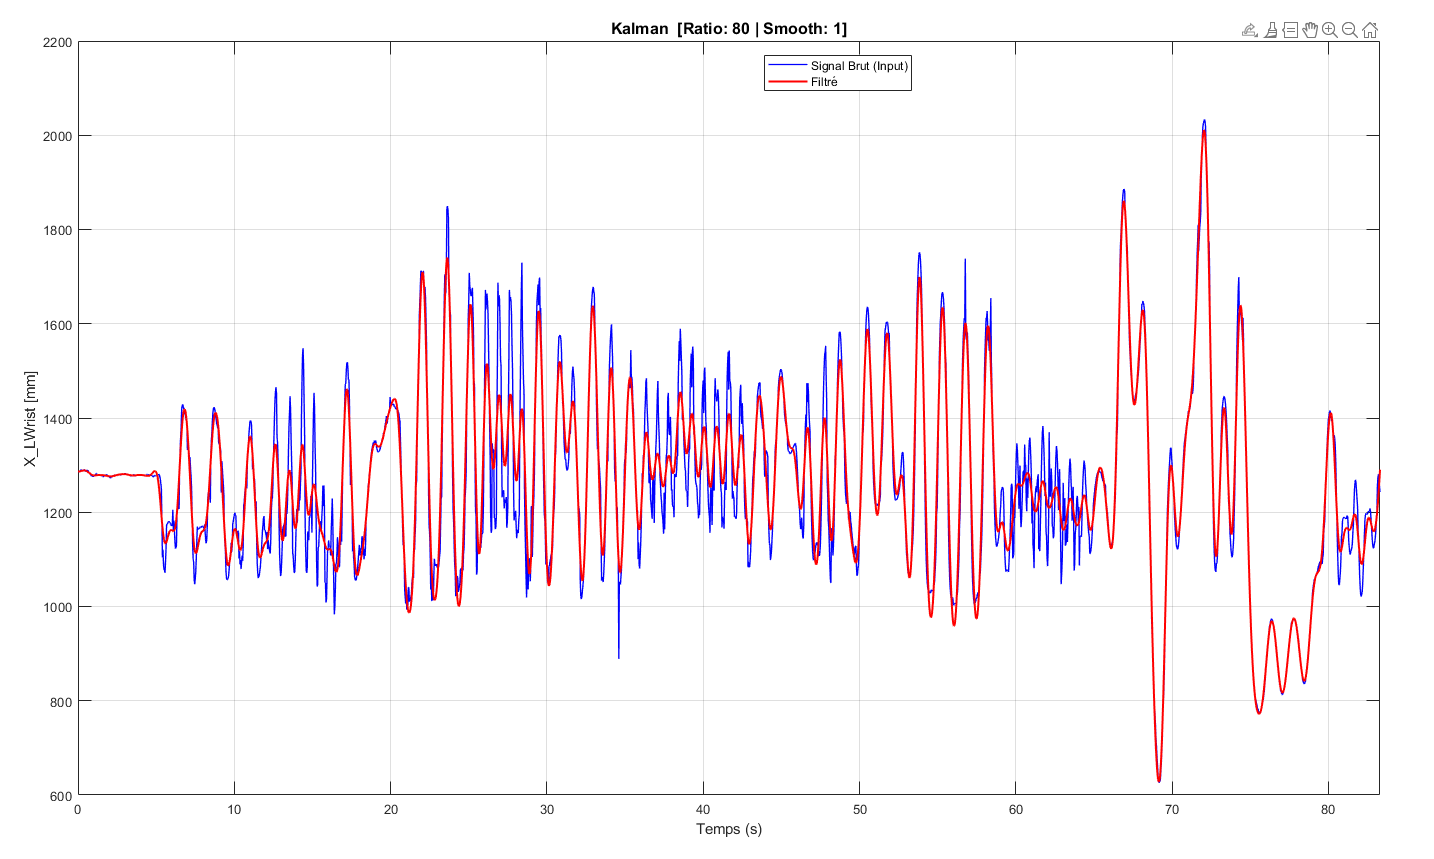
\includegraphics[width=\textwidth]{assets/Capture d'écran process/Tests Filtres 3D/valid/kalman.png}
        \caption{Résultat du filtre de Kalman avec un ratio de confiance de $150$}
        \label{fig:kalman_result}
    \end{figure}
    \begin{figure}[H]
        \centering
        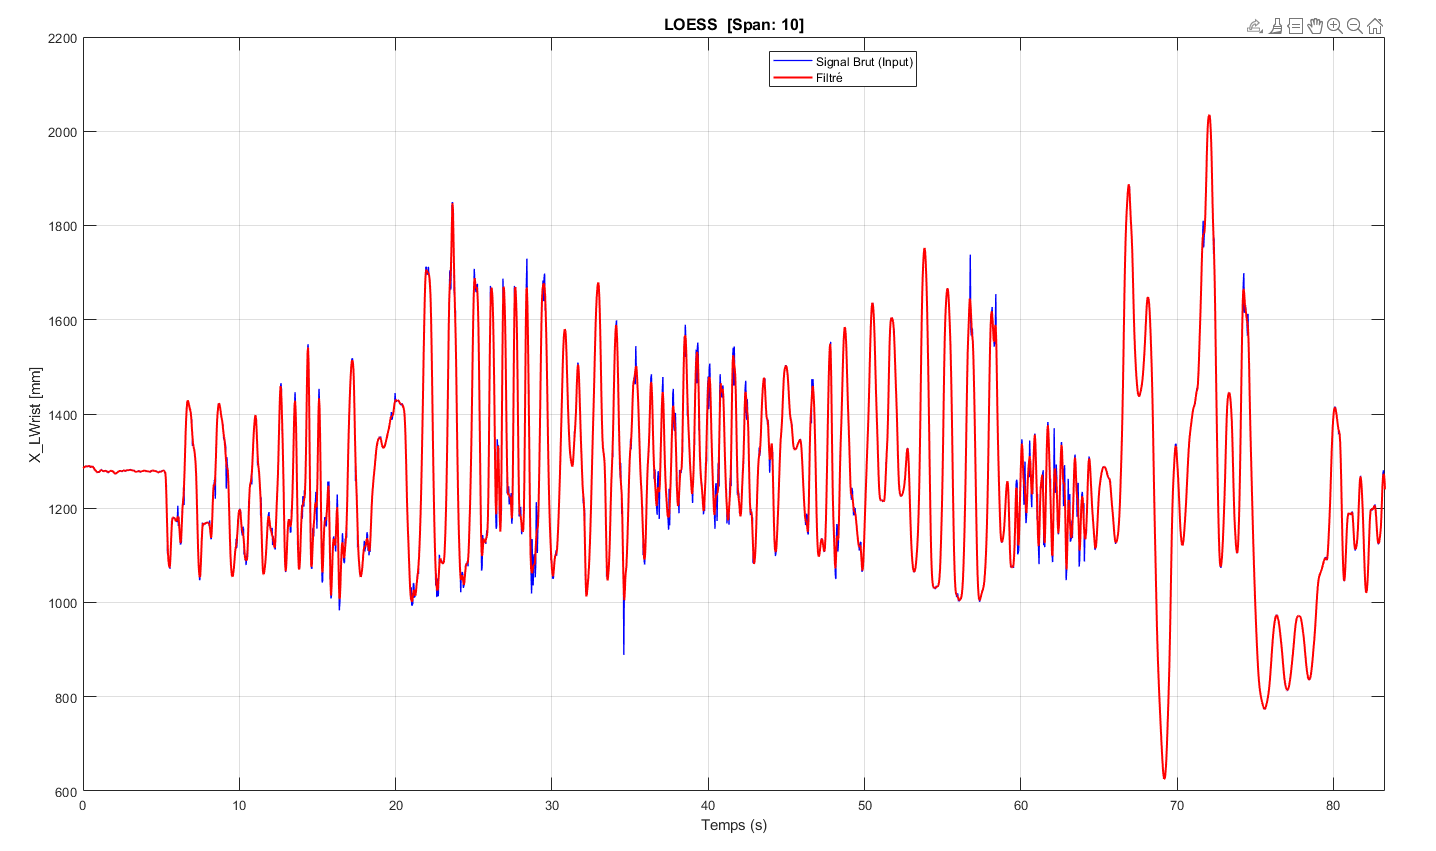
\includegraphics[width=\textwidth]{assets/Capture d'écran process/Tests Filtres 3D/valid/loess.png}
        \caption{Résultat du filtre LOESS avec un paramètre de lissage de $10$ valeurs}
        \label{fig:loess_result}
    \end{figure}
    \begin{figure}[H]
        \centering
        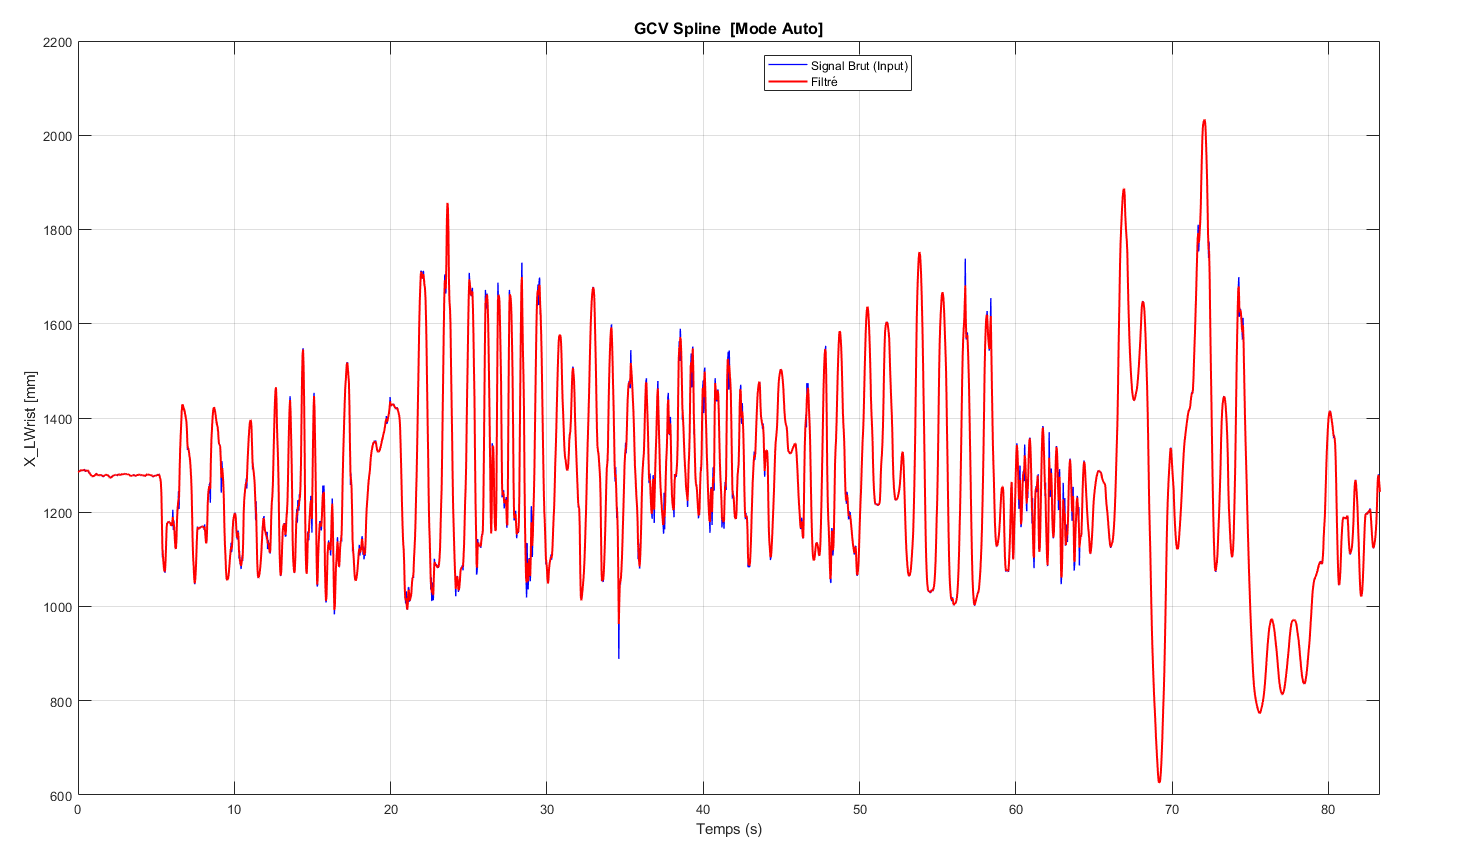
\includegraphics[width=\textwidth]{assets/Capture d'écran process/Tests Filtres 3D/valid/gcv_spline.png}
        \caption{Résultat du filtre GCV Spline}
        \label{fig:gcv_result}
    \end{figure}
    \begin{figure}[H]
        \centering
        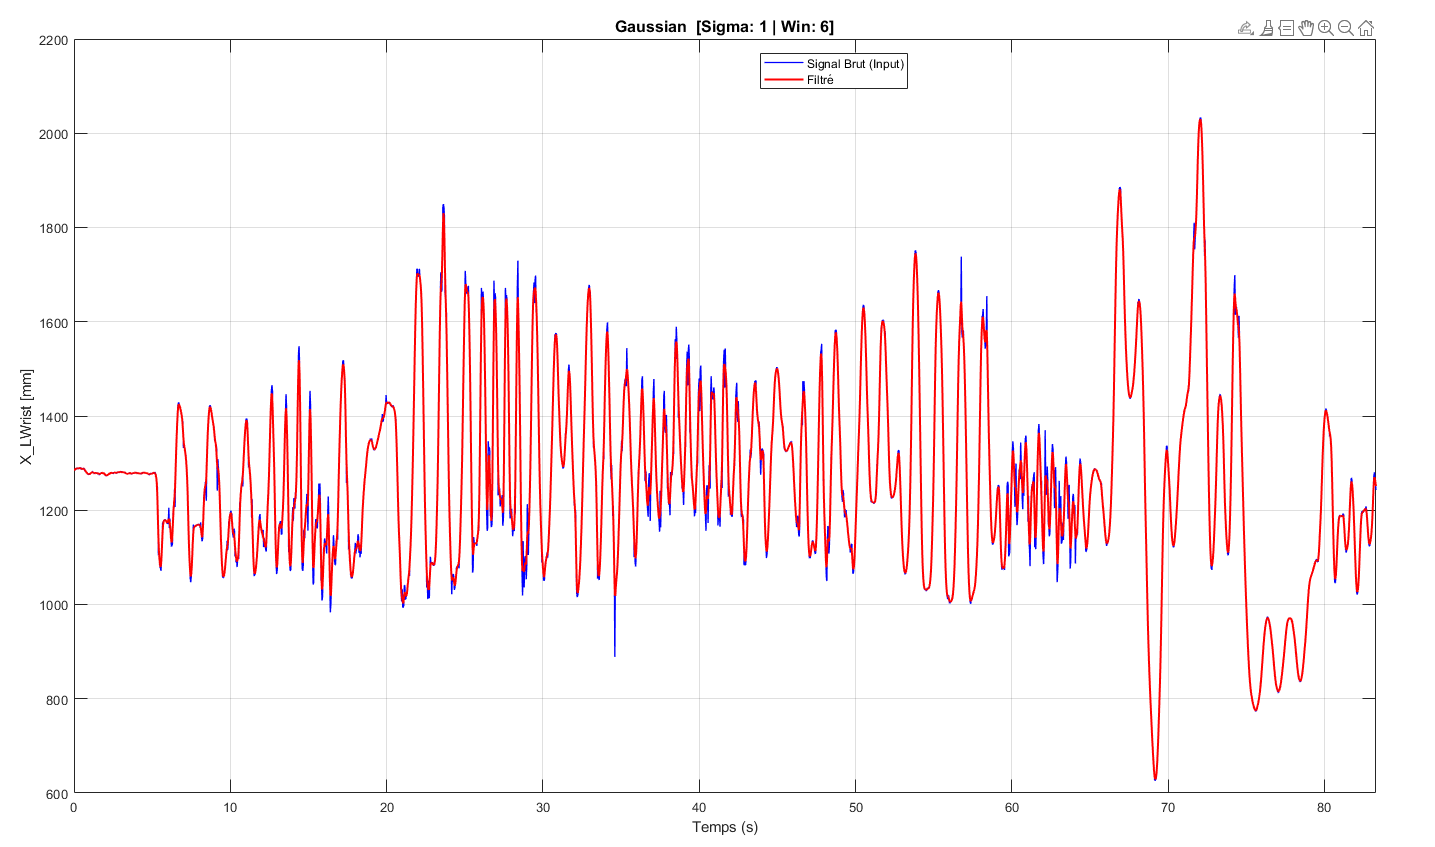
\includegraphics[width=\textwidth]{assets/Capture d'écran process/Tests Filtres 3D/valid/gaussian.png}
        \caption{Résultat du filtre Gaussien avec $sigma = 1$}
        \label{fig:gaussian_result}
    \end{figure}
    \begin{figure}[H]
        \centering
        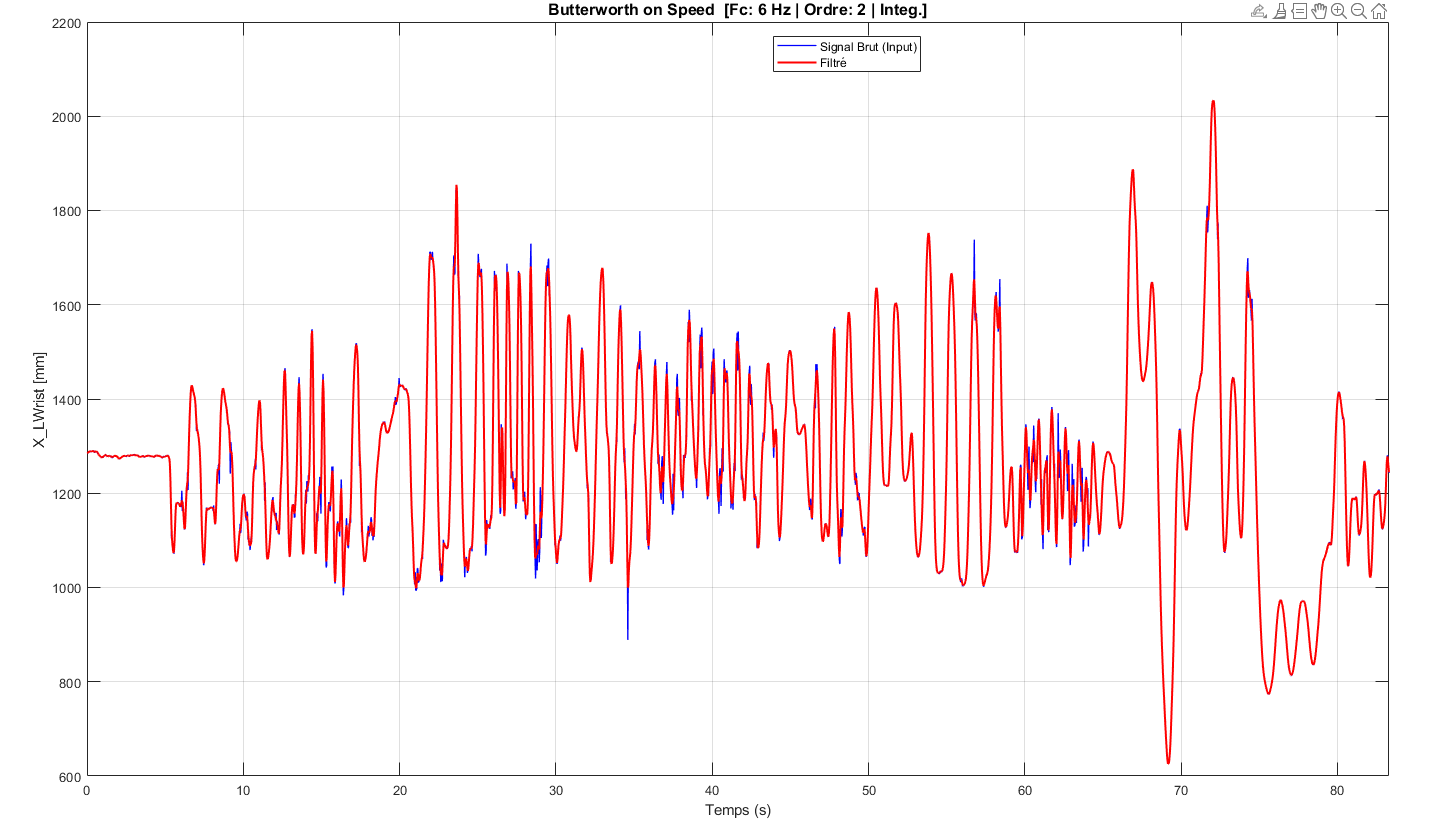
\includegraphics[width=\textwidth]{assets/Capture d'écran process/Tests Filtres 3D/valid/butterworth_speed.png}
        \caption{Résultat du filtre Butterworth Speed d'ordre 2 avec une fréquence de coupure de $6Hz$}
        \label{fig:butterworth_speed_result}
    \end{figure}

    \section{Annexe 4 - Analyse Bland-Altman de Vicon, SAM3D et MoCapIA}
    \label{AnnexBlandAltmanSAM3D}
        \begin{figure}[H]
            \centering
            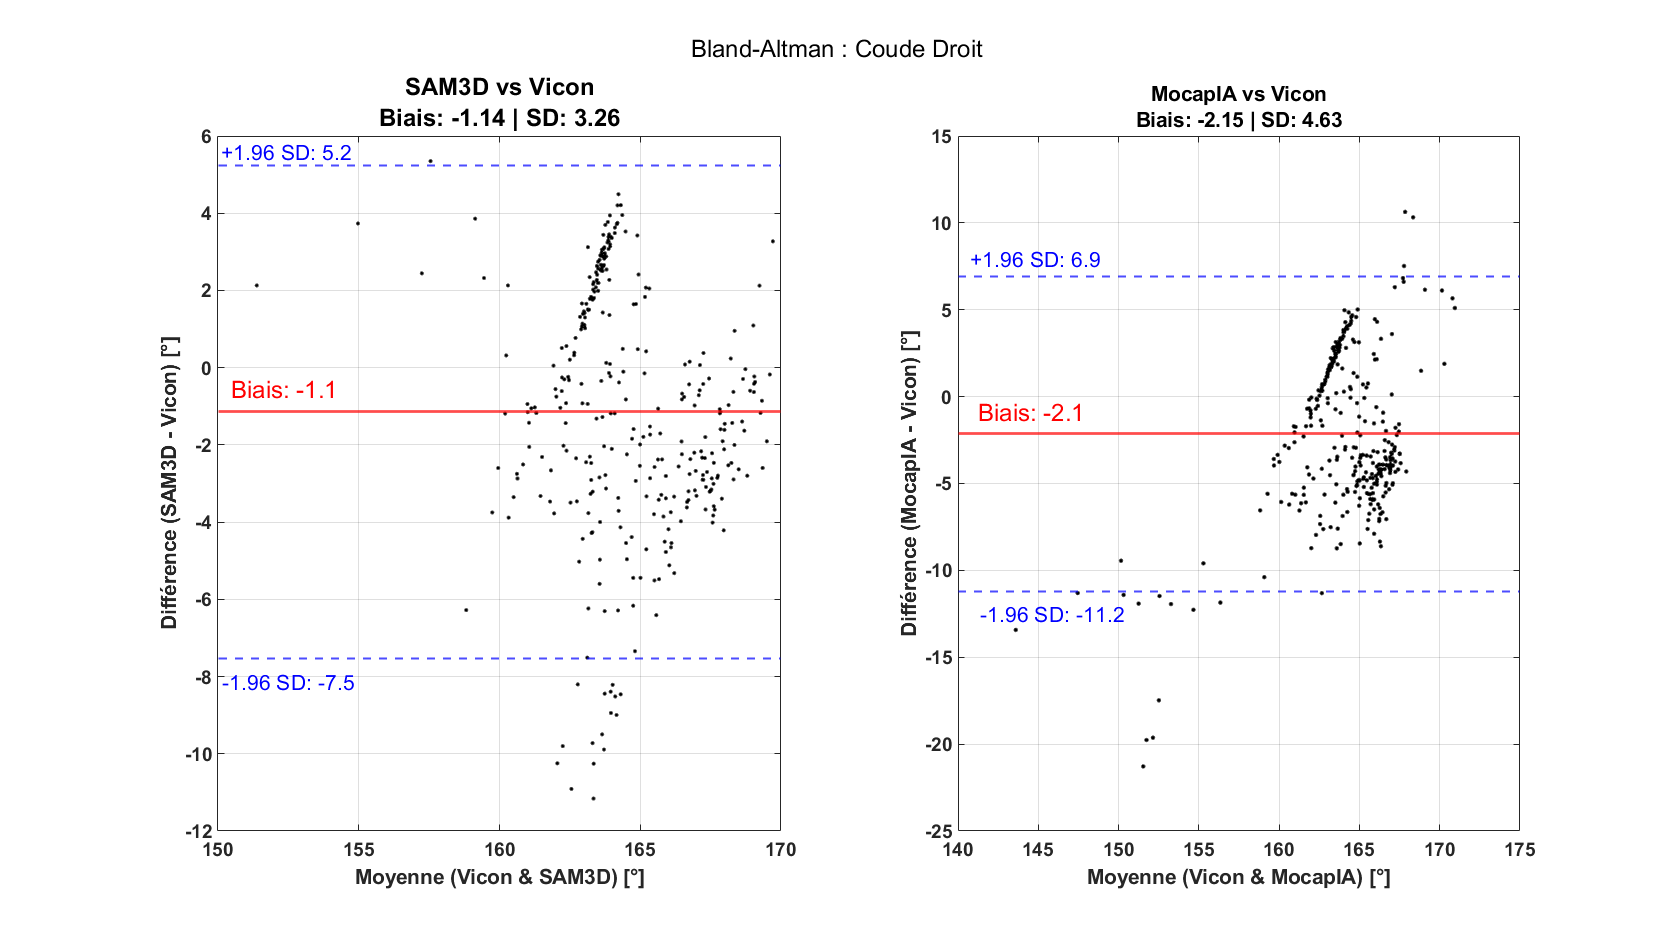
\includegraphics[width=\textwidth]{assets/Capture d'écran process/Vicon vs SAM3D vs MoCapIA/BlandAltman_Vicon_Mocap_sam3D_CoudeD.png}
            \caption{Analyse Bland-Altman entre Vicon, SAM 3D Body et MoCapIA pour le coude droit}
            \label{fig:bland_altman_vms1}
        \end{figure}
        \begin{figure}[H]
            \centering
            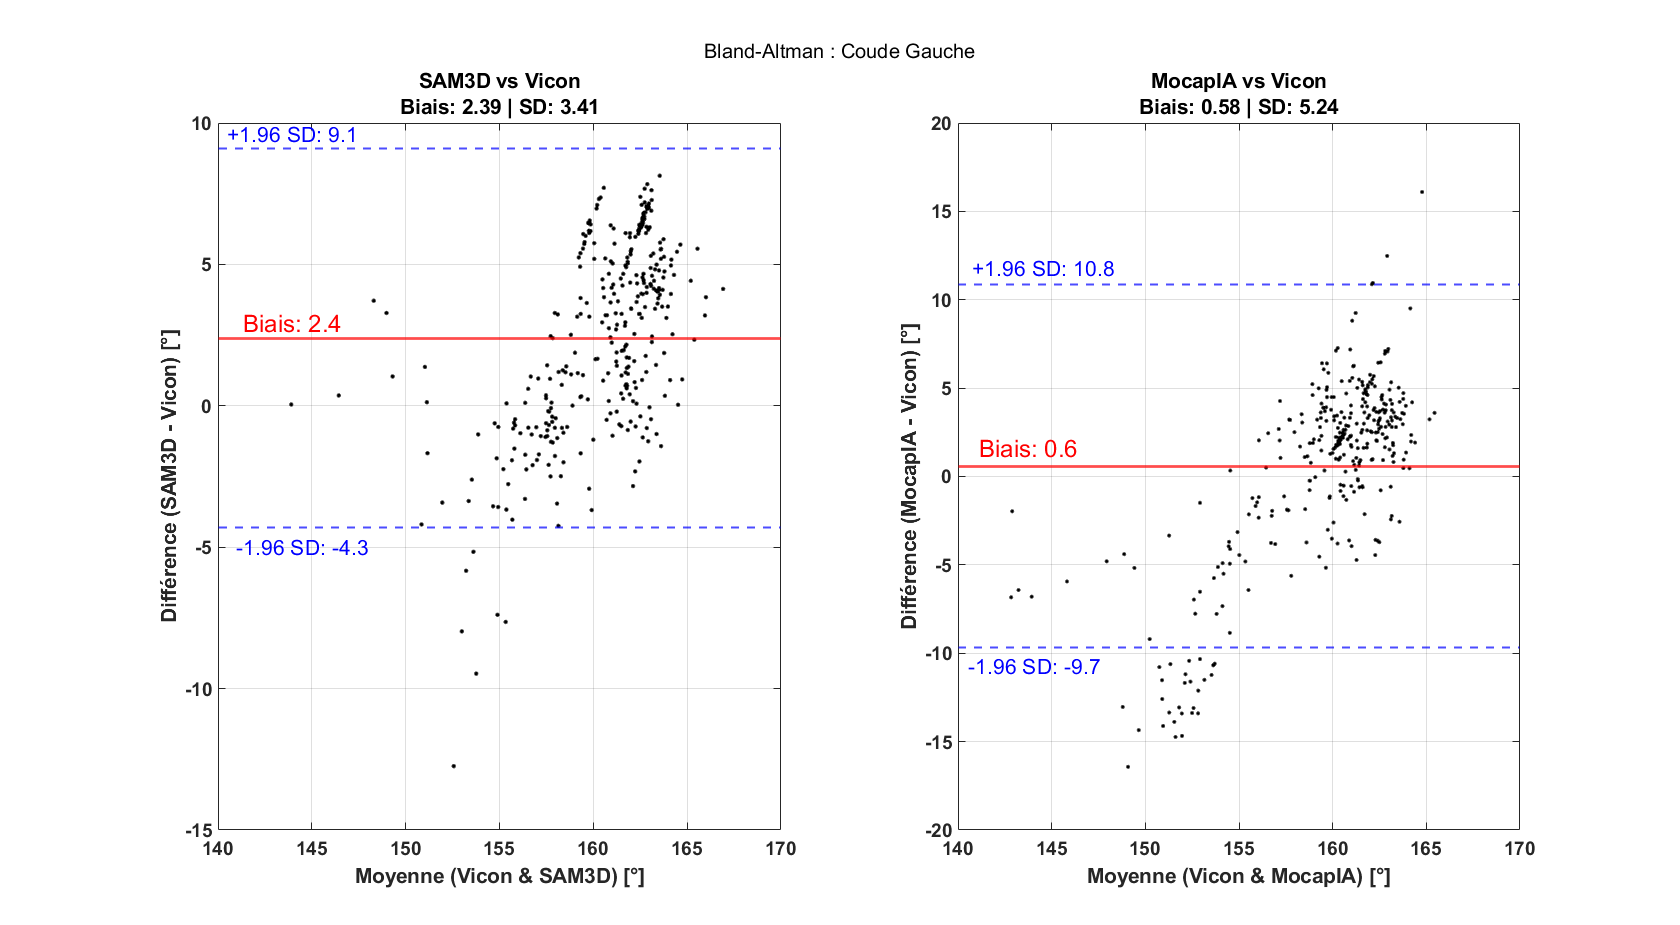
\includegraphics[width=\textwidth]{assets/Capture d'écran process/Vicon vs SAM3D vs MoCapIA/BlandAltman_Vicon_Mocap_sam3D_coudeG.png}
            \caption{Analyse Bland-Altman entre Vicon, SAM 3D Body et MoCapIA pour le coude gauche}
            \label{fig:bland_altman_vms2}
        \end{figure}
        \begin{figure}[H]
            \centering
            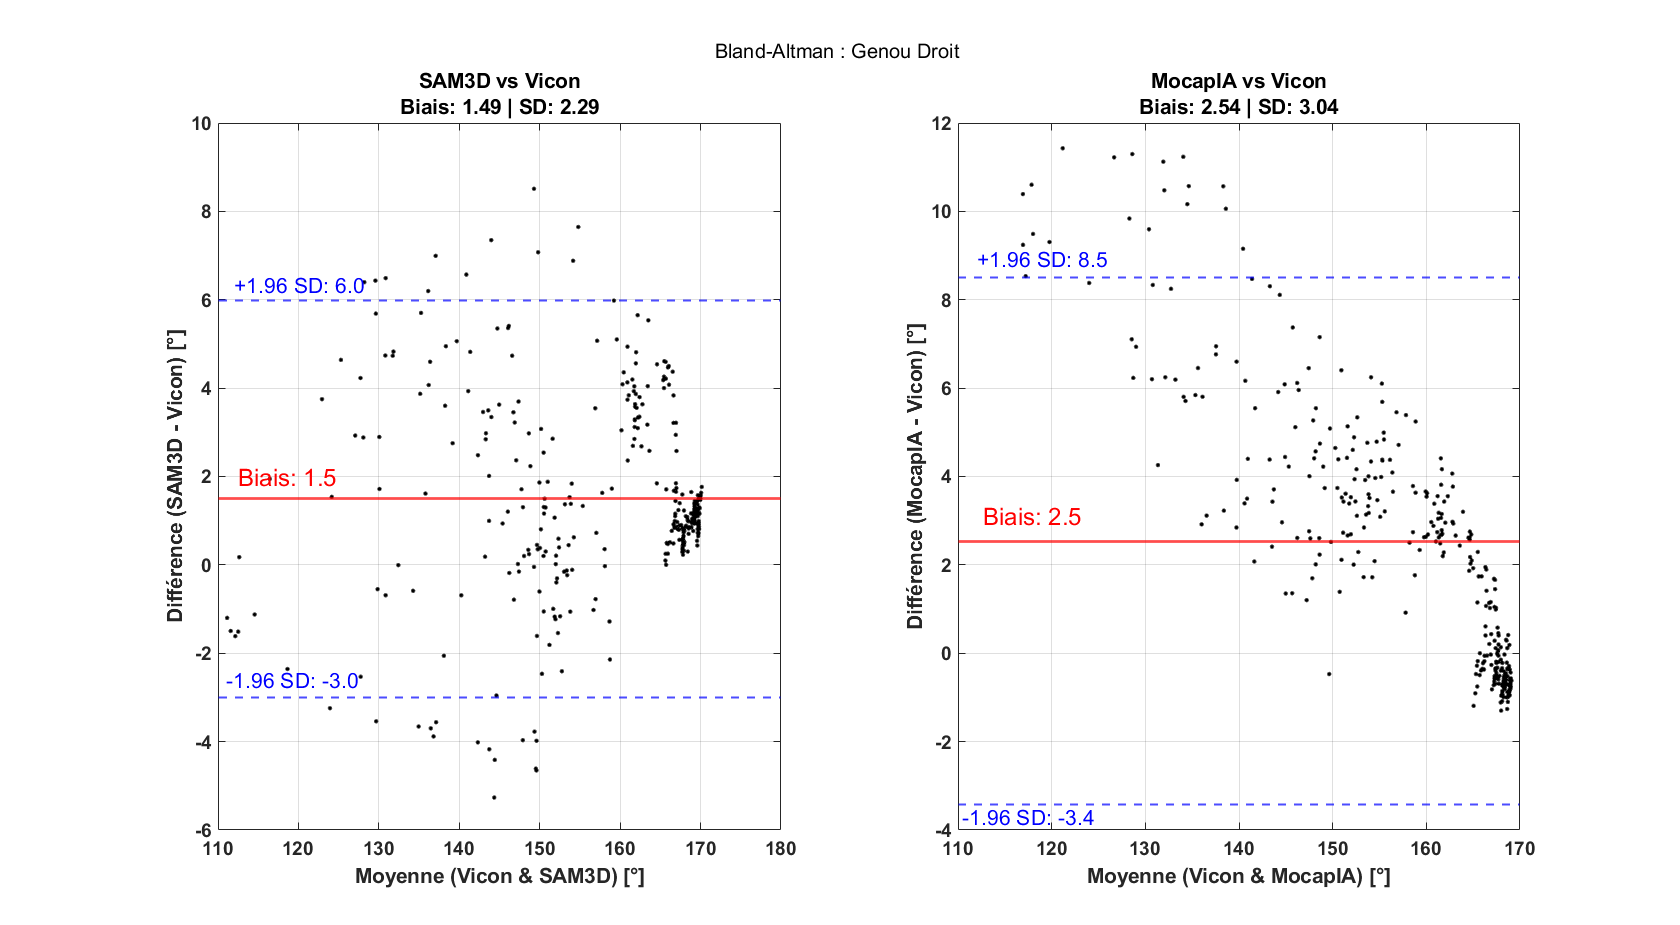
\includegraphics[width=\textwidth]{assets/Capture d'écran process/Vicon vs SAM3D vs MoCapIA/BlandAltman_Vicon_Mocap_sam3D_genouD.png}
            \caption{Analyse Bland-Altman entre Vicon, SAM 3D Body et MoCapIA pour le genou droit}
            \label{fig:bland_altman_vms3}
        \end{figure}
             
    
\end{document}
